%%%%%%%%%%%%%%%%%%%%%%%%%%%%%%%%%%%%%%%%%

% Lachaise Assignment
% LaTeX Template
% Version 1.0 (26/6/2018)
%
% This template originates from:
% http://www.LaTeXTemplates.com
%
% Authors:
% Marion Lachaise & François Févotte
% Vel (vel@LaTeXTemplates.com)
%
% License:
% CC BY-NC-SA 3.0 (http://creativecommons.org/licenses/by-nc-sa/3.0/)
% 
%%%%%%%%%%%%%%%%%%%%%%%%%%%%%%%%%%%%%%%%%

%----------------------------------------------------------------------------------------
%	PACKAGES AND OTHER DOCUMENT CONFIGURATIONS
%----------------------------------------------------------------------------------------

\documentclass[UTF8]{article}

%%%%%%%%%%%%%%%%%%%%%%%%%%%%%%%%%%%%%%%%%
% Lachaise Assignment
% Structure Specification File
% Version 1.0 (26/6/2018)
%
% This template originates from:
% http://www.LaTeXTemplates.com
%
% Authors:
% Marion Lachaise & François Févotte
% Vel (vel@LaTeXTemplates.com)
%
% License:
% CC BY-NC-SA 3.0 (http://creativecommons.org/licenses/by-nc-sa/3.0/)
% 
%%%%%%%%%%%%%%%%%%%%%%%%%%%%%%%%%%%%%%%%%

%----------------------------------------------------------------------------------------
%	PACKAGES AND OTHER DOCUMENT CONFIGURATIONS
%----------------------------------------------------------------------------------------

\usepackage{amsmath,amsfonts,stmaryrd,amssymb} % Math packages

\usepackage{enumerate} % Custom item numbers for enumerations

\usepackage[ruled]{algorithm2e} % Algorithms

\usepackage[framemethod=tikz]{mdframed} % Allows defining custom boxed/framed environments
\usepackage{cite}
\usepackage{url}
\usepackage{ctex}
\usepackage{graphicx}
\usepackage{subfigure}
\usepackage[utf8]{inputenc} % allow utf-8 input
\usepackage[T1]{fontenc}    % use 8-bit T1 fonts

\usepackage{listings} % File listings, with syntax highlighting
\lstset{
	basicstyle=\ttfamily, % Typeset listings in monospace font
}

%----------------------------------------------------------------------------------------
%	DOCUMENT MARGINS
%----------------------------------------------------------------------------------------

\usepackage{geometry} % Required for adjusting page dimensions and margins

\geometry{
	paper=a4paper, % Paper size, change to letterpaper for US letter size
	top=2.5cm, % Top margin
	bottom=3cm, % Bottom margin
	left=2.5cm, % Left margin
	right=2.5cm, % Right margin
	headheight=14pt, % Header height
	footskip=1.5cm, % Space from the bottom margin to the baseline of the footer
	headsep=1.2cm, % Space from the top margin to the baseline of the header
	%showframe, % Uncomment to show how the type block is set on the page
}

%----------------------------------------------------------------------------------------
%	FONTS
%----------------------------------------------------------------------------------------

\usepackage[utf8]{inputenc} % Required for inputting international characters
\usepackage[T1]{fontenc} % Output font encoding for international characters

\usepackage{XCharter} % Use the XCharter fonts

%----------------------------------------------------------------------------------------
%	COMMAND LINE ENVIRONMENT
%----------------------------------------------------------------------------------------

% Usage:
% \begin{commandline}
%	\begin{verbatim}
%		$ ls
%		
%		Applications	Desktop	...
%	\end{verbatim}
% \end{commandline}

\mdfdefinestyle{commandline}{
	leftmargin=10pt,
	rightmargin=10pt,
	innerleftmargin=15pt,
	middlelinecolor=black!50!white,
	middlelinewidth=2pt,
	frametitlerule=false,
	backgroundcolor=black!5!white,
	frametitle={Command Line},
	frametitlefont={\normalfont\sffamily\color{white}\hspace{-1em}},
	frametitlebackgroundcolor=black!50!white,
	nobreak,
}

% Define a custom environment for command-line snapshots
\newenvironment{commandline}{
	\medskip
	\begin{mdframed}[style=commandline]
}{
	\end{mdframed}
	\medskip
}

%----------------------------------------------------------------------------------------
%	FILE CONTENTS ENVIRONMENT
%----------------------------------------------------------------------------------------

% Usage:
% \begin{file}[optional filename, defaults to "File"]
%	File contents, for example, with a listings environment
% \end{file}

\mdfdefinestyle{file}{
	innertopmargin=1.6\baselineskip,
	innerbottommargin=0.8\baselineskip,
	topline=false, bottomline=false,
	leftline=false, rightline=false,
	leftmargin=2cm,
	rightmargin=2cm,
	singleextra={%
		\draw[fill=black!10!white](P)++(0,-1.2em)rectangle(P-|O);
		\node[anchor=north west]
		at(P-|O){\ttfamily\mdfilename};
		%
		\def\l{3em}
		\draw(O-|P)++(-\l,0)--++(\l,\l)--(P)--(P-|O)--(O)--cycle;
		\draw(O-|P)++(-\l,0)--++(0,\l)--++(\l,0);
	},
	nobreak,
}

% Define a custom environment for file contents
\newenvironment{file}[1][File]{ % Set the default filename to "File"
	\medskip
	\newcommand{\mdfilename}{#1}
	\begin{mdframed}[style=file]
}{
	\end{mdframed}
	\medskip
}

%----------------------------------------------------------------------------------------
%	NUMBERED QUESTIONS ENVIRONMENT
%----------------------------------------------------------------------------------------

% Usage:
% \begin{question}[optional title]
%	Question contents
% \end{question}

\mdfdefinestyle{question}{
	innertopmargin=1.2\baselineskip,
	innerbottommargin=0.8\baselineskip,
	roundcorner=5pt,
	nobreak,
	singleextra={%
		\draw(P-|O)node[xshift=1em,anchor=west,fill=white,draw,rounded corners=5pt]{%
		Question \theQuestion\questionTitle};
	},
}

\newcounter{Question} % Stores the current question number that gets iterated with each new question

% Define a custom environment for numbered questions
\newenvironment{question}[1][\unskip]{
	\bigskip
	\stepcounter{Question}
	\newcommand{\questionTitle}{~#1}
	\begin{mdframed}[style=question]
}{
	\end{mdframed}
	\medskip
}

%----------------------------------------------------------------------------------------
%	WARNING TEXT ENVIRONMENT
%----------------------------------------------------------------------------------------

% Usage:
% \begin{warn}[optional title, defaults to "Warning:"]
%	Contents
% \end{warn}

\mdfdefinestyle{warning}{
	topline=false, bottomline=false,
	leftline=false, rightline=false,
	nobreak,
	singleextra={%
		\draw(P-|O)++(-0.5em,0)node(tmp1){};
		\draw(P-|O)++(0.5em,0)node(tmp2){};
		\fill[black,rotate around={45:(P-|O)}](tmp1)rectangle(tmp2);
		\node at(P-|O){\color{white}\scriptsize\bf !};
		\draw[very thick](P-|O)++(0,-1em)--(O);%--(O-|P);
	}
}

% Define a custom environment for warning text
\newenvironment{warn}[1][Warning:]{ % Set the default warning to "Warning:"
	\medskip
	\begin{mdframed}[style=warning]
		\noindent{\textbf{#1}}
}{
	\end{mdframed}
}

%----------------------------------------------------------------------------------------
%	INFORMATION ENVIRONMENT
%----------------------------------------------------------------------------------------

% Usage:
% \begin{info}[optional title, defaults to "Info:"]
% 	contents
% 	\end{info}

\mdfdefinestyle{info}{%
	topline=false, bottomline=false,
	leftline=false, rightline=false,
	nobreak,
	singleextra={%
		\fill[black](P-|O)circle[radius=0.4em];
		\node at(P-|O){\color{white}\scriptsize\bf i};
		\draw[very thick](P-|O)++(0,-0.8em)--(O);%--(O-|P);
	}
}

% Define a custom environment for information
\newenvironment{info}[1][Info:]{ % Set the default title to "Info:"
	\medskip
	\begin{mdframed}[style=info]
		\noindent{\textbf{#1}}
}{
	\end{mdframed}
}
 % Include the file specifying the document structure and custom commands
\usepackage{multirow}
%----------------------------------------------------------------------------------------
%	ASSIGNMENT INFORMATION
%----------------------------------------------------------------------------------------

\title{2020年夏季Java小学期大作业\\ 实验报告} % Title of the assignment

\author{刘畅 \quad 2018011315 \\任一  \quad 2018011423 } % Author name and email address

\date{\today} % University, school and/or department name(s) and a date

%----------------------------------------------------------------------------------------
\lstset{
    % backgroundcolor=\color{red!50!green!50!blue!50},%代码块背景色为浅灰色
    rulesepcolor= \color{gray}, %代码块边框颜色
    breaklines=true,  %代码过长则换行
    numbers=left, %行号在左侧显示
    numberstyle= \small,%行号字体
    keywordstyle= \color{blue},%关键字颜色
    commentstyle=\color{gray}, %注释颜色
    frame=shadowbox%用方框框住代码块
}

\begin{document}

\maketitle % Print the title
\begin{center}
    \begin{tabular}{l  r}
    \hline
        \multicolumn{2}{c}{实验环境} \\ \hline
        minSdkVersion & 23 \\ \hline
        targetSdkVersion & 30 \\ \hline
        Android Studio Version&  4.0.1 \\ \hline
        % 集群GPU节点: & cn006-cn007\\ \hline
        % nvcc版本: & Cuda compilation tools, release 9.0, V9.0.176 \\ \hline% Date the experiment was performed

    \end{tabular}
\end{center}
\newpage
\section{代码结构}
本项目中,较为重要的文件夹有:java, assets, res。
\begin{itemize}
    \item {
        java文件夹下的com.java.renyi包为项目的java源码,它主要分为两个部分:
首先是db与LDA包,其中的代码实现了后端逻辑;其次根目录下是实现前端逻辑的所有代码。\newline
        
        db包中是数据库的相关代码,包括Repository, ViewModel, Database等各层级的代码,以及知疫学者和各国疫情数据的类。这部分的实现者为任一。

        LDA包中,是实现聚类算法的代码。这里的代码主要使用了开源仓库中的实现\url{https://github.com/jsksxs360/HanLDA}

        根目录下的前端代码主要分为两类:用于实现界面的activity和fragment,用于配置布局显示的adapter,viewbinder和viewfactory。
        该部分实现者为刘畅。
    }
    \item {
        assets文件夹下是聚类模型。即在本机上已经训练好的模型,在程序运行时需要加载。
    }
    \item {
        res文件夹下是前端实现的所有资源文件。
        其中,子文件夹drawable和mipmap存放图片文件,layout存放各界面的布局文件,
        values存放尺寸、颜色、字符串等文件,menu存放菜单栏有关文件,xml存放配置文件。
        该部分实现者为刘畅。
    }
\end{itemize}

\subsection*{具体分工}
刘畅:负责前端部分。包括前端页面跳转逻辑设计、前端各页面之间通信、各页面各控件的布局设计、后端数据的展示以及前端少量数据的存储。

任一:负责后端部分。设计数据库并实现数据库逻辑(上下拉和搜索逻辑、离线数据存储)、解析API数据、实现并调优聚类功能、申请微信SDK。


\clearpage
\section{具体实现}
\subsection{前端部分}
\subsubsection{总体逻辑}
前端总体跳转逻辑如下:点击app后直接进入主页面,主页面通过顶部工具栏实现搜索功能,
工具栏下方为标签栏,通过滑动或点击实现标签页切换,点击标签栏最右方按钮跳转至标签编辑页面。

点击工具栏左侧的抽屉按钮,可以打开应用抽屉,其中放置了多个选项,包括疫情数据、疫情图谱、知疫学者和夜间模式。
点击可跳转至相应的activity或执行相应的功能。
\subsubsection{新闻分类与新闻列表}
市面上的新闻资讯app主要采用滑动标签页的效果展示分类和对应分类下的新闻列表。
实现这种效果的方法很多,我采用的方法是,用tablayout实现顶部标签页,viewpager实现滑动效果,并通过viewpager绑定
新闻列表展示的fragment。fragment中就是对应类别的新闻列表了,采用smartfreshlayout嵌套recyclerview能够轻松实现
表项内容的定制以及上拉更多与下拉刷新的功能。通过对每一项添加点击事件监听,可以进入对应的新闻详情页,它们之间通过intent通信。

此页面的点击变灰功能配合后端进行实现,在用户点击进入详情页并返回后,前端会执行操作更改数据库对应数据项的viewed字段。
而在新闻列表recyclerview的数据绑定中则根据该字段的值设置文字颜色。

\begin{figure}[htbp]
    \centering
    \subfigure[news列表]{
    \begin{minipage}[t]{0.5\linewidth}
    \centering
    
\includegraphics[width=0.5\textwidth]{newslist1.jpg}
    %\caption{fig1}
    \end{minipage}%
    }%
    \subfigure[paper列表]{
    \begin{minipage}[t]{0.5\linewidth}
    \centering
    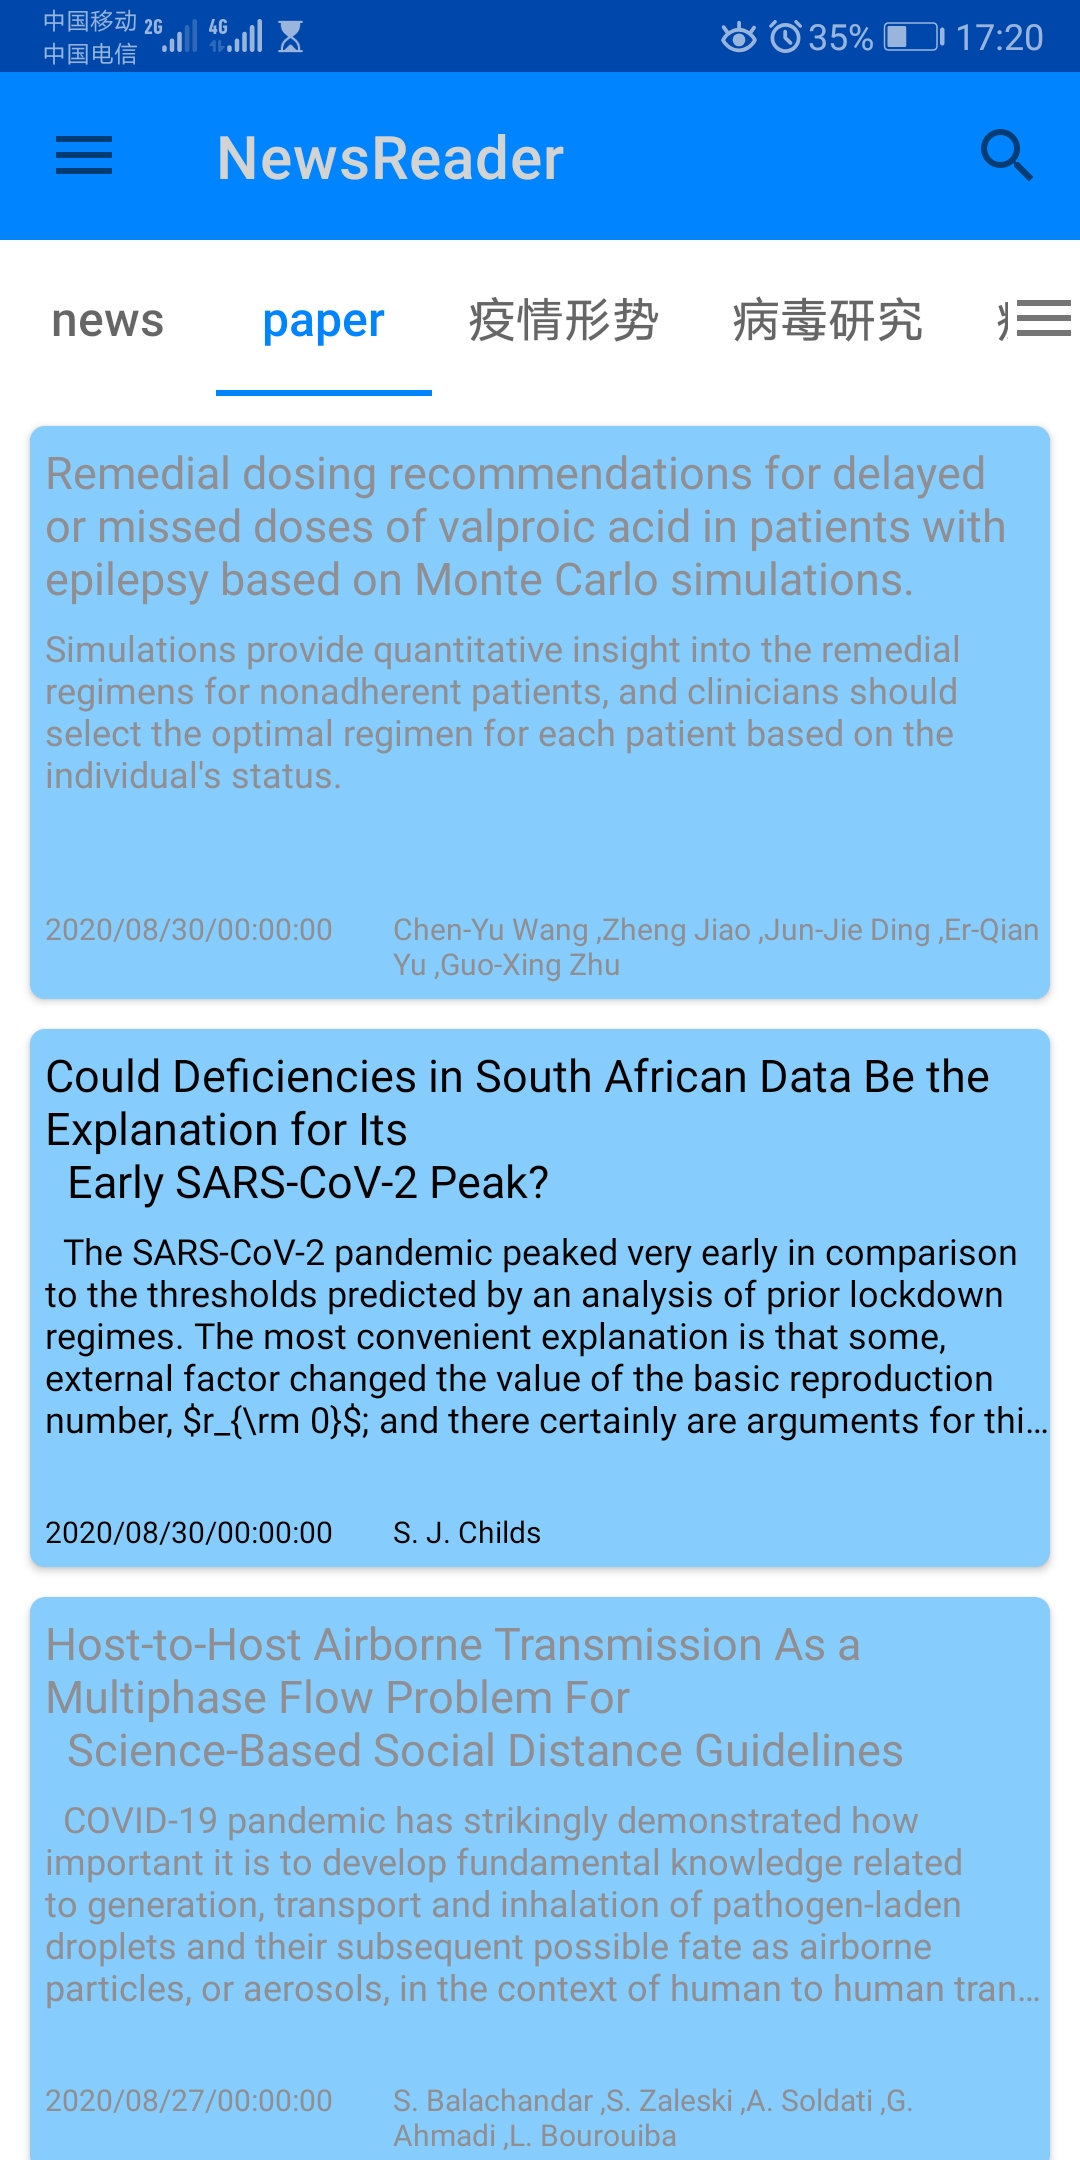
\includegraphics[width=0.5\textwidth]{newslist2.jpg}
    %\caption{fig2}
    \end{minipage}%
    }%
    \centering
    \caption{新闻分类与新闻列表}
    \end{figure}


\textbf{\heiti 难点:}
在实现的过程中这部分出现过3个问题。

\begin{itemize}
    \item {
        标签编辑后标签与fragment的内容不对应。比如首次进入应用时第一个标签是"news",
        第二个标签为"paper",删除第一个标签后,显示第一个标签为"paper",但对应fragment中为"news"的内容。
        通过重写fragment的onResume方法,发现当前标签为本应为"paper"的fragment输出的当前tag值竟然是"news"。
        
        这个问题与framgent生命周期管理有关。默认情况下,FragmentPagerAdapter没有在onDestroy方法中添加销毁fragment实例的逻辑,因此自定义的HomePagerAdapter
        应该继承FragmentStatePagerAdapter。
    }
    \item {
        当标签多于3个时,标签页来回切换会出现"IllegalStateException: Bindings already cleared"错误,
        这是由于viewpager有回收fragment的机制,如果被回收,再次回到该标签页会导致视图bind失败。
        最简单的解决办法是给viewpager添加缓存机制,这里我根据需要把缓存的fragment数设置为了7。
    }

    \item {
        测试时发现点击变灰没有问题,但是某些项也会出现“未点击变灰”。调试输出后发现后端数据正常,但是前段这个玄学问题依然存在。
        困惑之际队友发现我的NewsListAdapter代码中少了对默认未点击情况的处理,增加之后便一切正常。看来在java代码与xml混用的时候还是要小心。
    }
\end{itemize}

\subsubsection{标签编辑}
标签编辑页要实现拖拽等动态效果,我找到了一个第三方Layout,类名为:DragGridLayout。
该类已经封装好了拖拽、删除等常用功能,根据本处需求对代码和资源文件加以修改即可。

\textbf{\heiti 难点:}
值得一提的是如何获得用户的修改结果并返回给主页面呢?第三方Layout本身并没有提供这样的功能。
这里我采用了一种原始的方式,通过根节点rootView递归遍历所有的子view/viewGroup,并提取出父节点为GridLayout的TextView中的文字。
为了让用户退出程序后依然能够看到标签修改后的结果,每次修改完成返回主页面时都将标签列表保存到了SharedPreferences中,创建页面时则从中读取标签列表。

\begin{figure}[htbp]
    \centering
    \subfigure[标签编辑页]{
    \begin{minipage}[t]{0.5\linewidth}
    \centering
    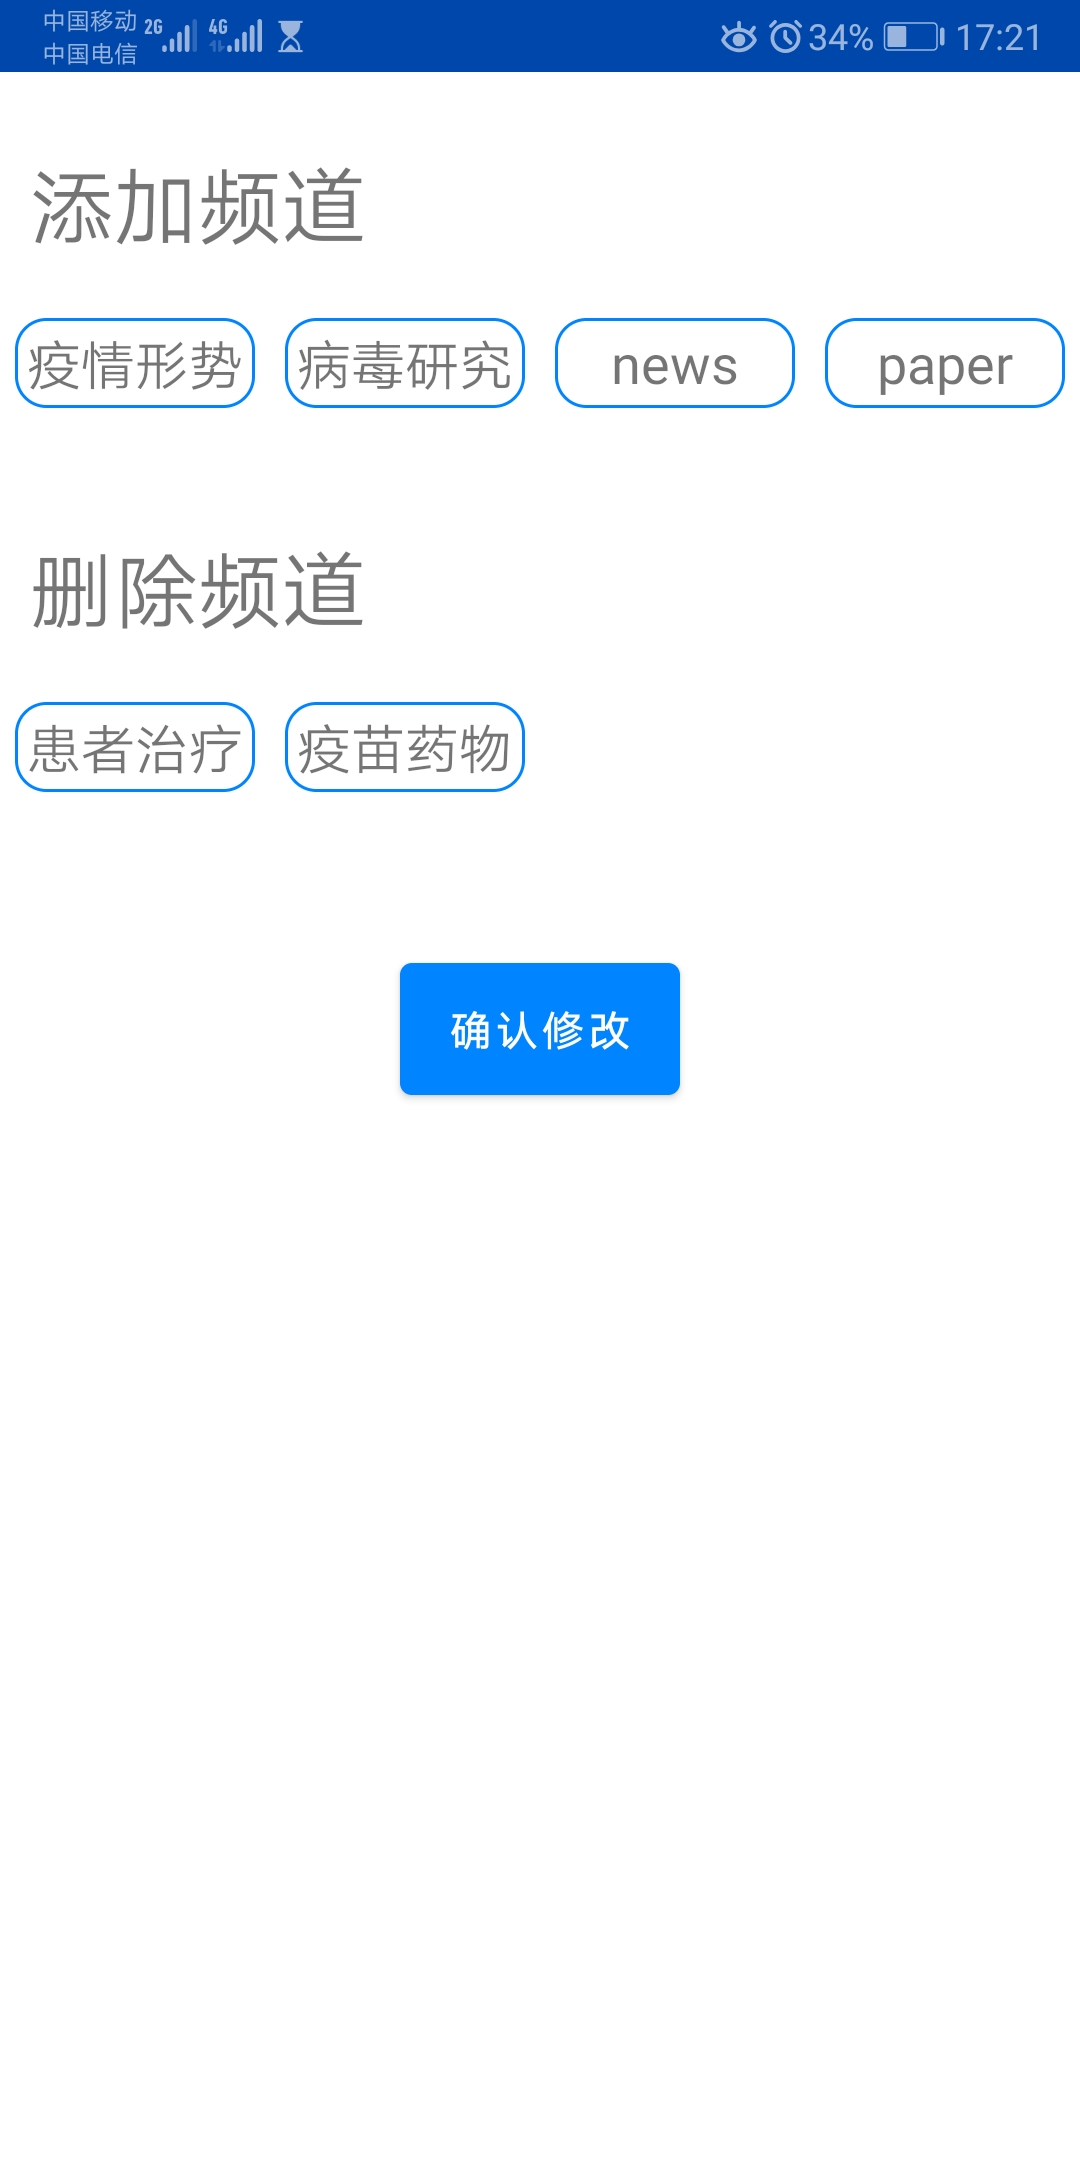
\includegraphics[width=0.5\textwidth]{tagedit1}
    %\caption{fig1}
    \end{minipage}%
    }%
    \subfigure[编辑后效果]{
    \begin{minipage}[t]{0.5\linewidth}
    \centering
    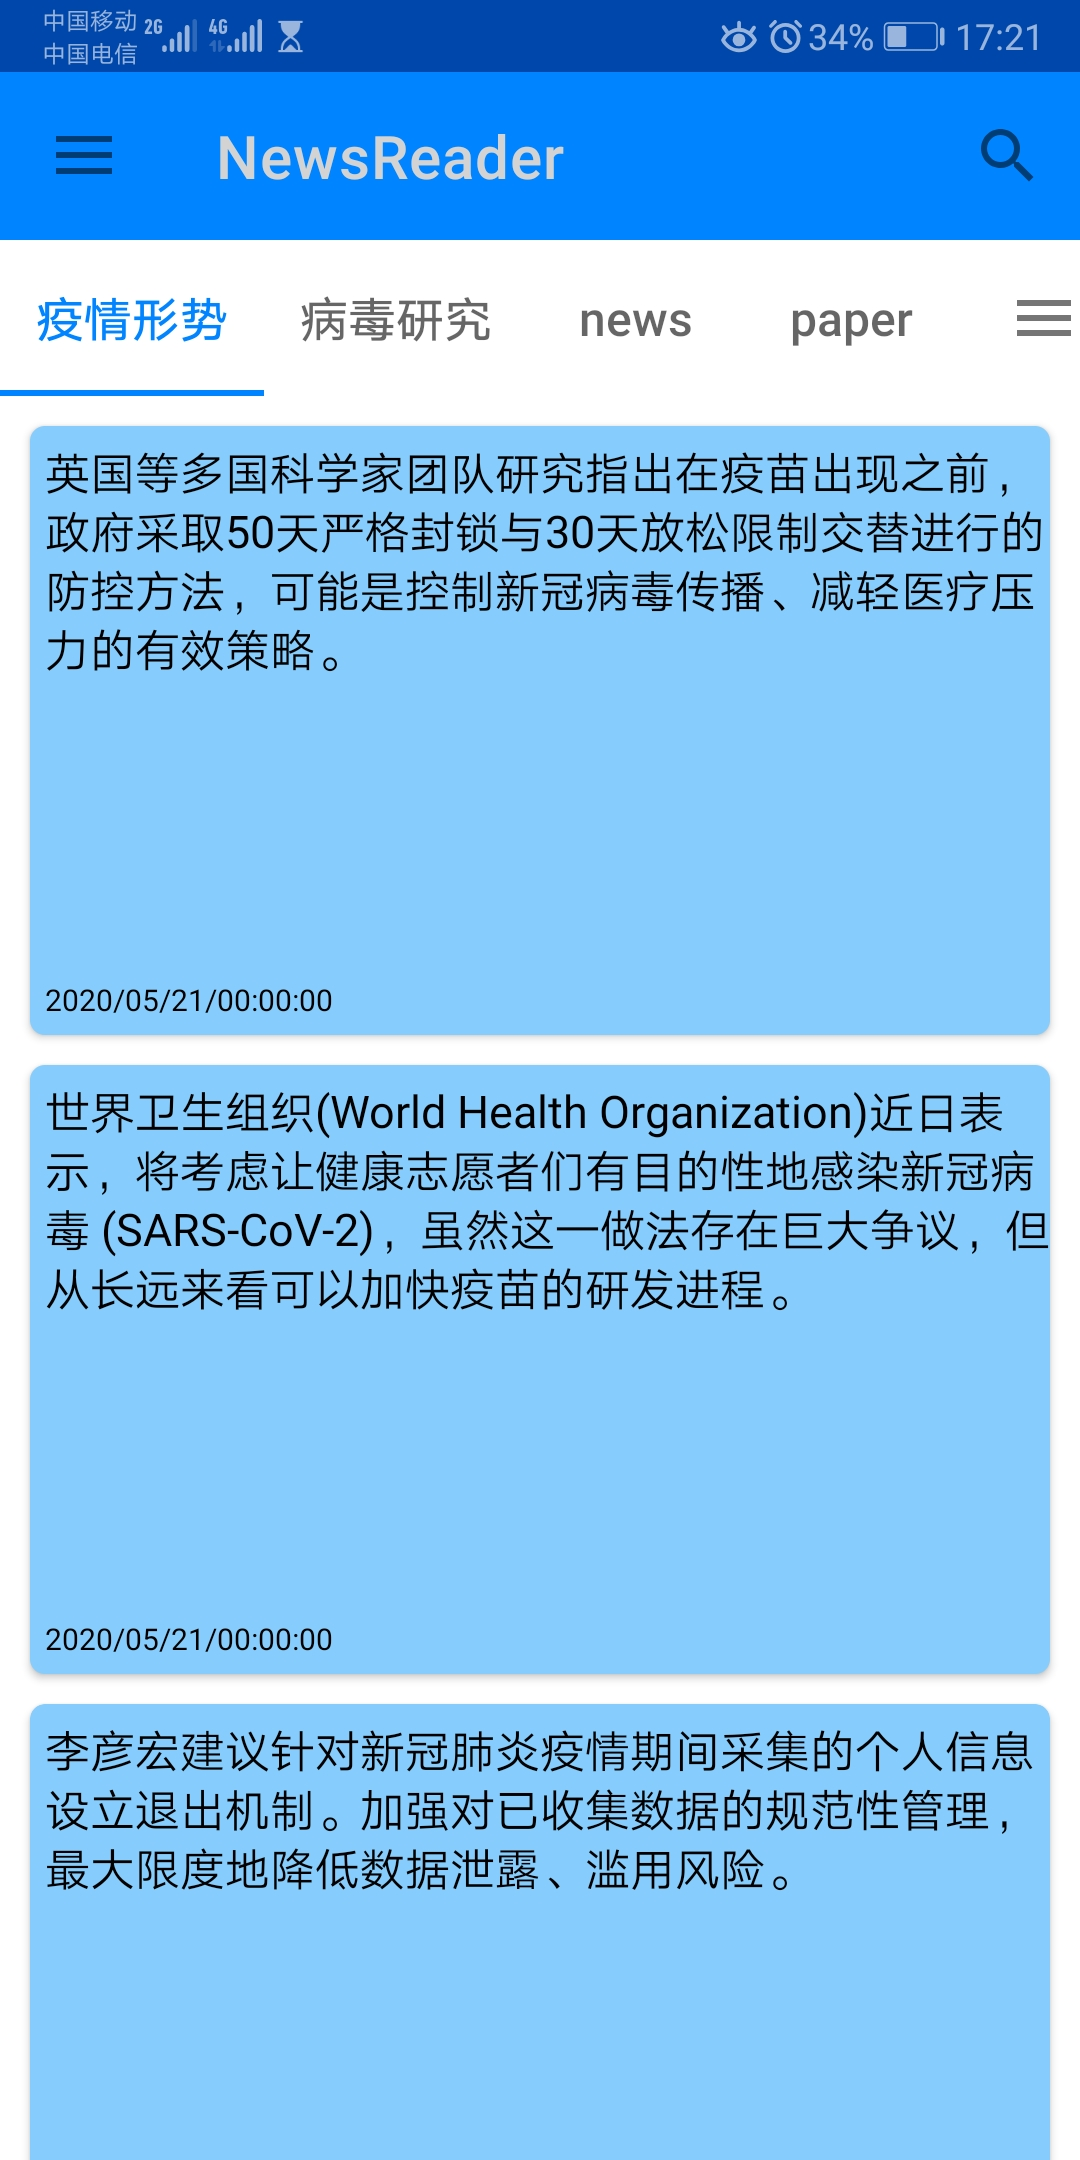
\includegraphics[width=0.5\textwidth]{tagedit2}
    %\caption{fig2}
    \end{minipage}%
    }%
    \centering
    \caption{标签编辑界面与编辑成功效果}
    \end{figure}


\subsubsection{新闻搜索与历史记录}
谷歌官方的SearchView控件对这些功能有强大的支持。通过在应用清单中进行配置,可以隐式地向搜索展示页面传递搜索字符串query。
搜索展示页面的逻辑与新闻列表页十分类似。而历史记录则继承了官方提供的SearchRecentSuggestionsProvider,可以方便地将近期浏览记录保存到本地。


    % \begin{figure}[h]
    %     \label{Ratio}
    %     \centering
    %         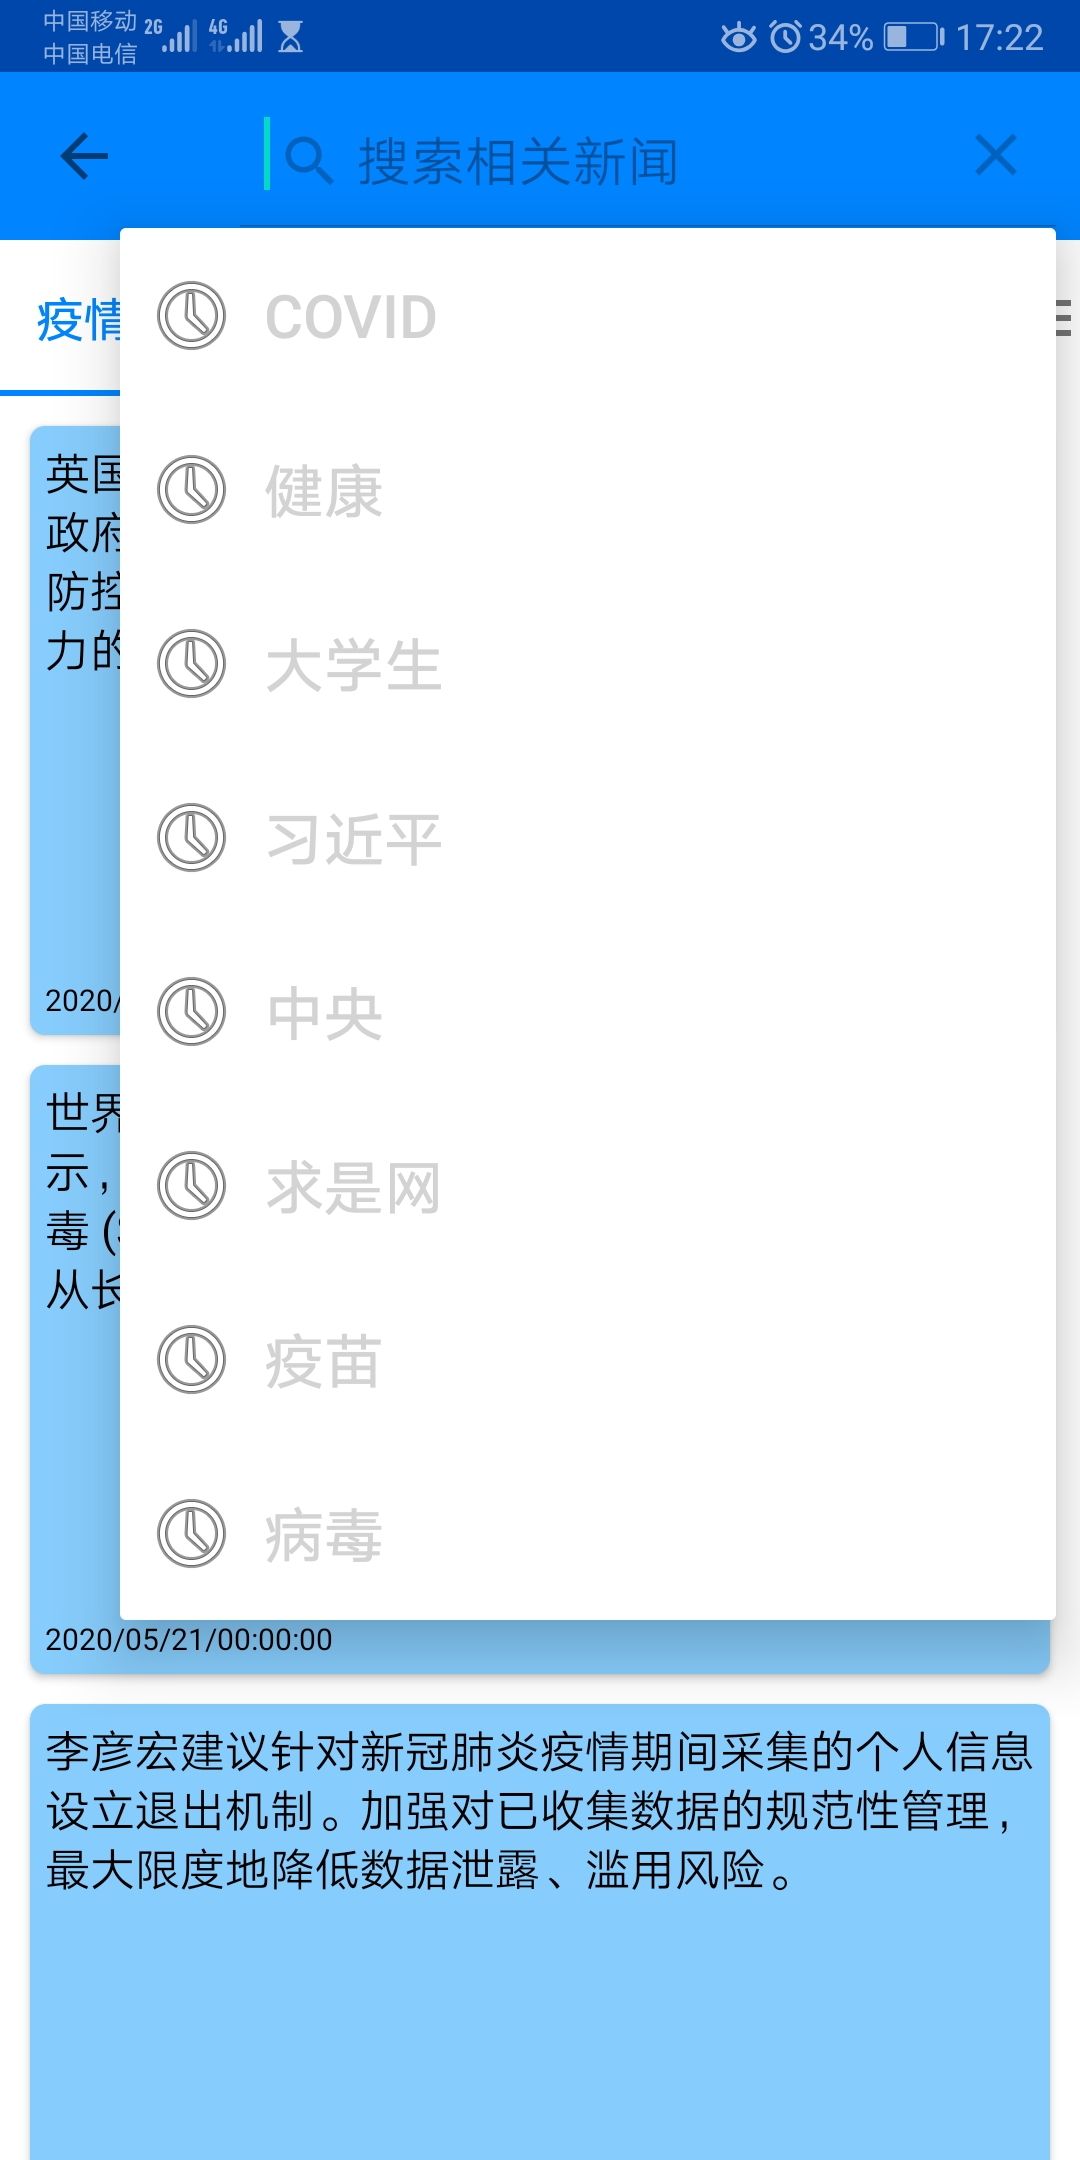
\includegraphics[height=0.5\textwidth]{search1}
    %         \caption{搜索页面和历史搜索记录}
    %     \end{figure}

\begin{figure}[htbp]
    \centering
    \subfigure[搜索页面和历史搜索记录]{
        \begin{minipage}[t]{0.3\linewidth}
        \centering
        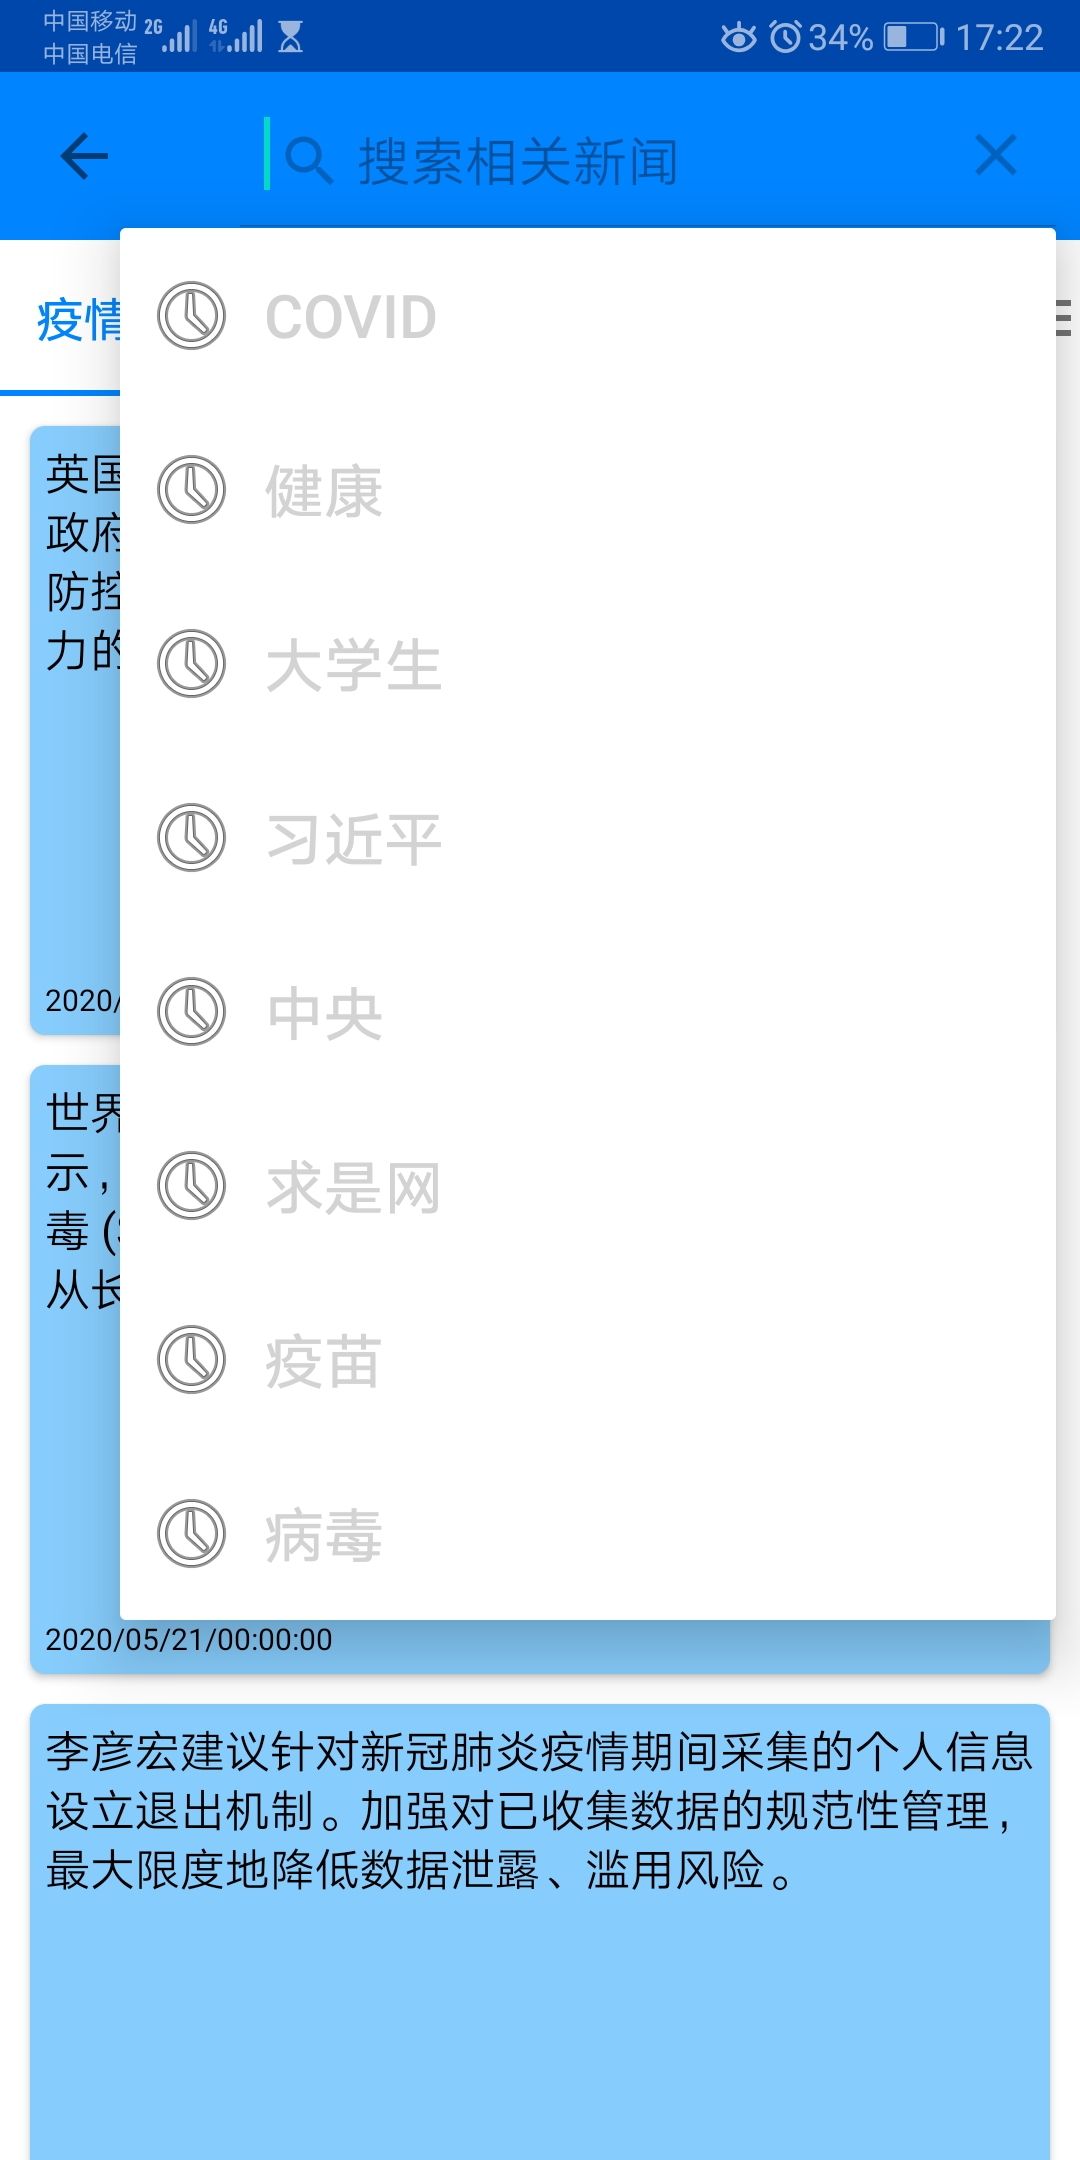
\includegraphics[width=0.8\textwidth]{search1}
        %\caption{fig2}
        \end{minipage}%
        }%
    \subfigure[搜索COVID页面]{
    \begin{minipage}[t]{0.3\linewidth}
    \centering
    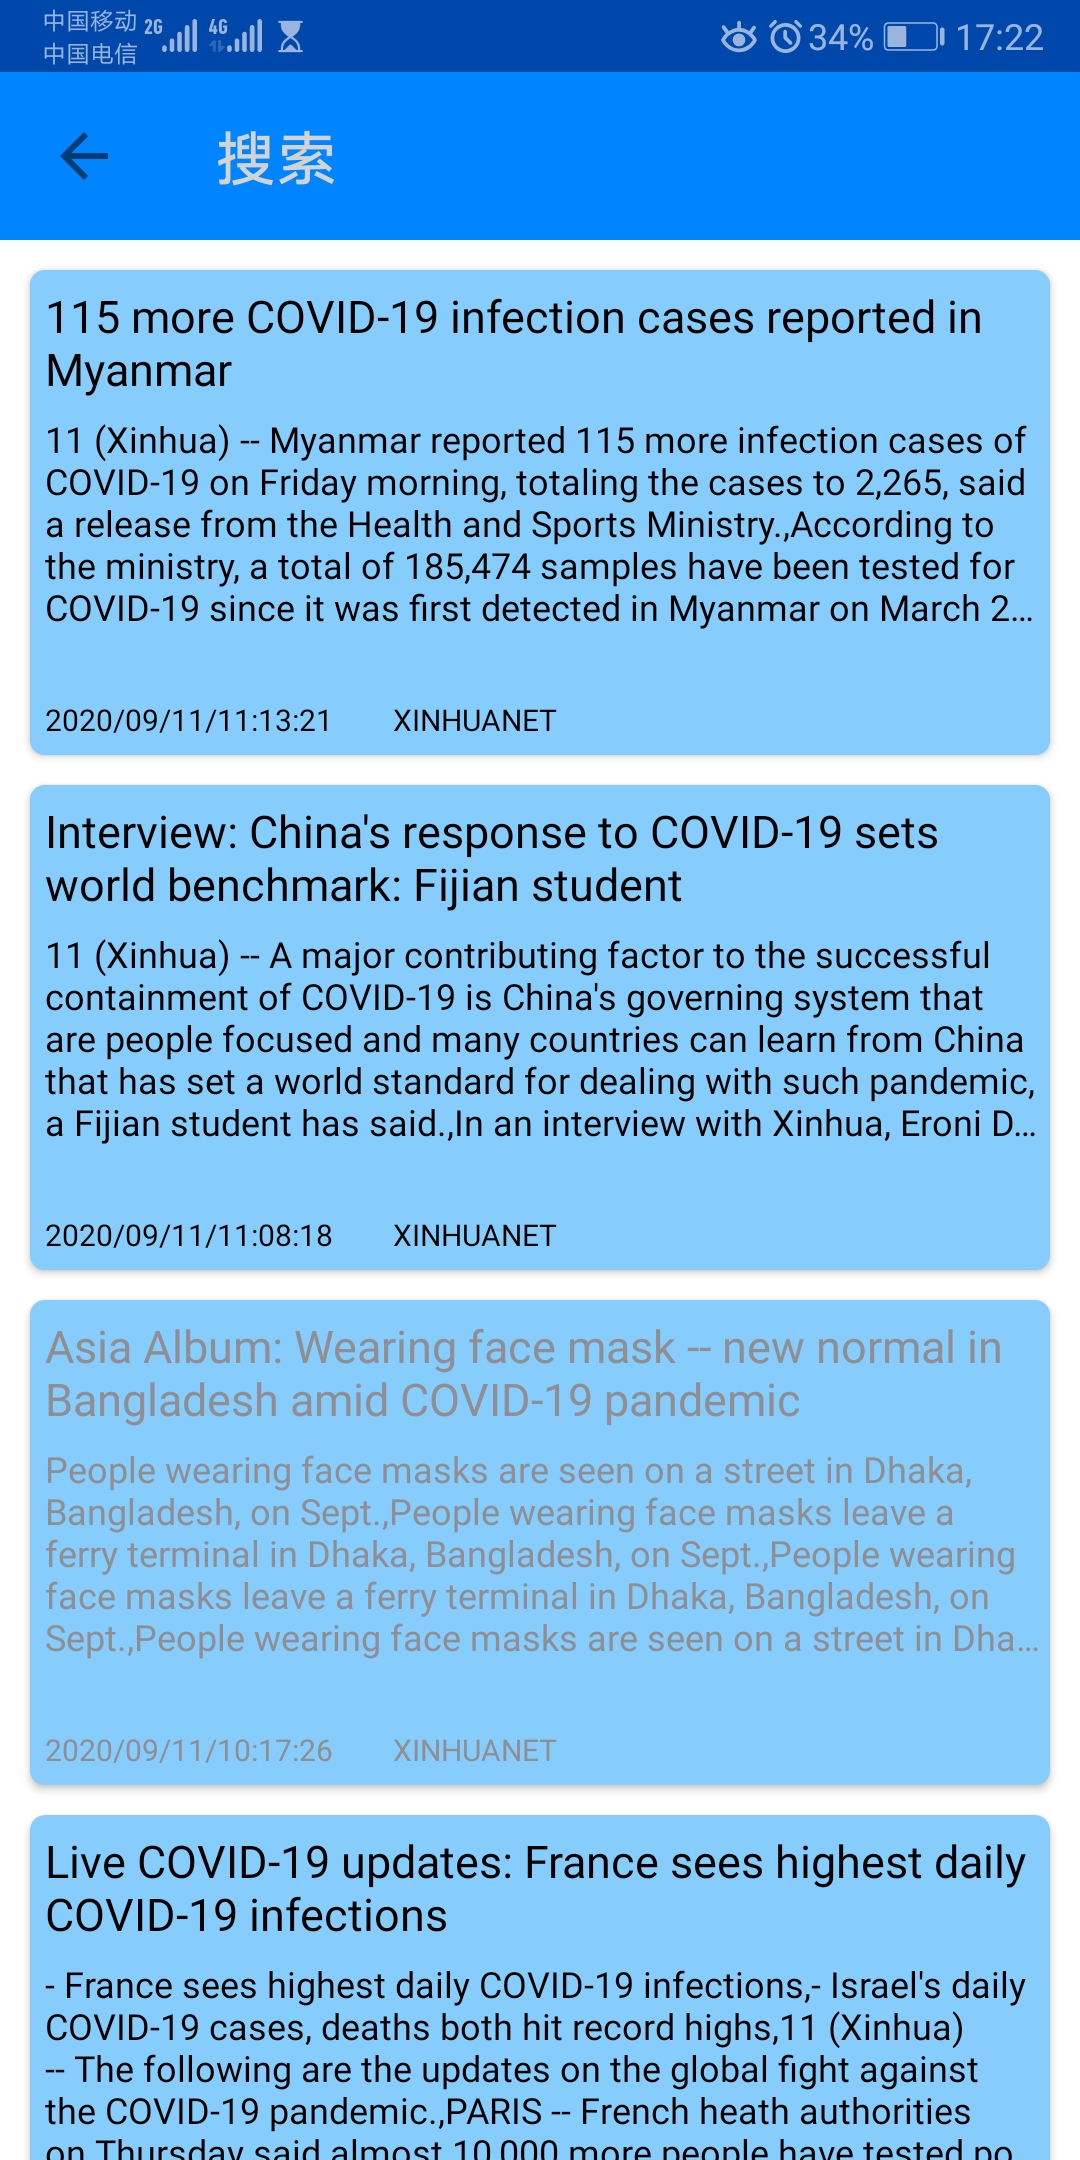
\includegraphics[width=0.8\textwidth]{search2}
    %\caption{fig1}
    \end{minipage}%
    }%
    \subfigure[搜索病毒页面]{
    \begin{minipage}[t]{0.3\linewidth}
    \centering
    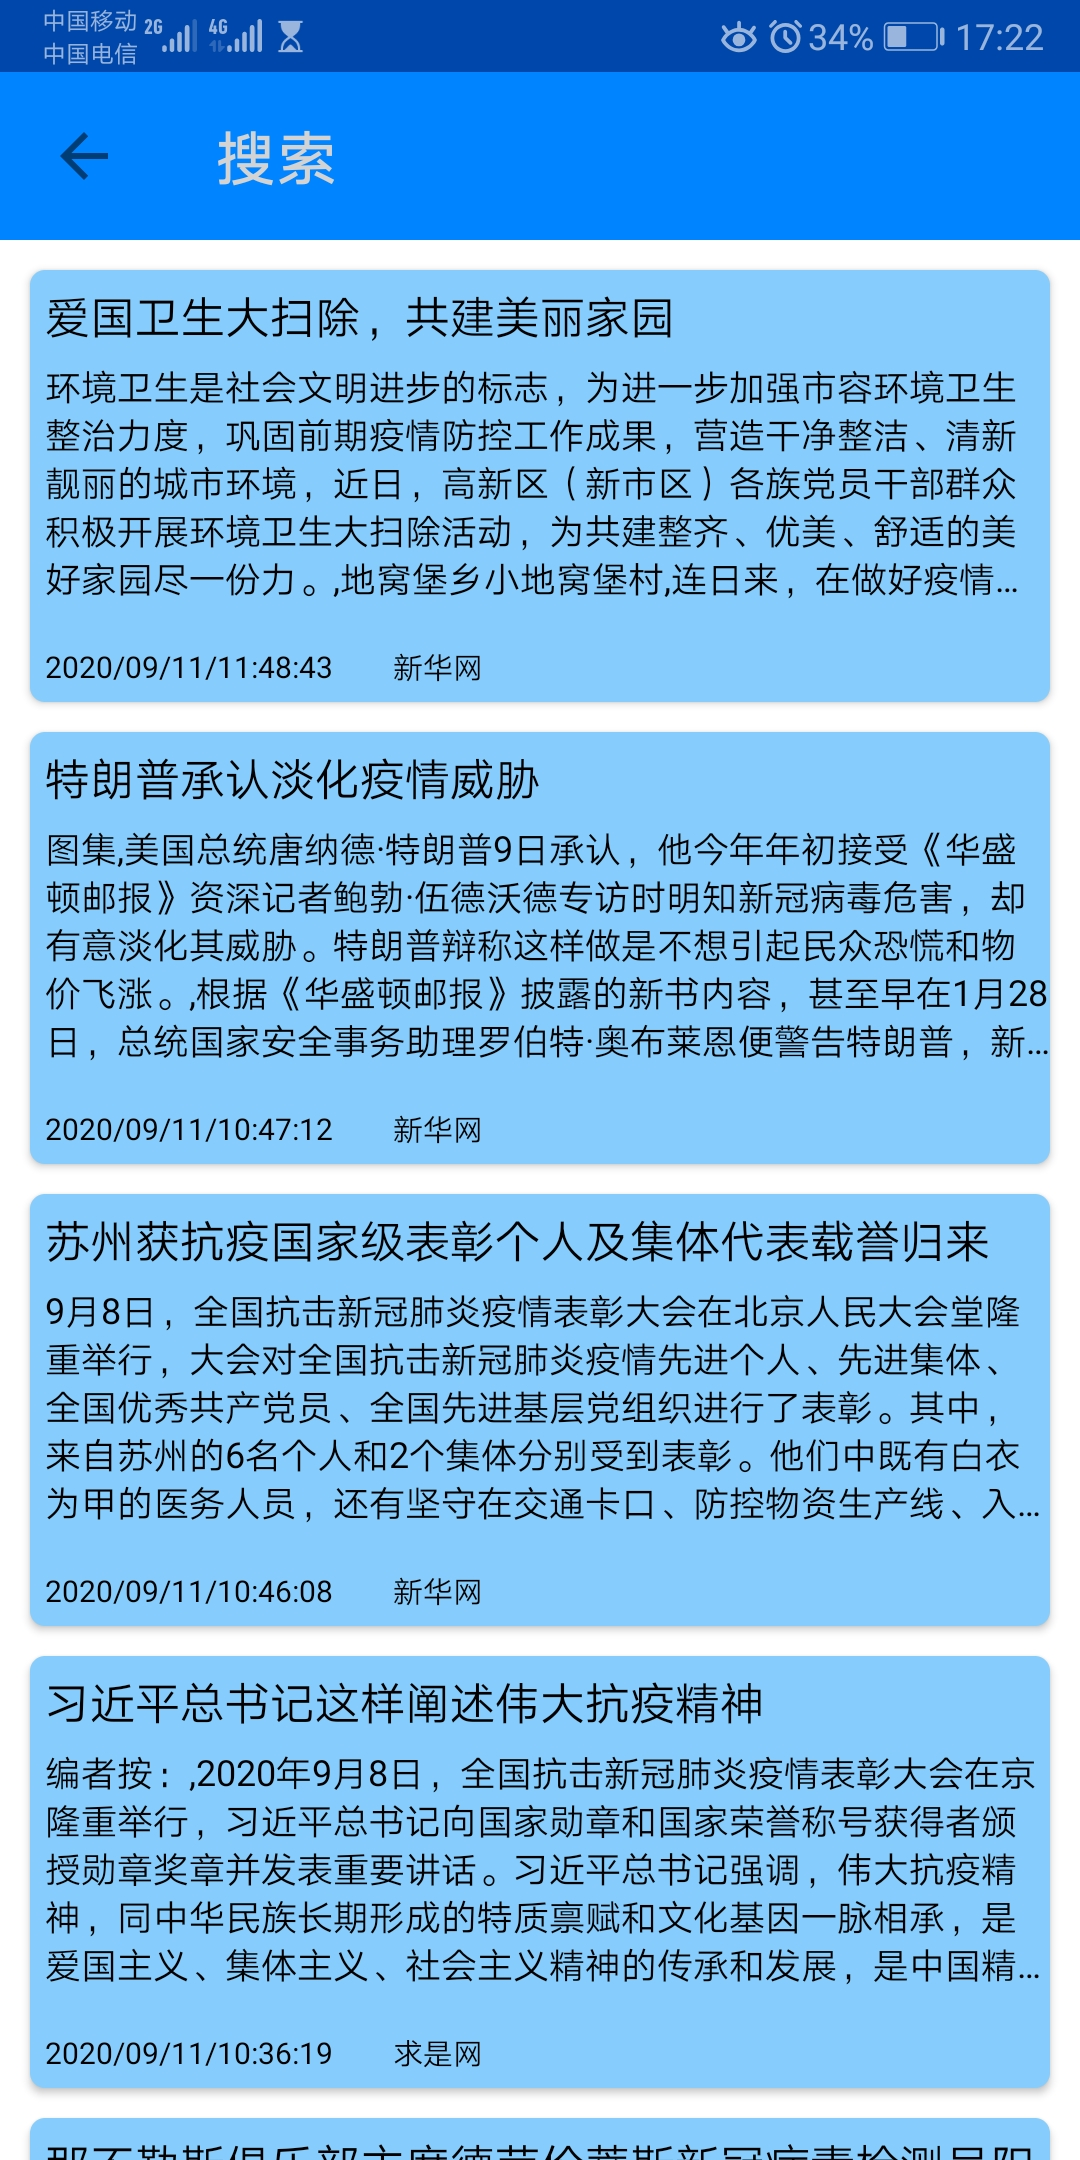
\includegraphics[width=0.8\textwidth]{search3}
    %\caption{fig2}
    \end{minipage}%
    }%

    \centering
    \caption{搜索结果页面}
    \end{figure}
% \clearpage
\subsubsection{新闻分享}
通过查看微信开发者文档,实现了基于WXWebPageObject的网页分享,能分享到用户好友。消息标题为新闻标题,消息内容为新闻摘要,消息url为对应的url。
值得注意的是微信要求摘要文字不能过长。
\begin{figure}[htbp]
    \centering
    \subfigure[分享到微信]{
    \begin{minipage}[t]{0.35\linewidth}
    \centering
    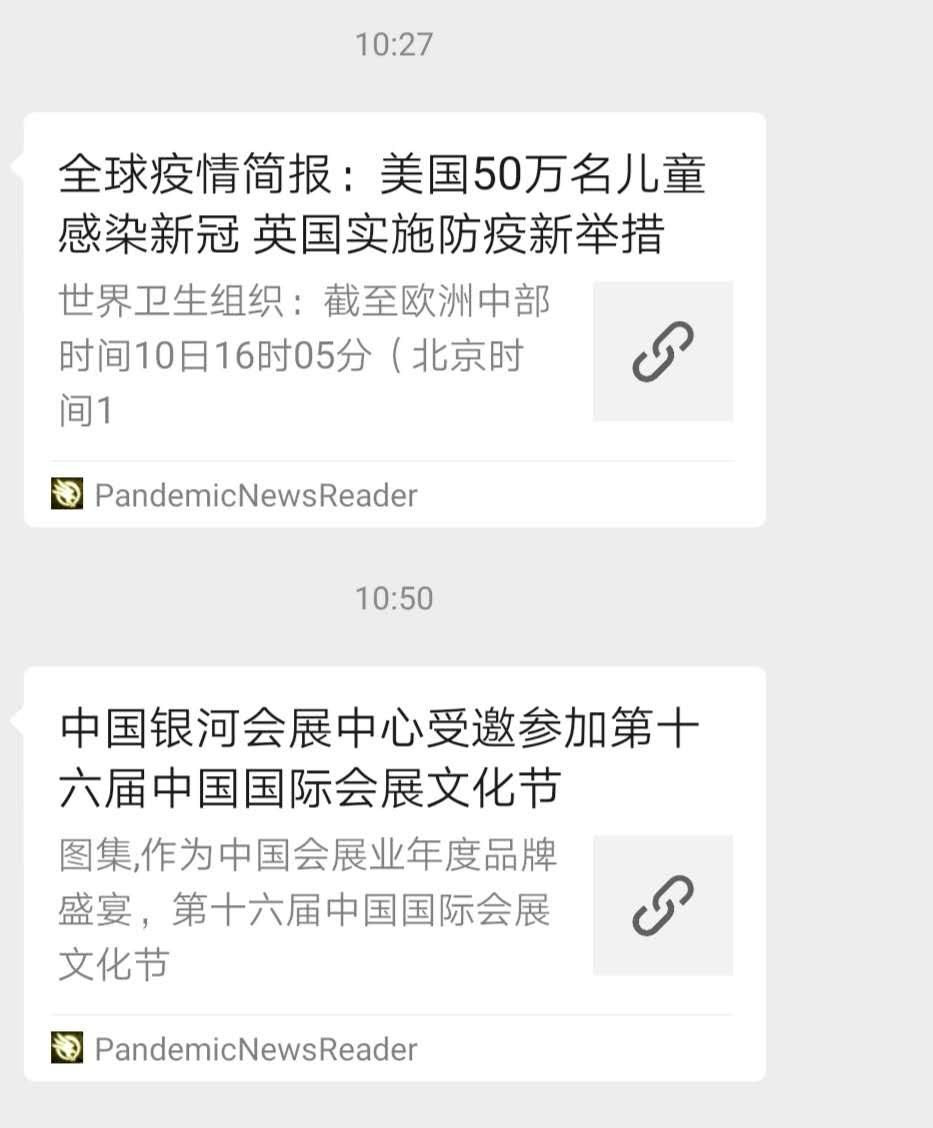
\includegraphics[width=0.7\textwidth]{share1}
    %\caption{fig1}
    \end{minipage}%
    }%
    \subfigure[点击打开后]{
    \begin{minipage}[t]{0.35\linewidth}
    \centering
    
\includegraphics[width=0.5\textwidth]{share2}
    %\caption{fig2}
    \end{minipage}%
    }%
    \centering
    \caption{分享结果页面}
    \end{figure}


\subsubsection{疫情数据展示}
疫情数据可视化我使用了第三方库MPAndroidChart,另外由于手机屏幕宽度的限制,全球疫情方面只显示了确诊人数前五的国家,用柱状图显示。
使用过程中发现MPAndroidChart的主要问题是没有提供修改显示图表坐标文字颜色的接口。

对于全国疫情,我参考了今日头条,使用了表格的形式进行展示。为了更方便地对表项进行定制,我没有使用TableLayout而是直接使用了RecyclerView。展示效果也令人满意。

在实现过程中,发现RecyclerView始终只展示第一个item,经过仔细比对后发现问题出在被我忽略的item的布局文件上,layout\_height属性应该取值为wrap\_content而非match\_parent。
容易理解,match\_parent会导致第一项直接占用全部的空间,遮挡住后续各项。

\begin{figure}[htbp]
    \centering
    \subfigure[国际疫情数据页面]{
    \begin{minipage}[t]{0.5\linewidth}
    \centering
    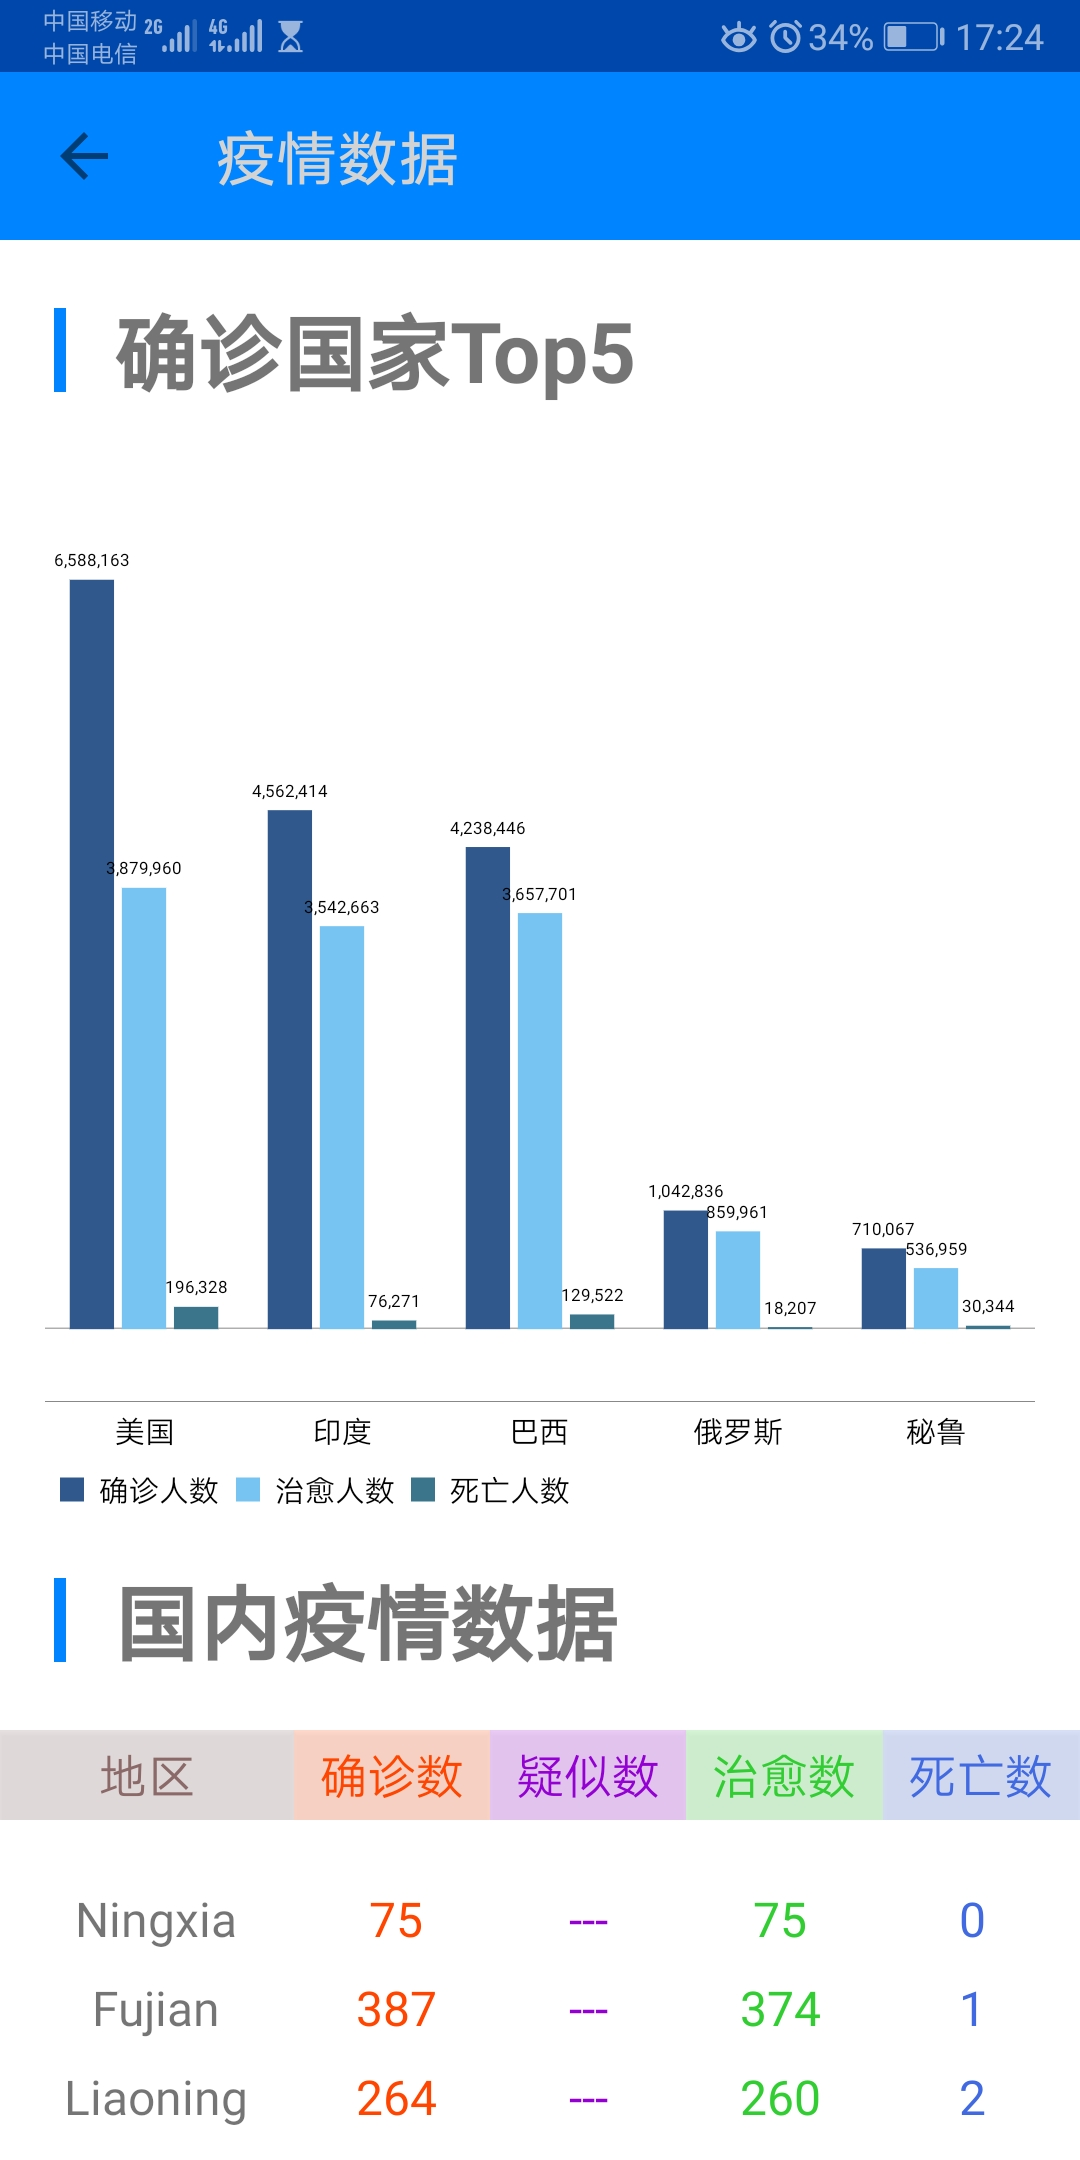
\includegraphics[width=0.5\textwidth]{dataview.jpg}
    %\caption{fig1}
    \end{minipage}%
    }%
    \subfigure[国内疫情数据界面]{
    \begin{minipage}[t]{0.5\linewidth}
    \centering
    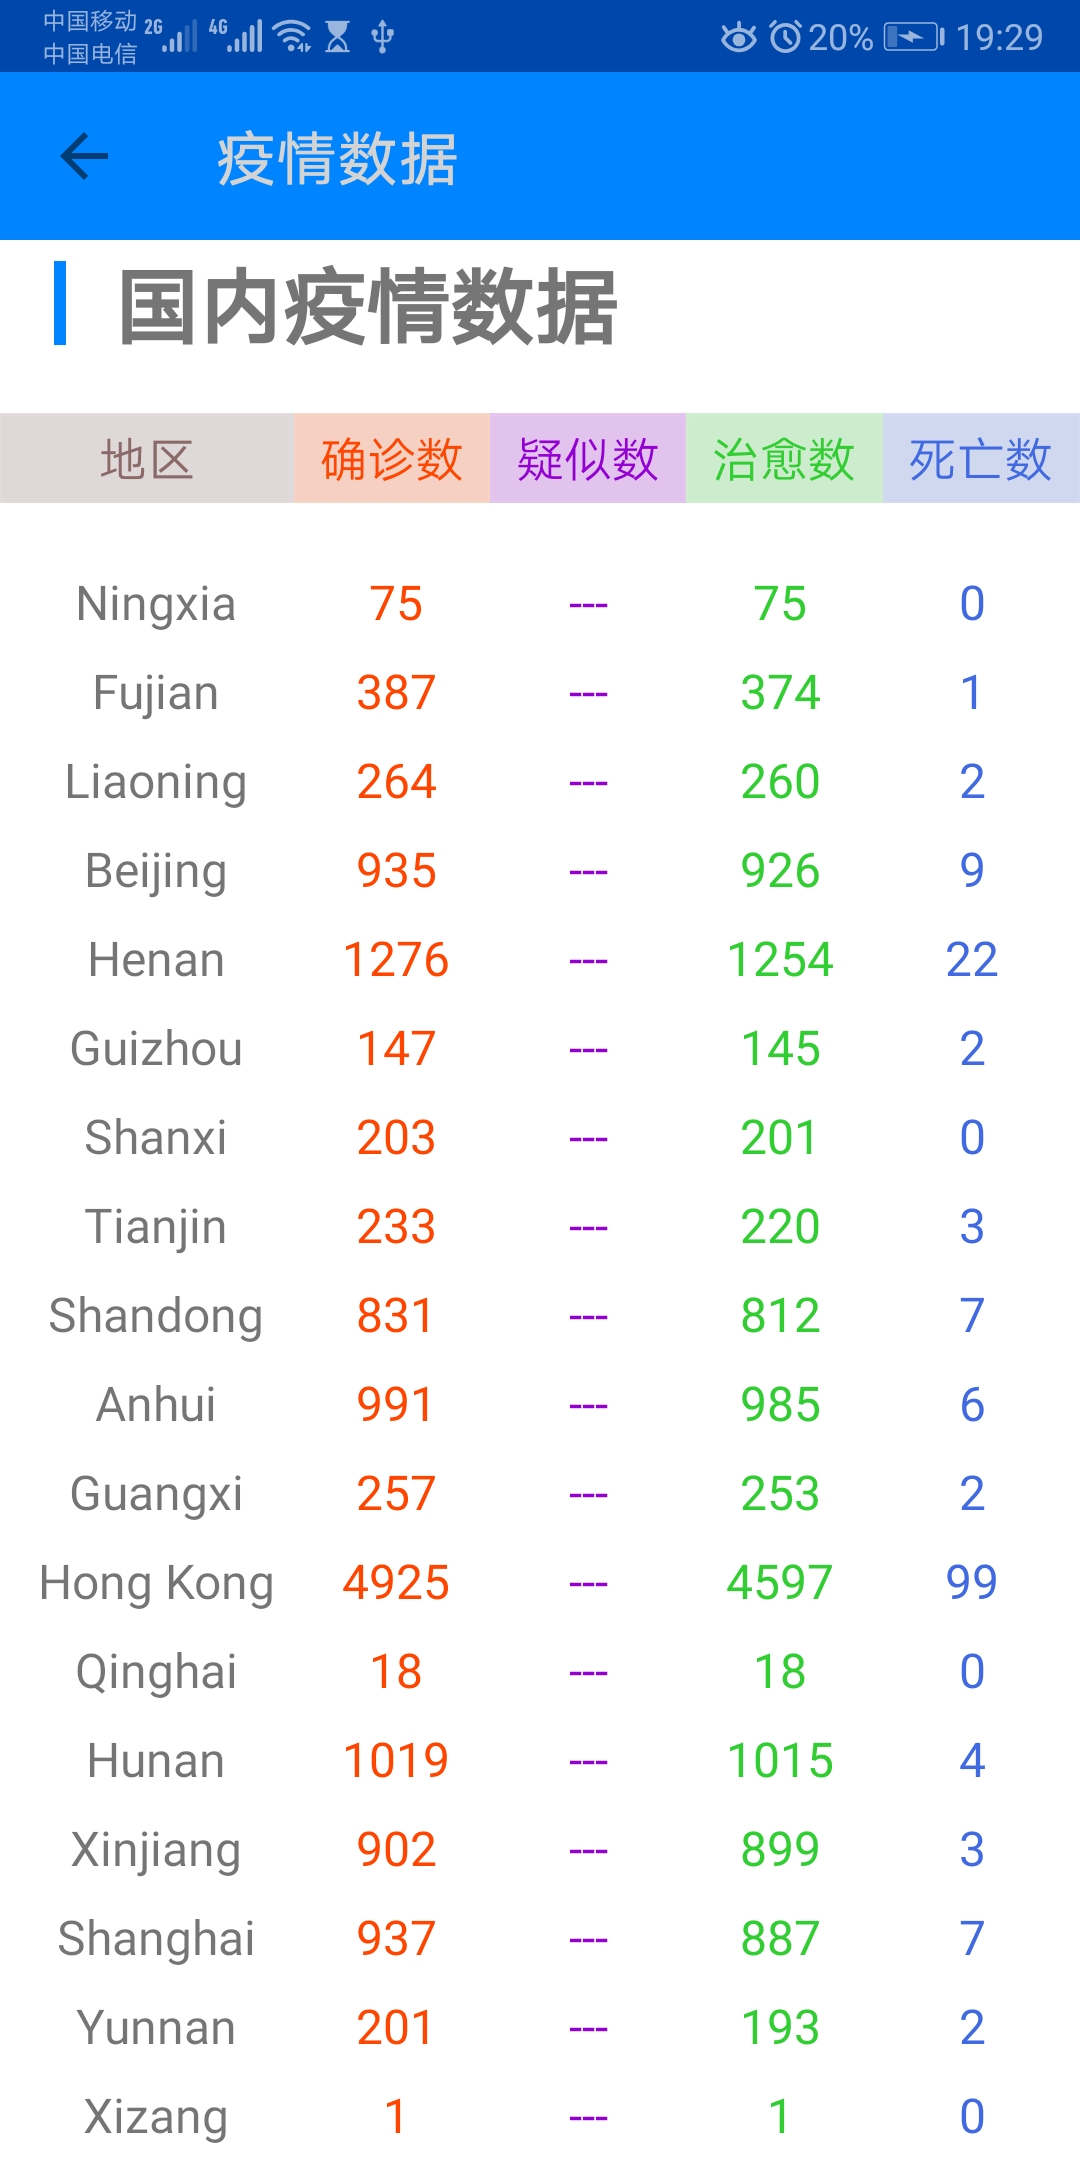
\includegraphics[width=0.5\textwidth]{dataview2.jpg}
    %\caption{fig2}
    \end{minipage}%
    }%
    \centering
    \caption{疫情数据界面}
    \end{figure}

% \begin{figure}[h]
%     \label{Ratio}
%     \centering
%         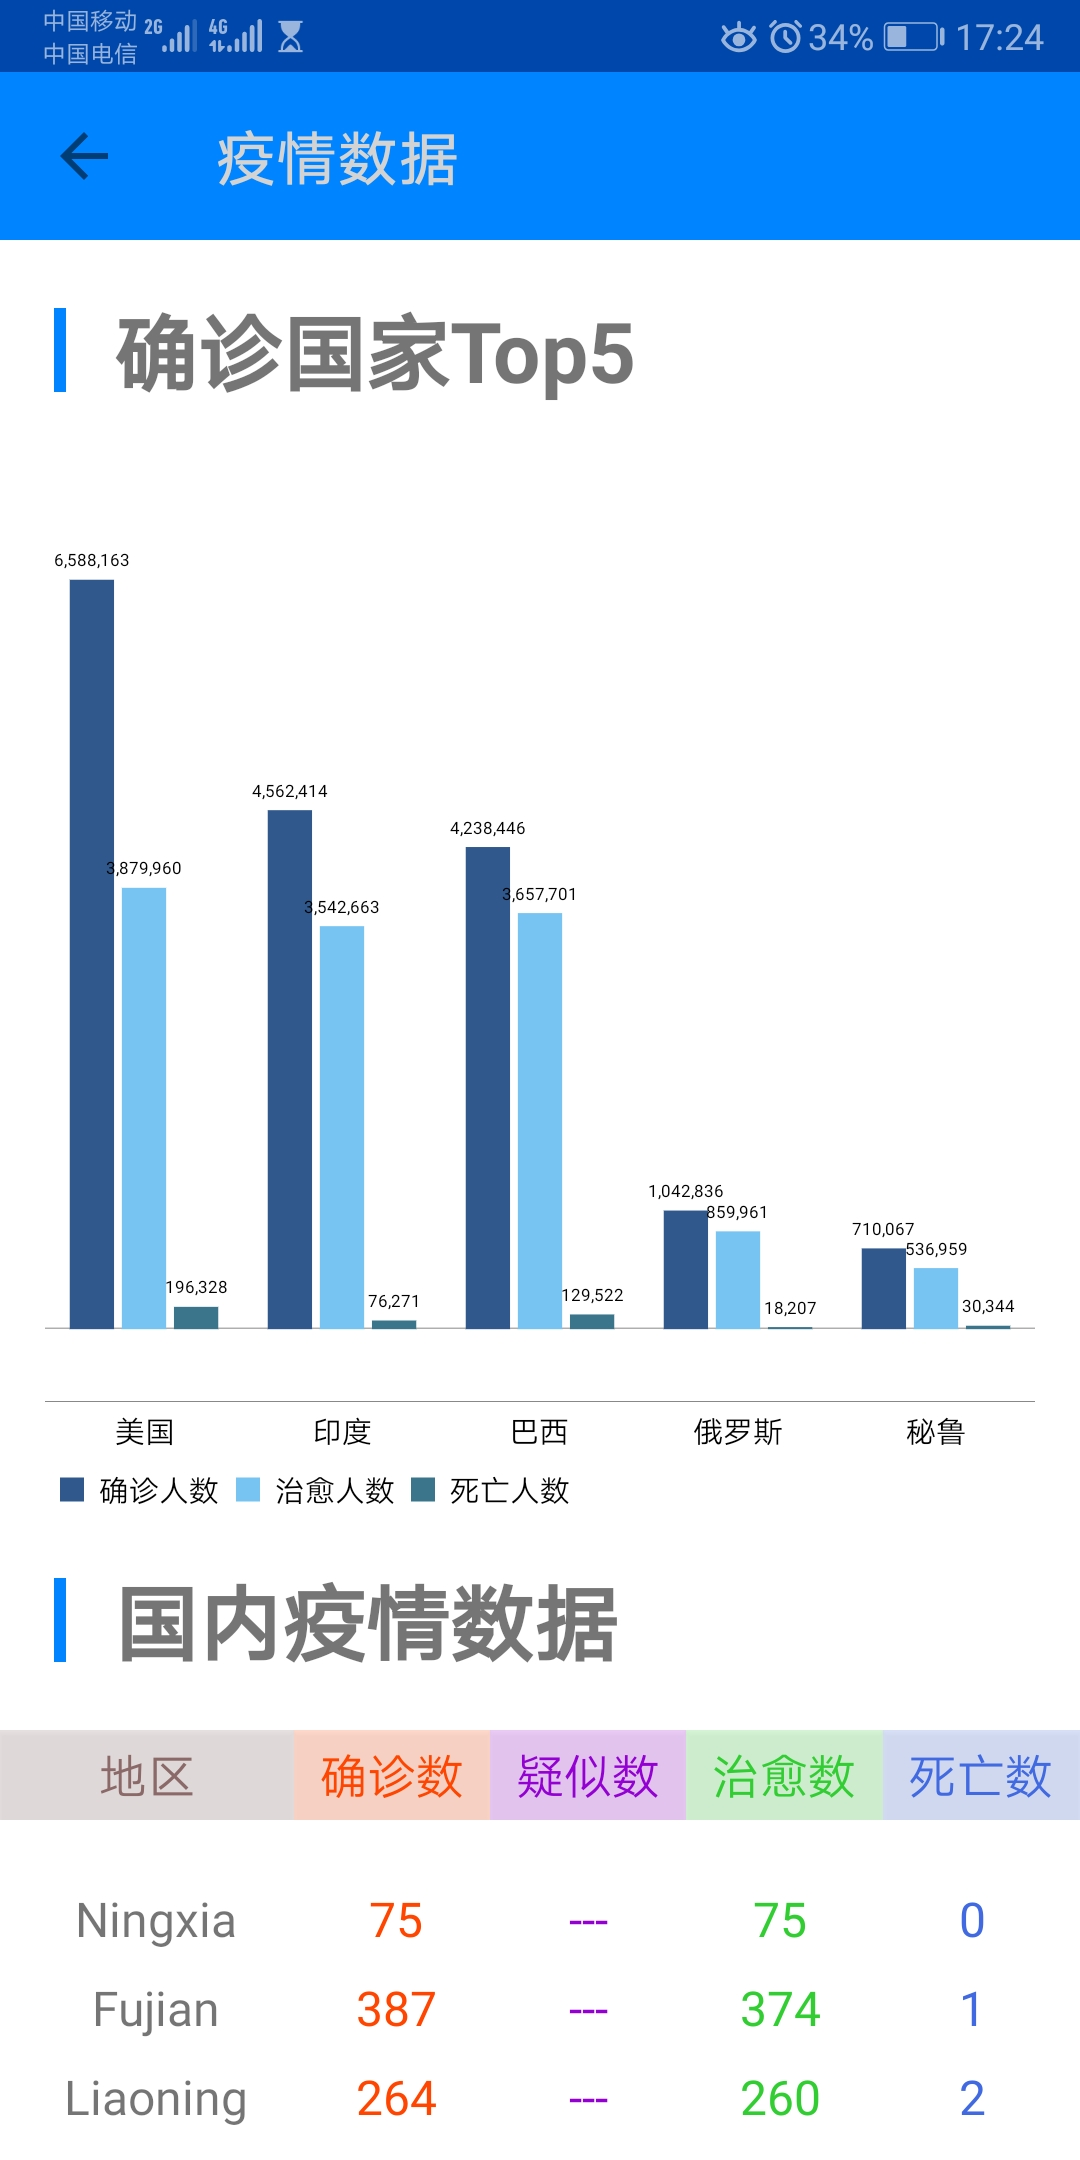
\includegraphics[height=0.5\textwidth]{dataview}
%         \caption{疫情数据页面}
%     \end{figure}

    \newpage
\subsubsection{疫情实体搜索}
本功能分为搜索和展示两个子功能。

搜索功能依然使用SearchView实现,由于发起搜索和展示在一个页面实现,有关的配置相反更简单了。这里不再赘述。

实体信息展示页面的实现花费了比较多的时间。这里我想实现类似于网页端的折叠与展开效果,最开始我的朴素想法是:RecyclerView的item布局里再嵌套一个RecyclerView?
但是经过一番搜索后发现这样实现的性能会出大问题(RecyclerView本身的性能就可能随着项数的增多而降低,如果采取多层RecyclerView嵌套的方式实现,不仅会出现滑动错乱的问题,
还可能会导致页面卡顿,影响使用体验),推荐的做法是只使用一层RecyclerView实现展开效果,将不同级的项在代码中“视为”同一级,只不过通过展开和隐藏的方式响应点击事件。

另外我想到多级折叠展开效果在安卓中其实非常常见,比如我们熟悉的文件管理器。这实质上就是一种树形结构。通过这些关键词的搜索,我找到了一个实现简洁、文档易理解的第三方库:TreeView。
这个库的使用人数实在太少,因此网上根本没有对应的教程。我通过查看该库的源码后发现,使用该库需要自定义每层的ViewBinder用于绑定每层布局所需要的数据。但该控件不支持单一ViewBinder绑定多个布局文件,
这不符合本处第三级展开时布局不同的要求。在第三级展开中,描述/关系/属性三级对应的布局肯定是不同的,但是又只能包含在同一个布局中。上课时老师介绍过FrameLayout默认情况下会导致重叠效果,
我觉得正好能够实现本处需求:通过一个FrameLayout包裹三个不同的布局,并通过java代码设置它们是否可见。

由于RecyclerView计算高度并移动item相对耗时,而返回的实体信息中某些热门实体如“药物”的关系非常之多,而大部分实体的关系比较少,因此前端截取了前20条(如果大于20条)关系进行展示,
以免造成应用的性能问题。

\begin{figure}[htbp]
    \centering
    \subfigure[实体搜索页面(尚未搜索时)]{
        \begin{minipage}[t]{0.25\linewidth}
        \centering
        
\includegraphics[width=0.8\textwidth]{searchentity1}
        %\caption{fig2}
        \end{minipage}%
        }%
    \subfigure[一级展开]{
        \begin{minipage}[t]{0.25\linewidth}
        \centering
        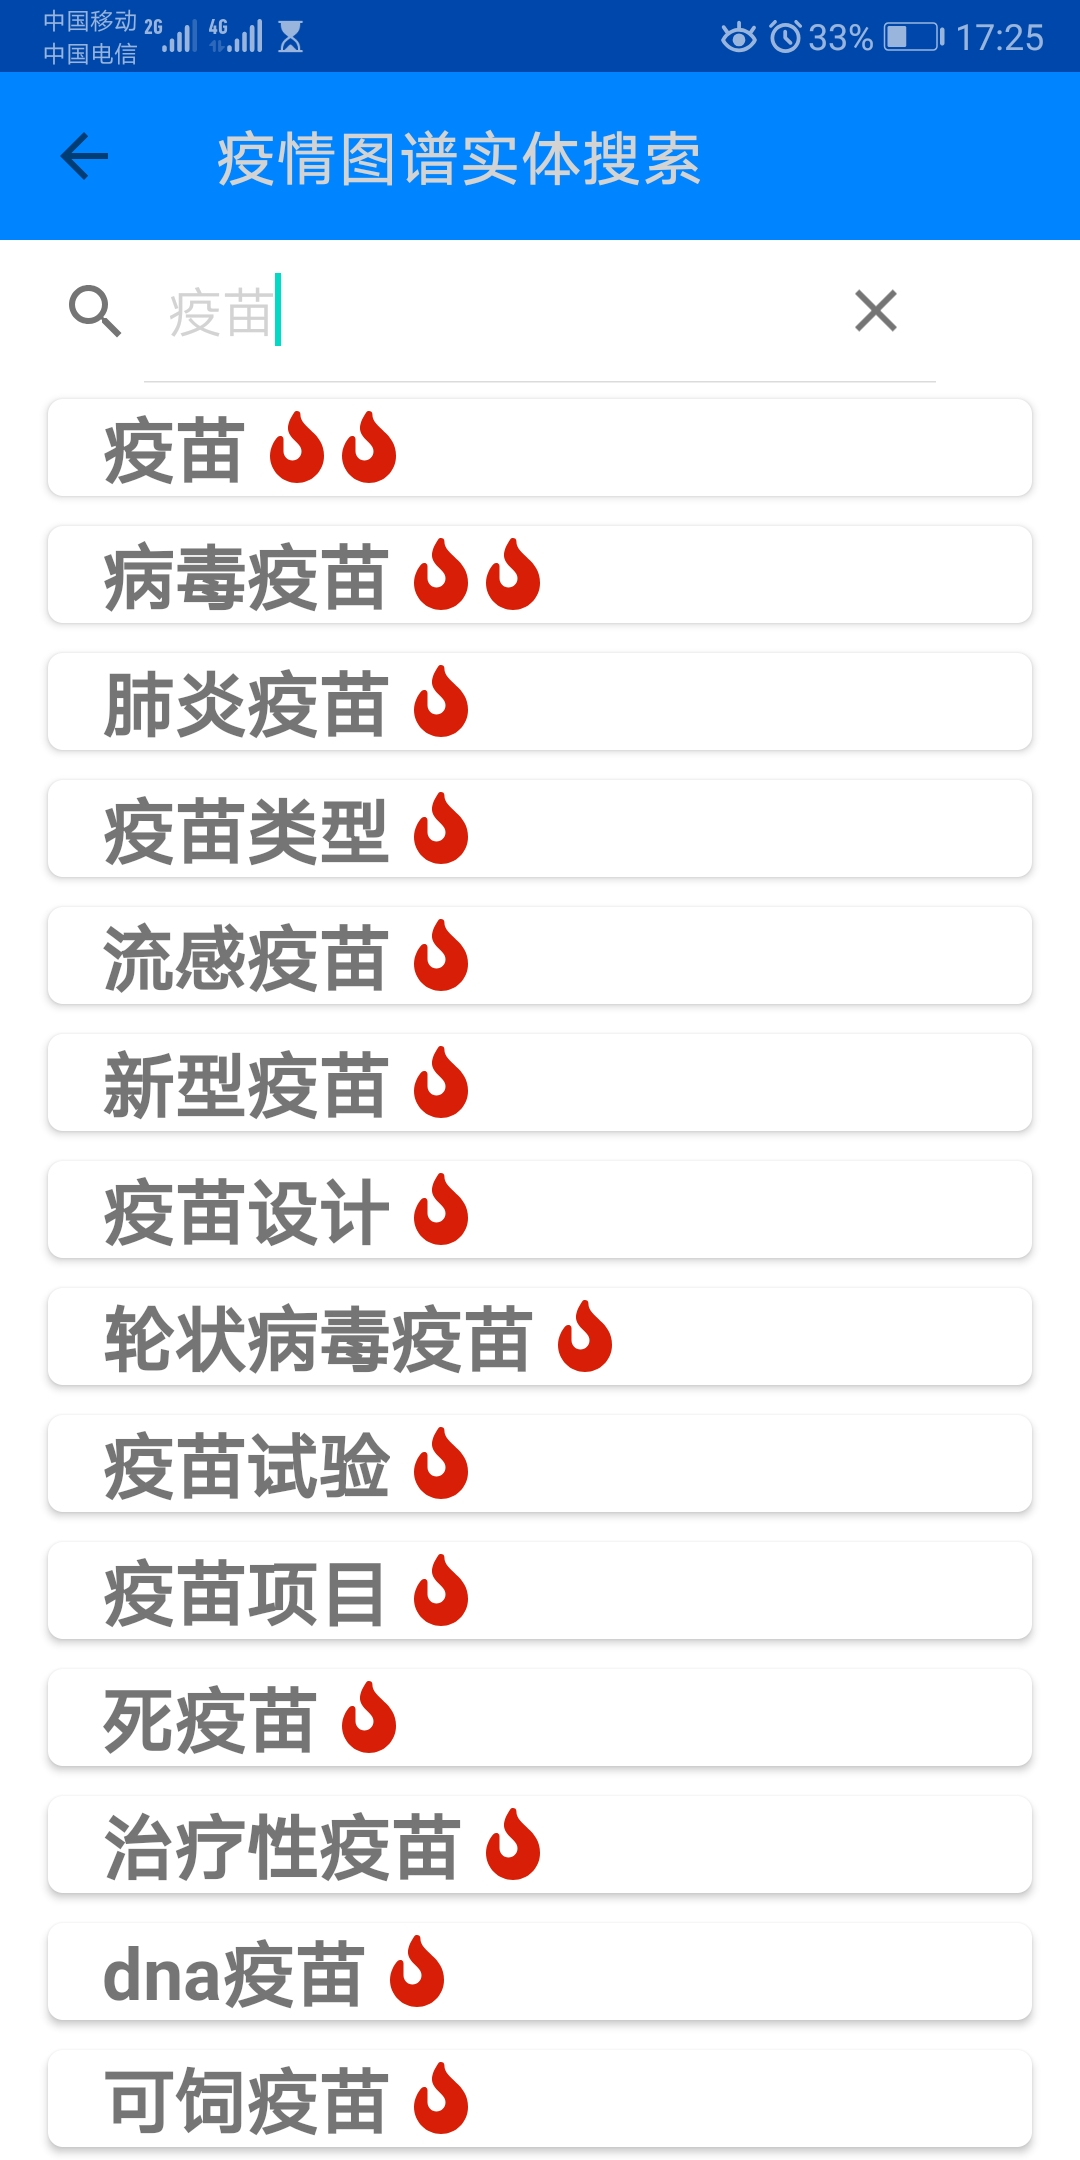
\includegraphics[width=0.8\textwidth]{searchentity2}
        %\caption{fig2}
        \end{minipage}%
        }%
    \subfigure[二级展开]{
    \begin{minipage}[t]{0.25\linewidth}
    \centering
    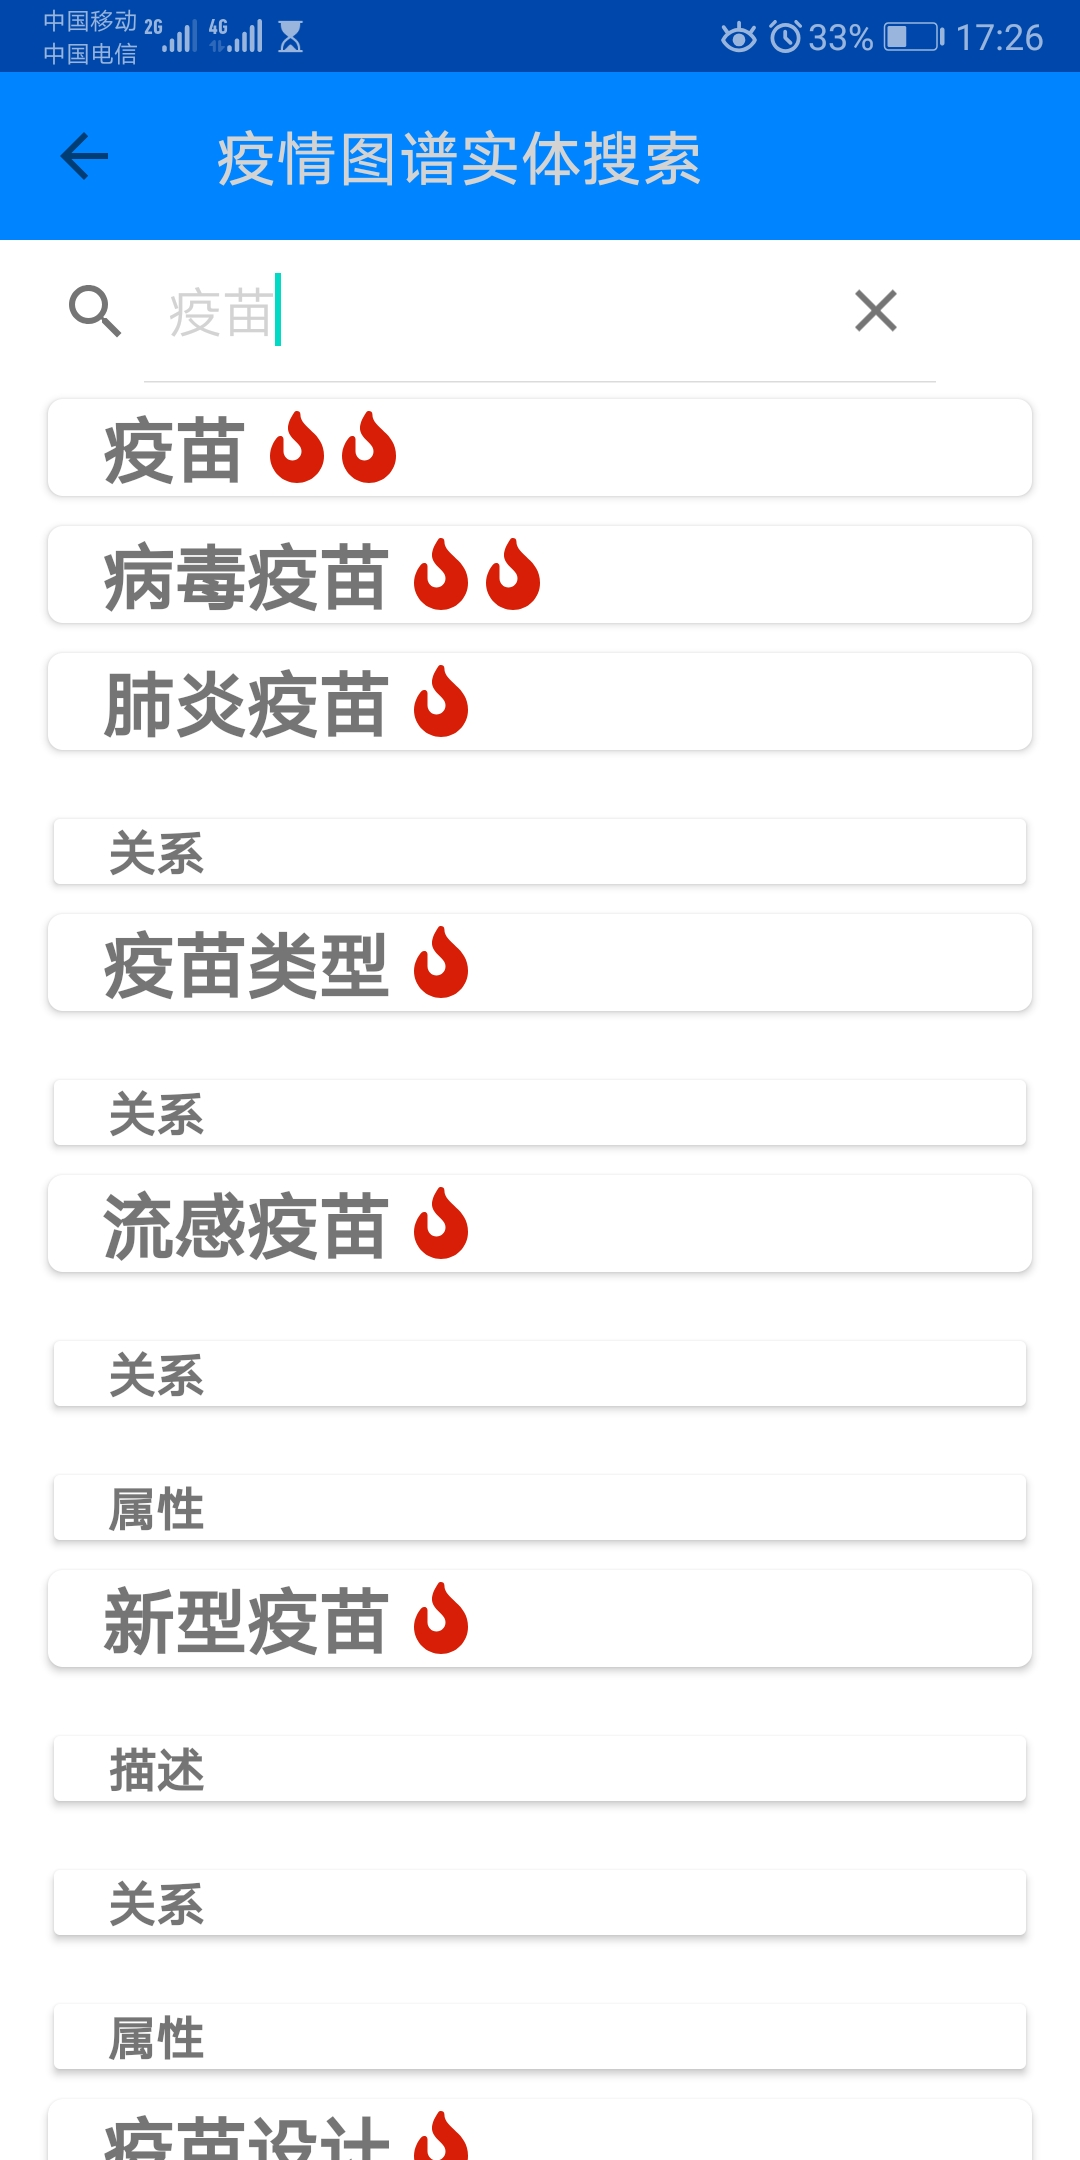
\includegraphics[width=0.8\textwidth]{searchentity3}
    %\caption{fig1}
    \end{minipage}%
    }%
    \subfigure[三级展开]{
    \begin{minipage}[t]{0.25\linewidth}
    \centering
    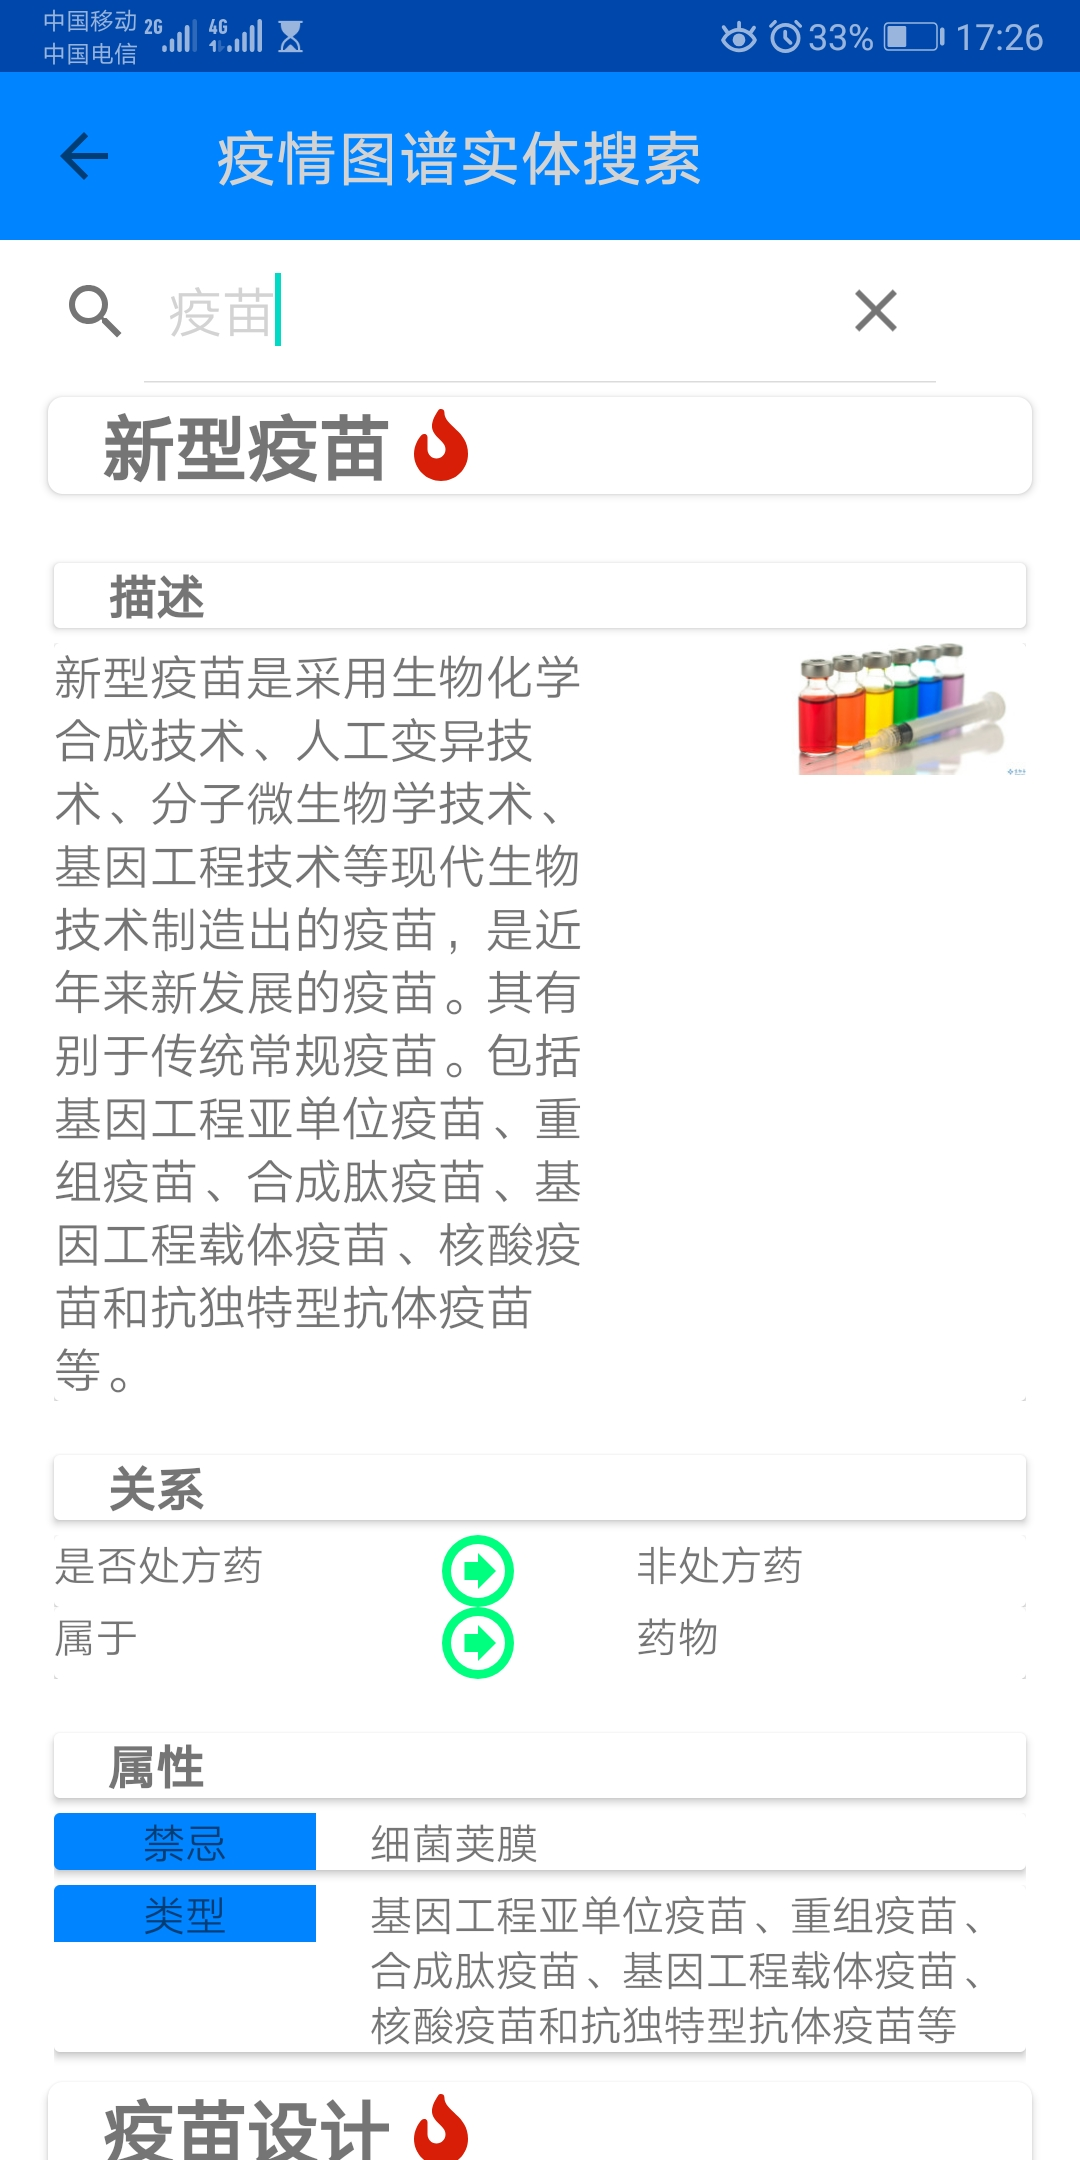
\includegraphics[width=0.8\textwidth]{searchentity4}
    %\caption{fig2}
    \end{minipage}%
    }%

    \centering
    \caption{搜索结果页面}
    \end{figure}


% \begin{figure}[h]
%     \centering
%     \subfigure[实体搜索页面(尚未搜索时)]{
%     
\includegraphics[width=5.5cm]{searchentity1}
%     }
%     \quad
%     \subfigure[一级展开]{
%     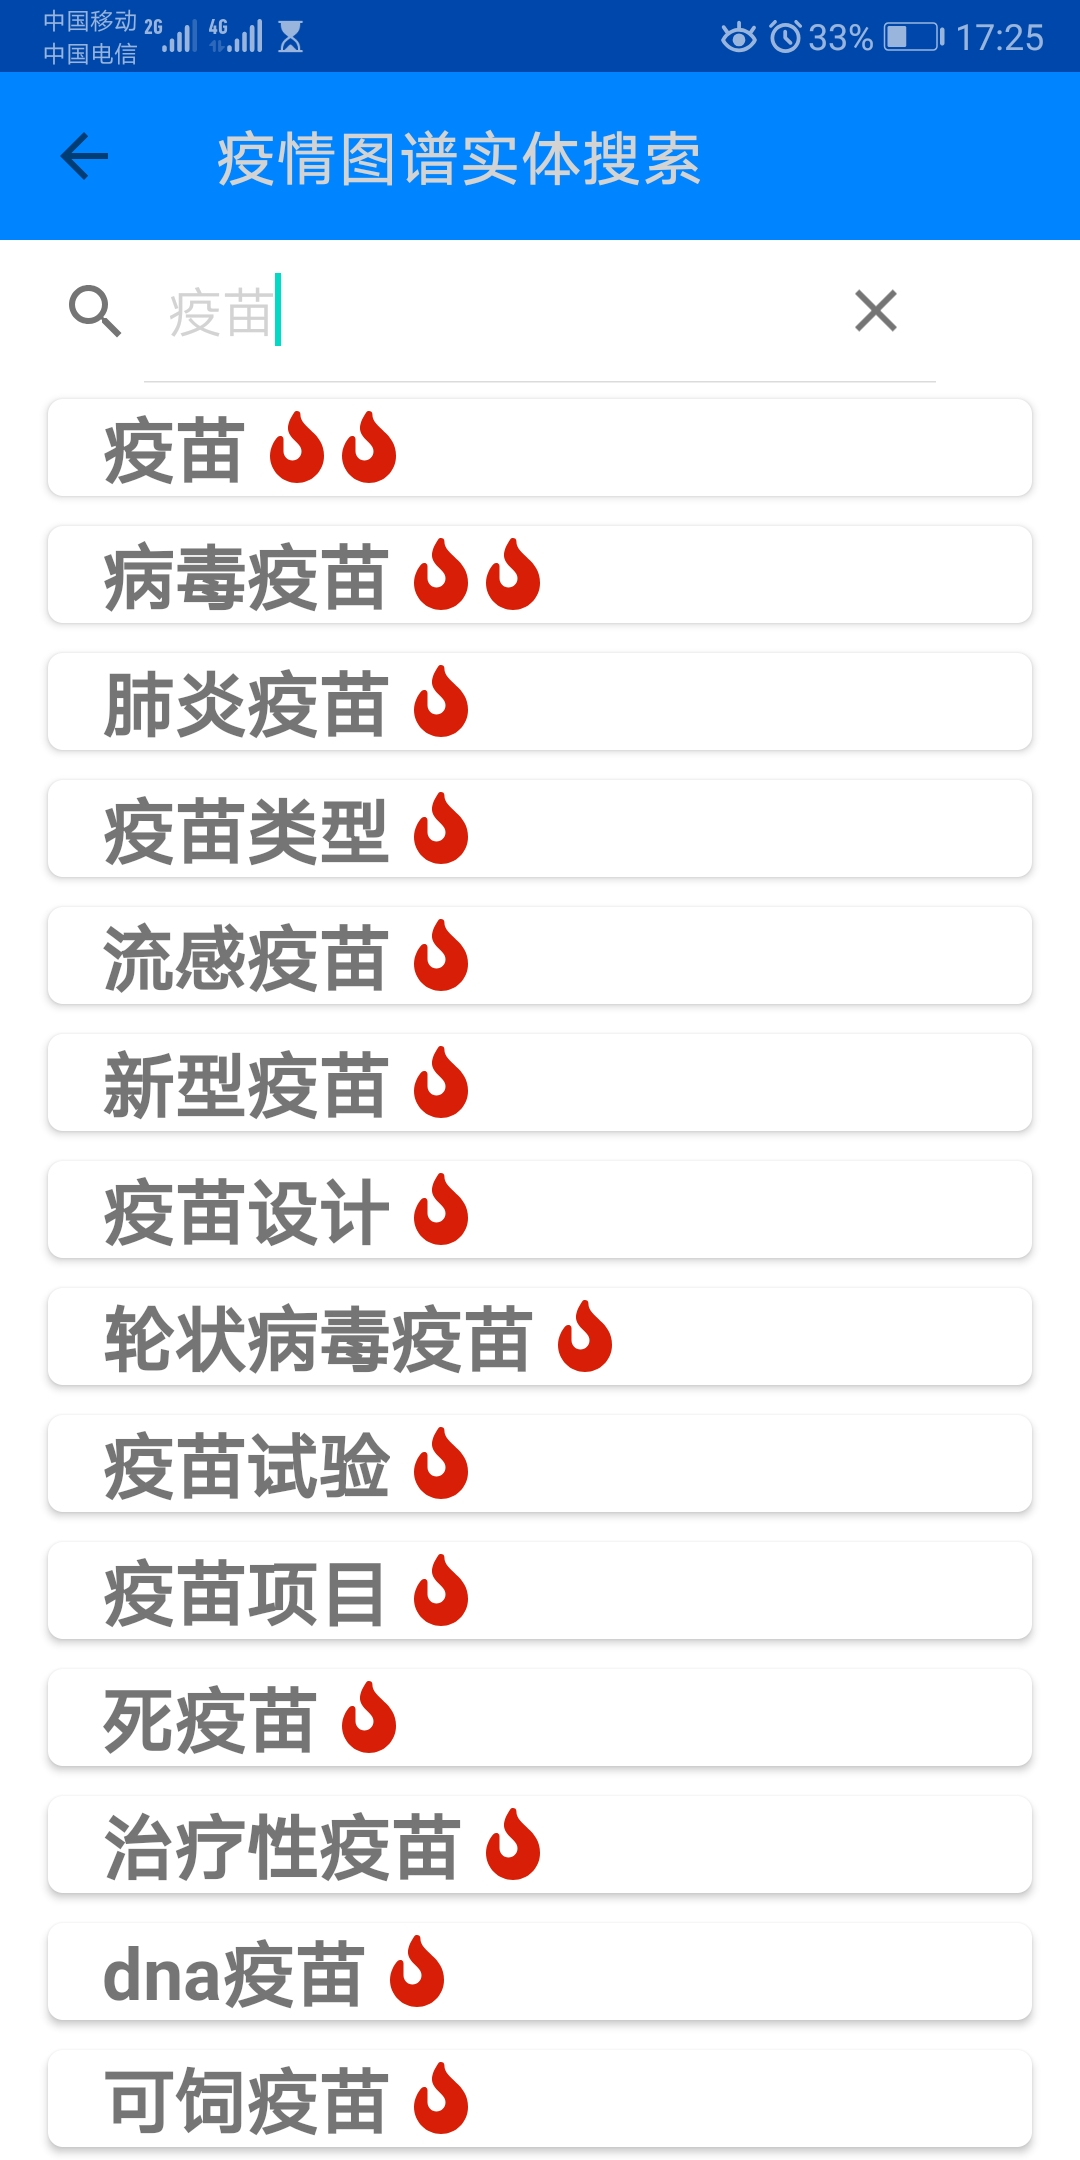
\includegraphics[width=5.5cm]{searchentity2}
%     }
%     \quad
%     \subfigure[二级展开]{
%     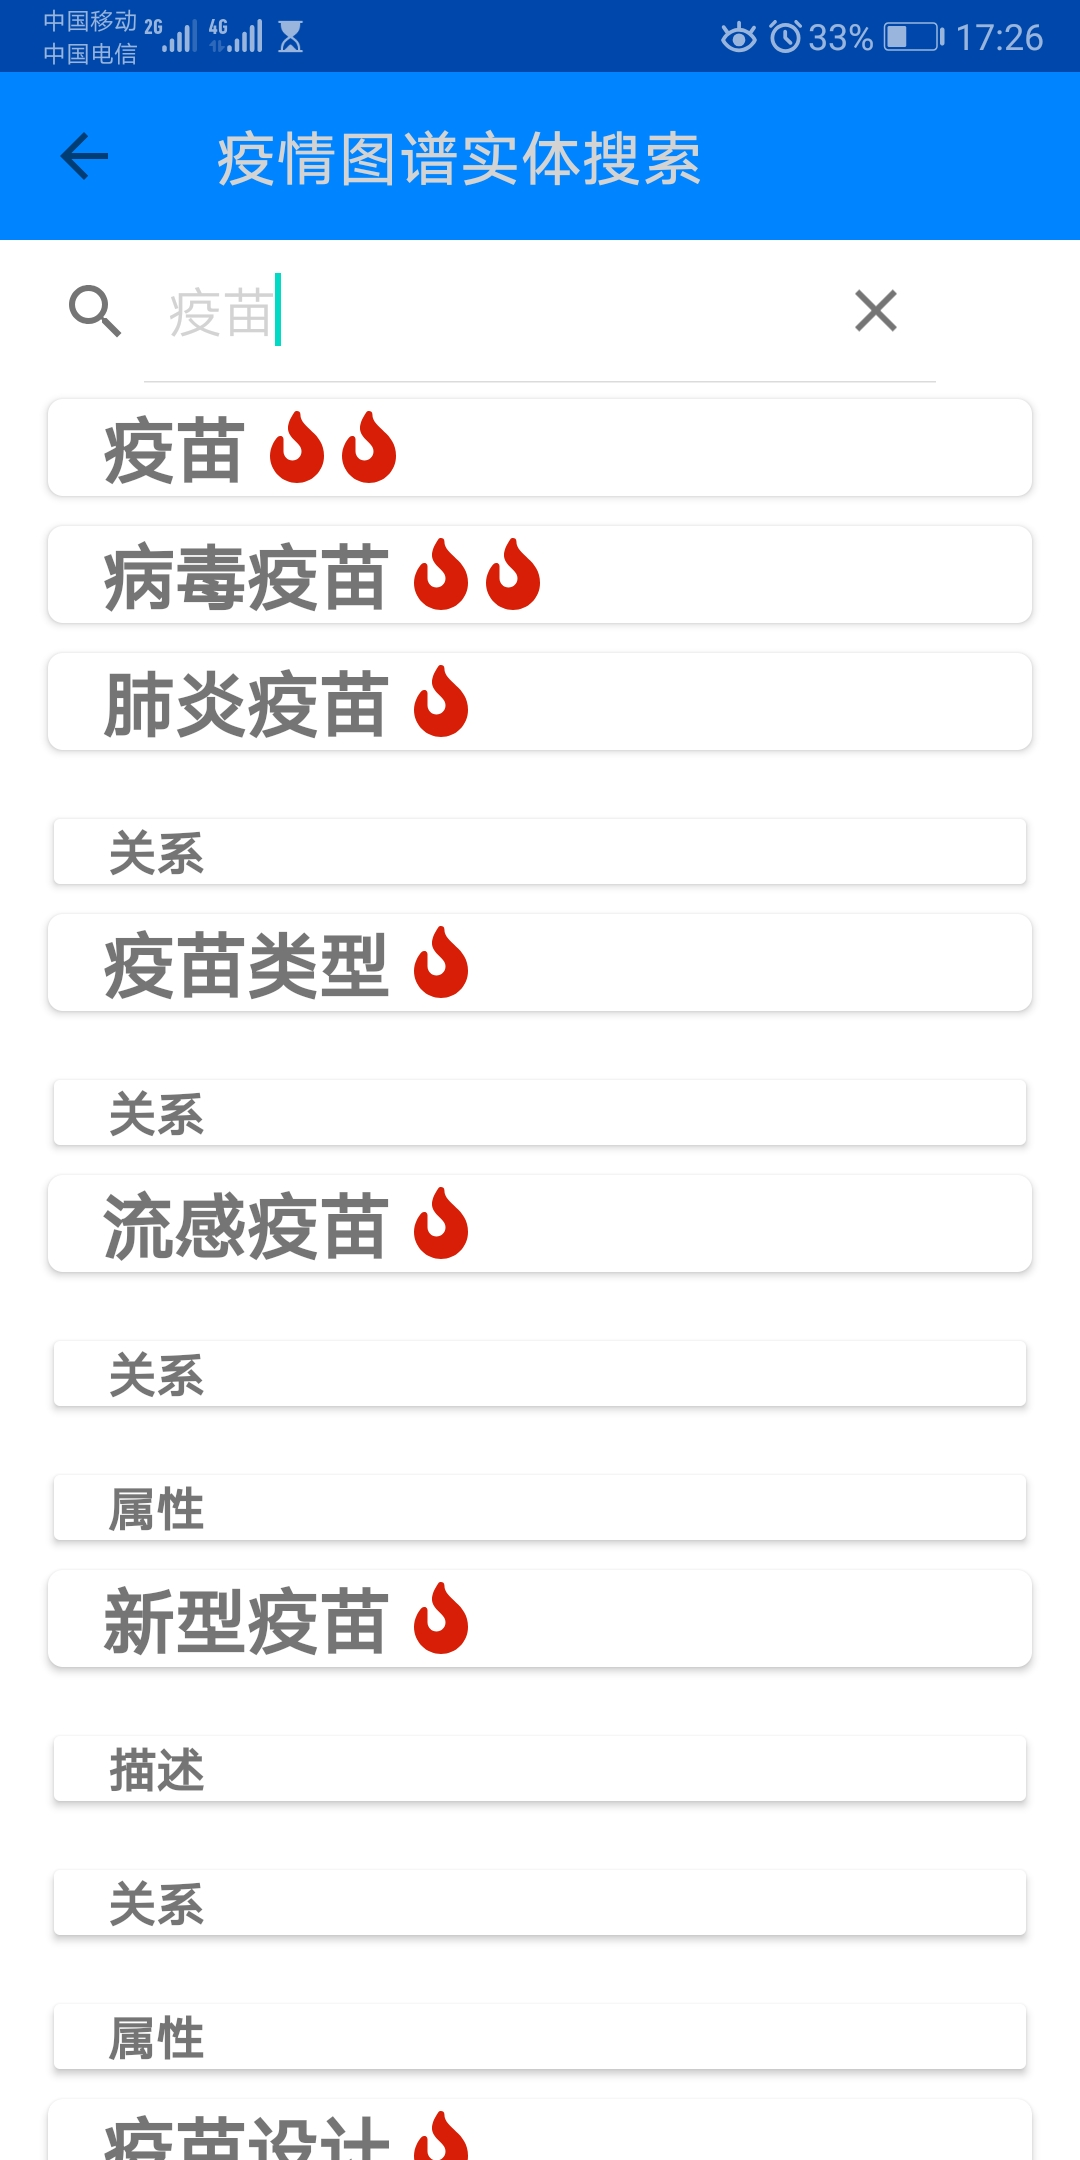
\includegraphics[width=5.5cm]{searchentity3}
%     }
%     \quad
%     \subfigure[三级展开]{
%     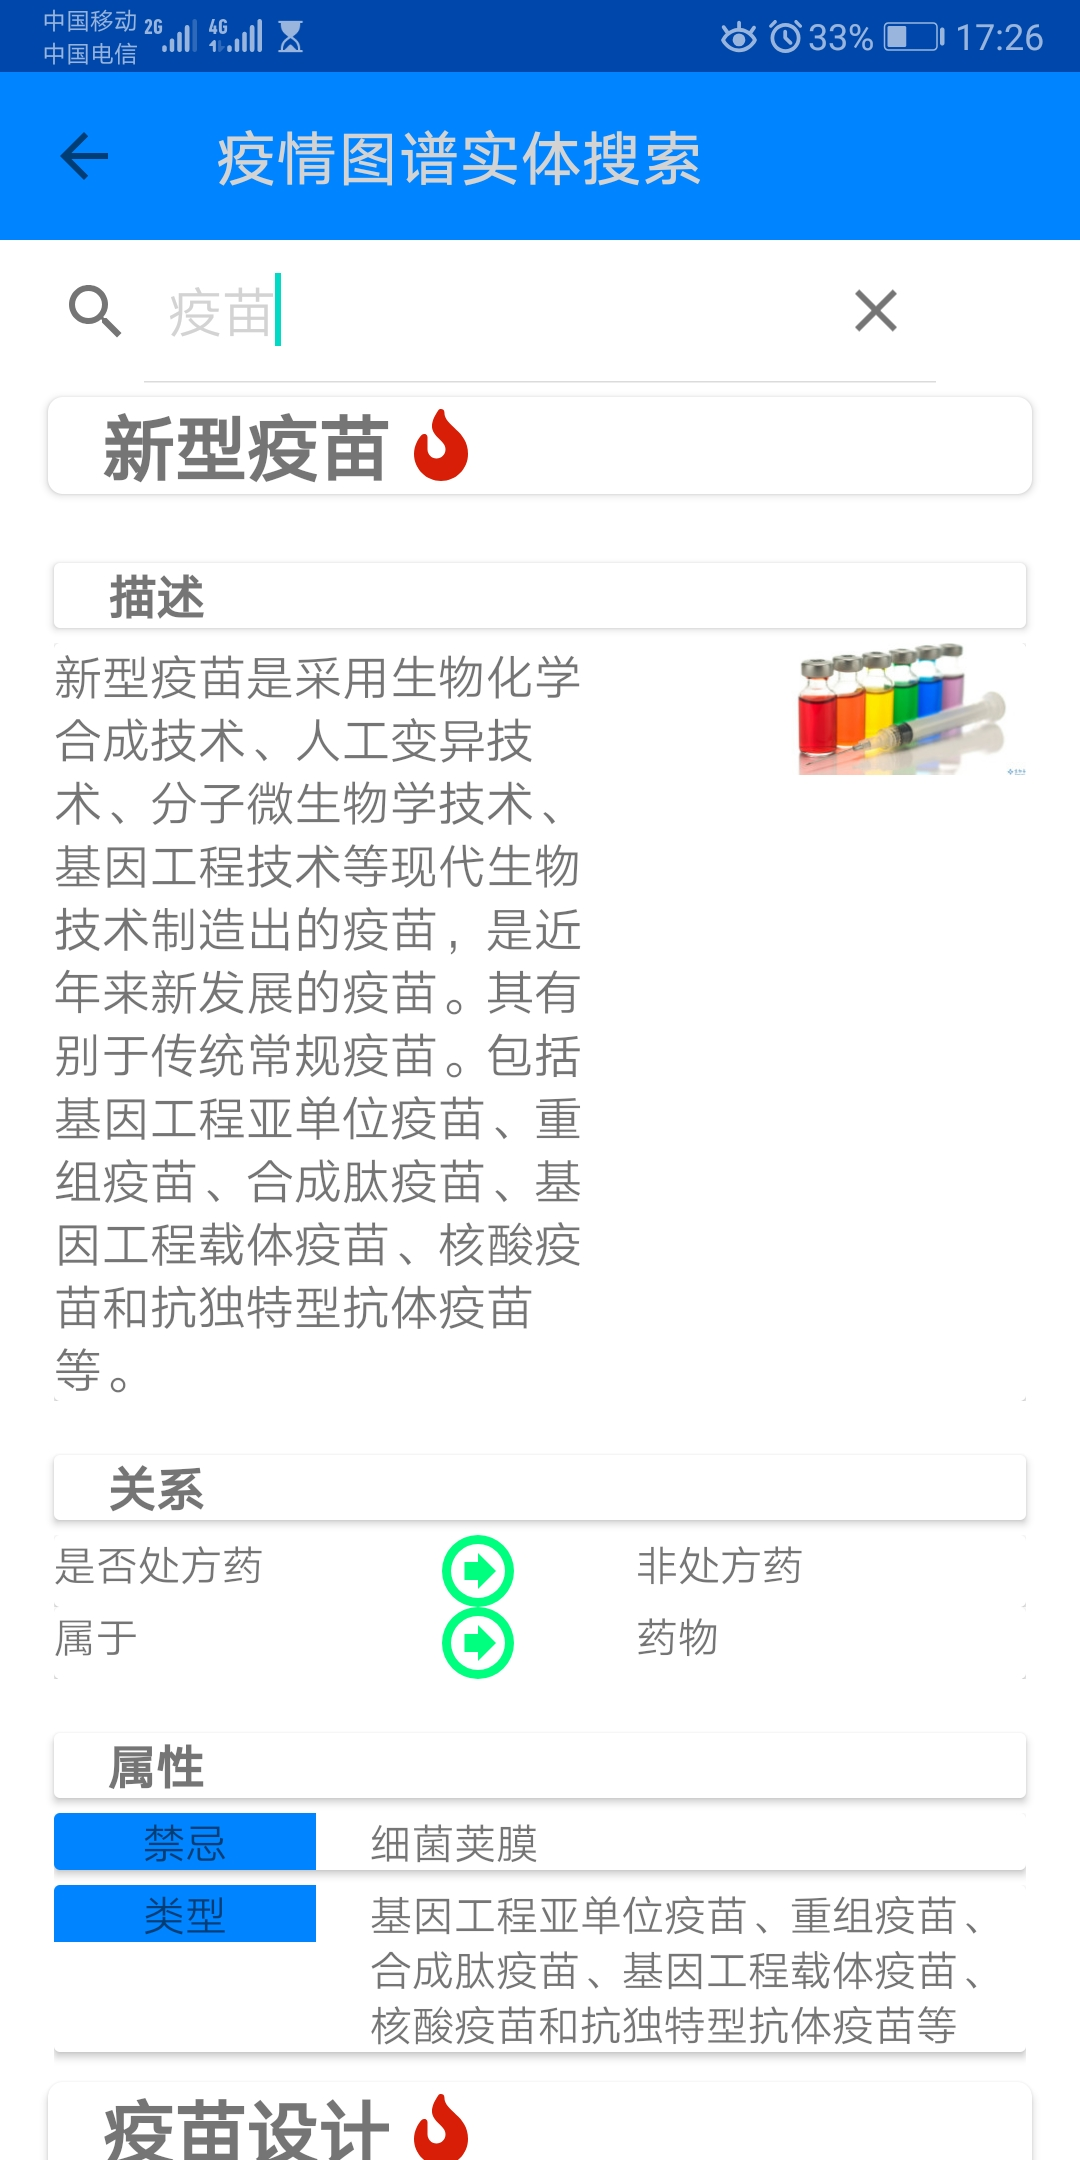
\includegraphics[width=5.5cm]{searchentity4}
%     }
%     \caption{实体搜索页面}
%     \end{figure}
            
\newpage
\subsubsection{新闻聚类}
新闻聚类页面合并到了主页面进行展示。主页面将聚类关键词展示到标签栏中,当切换到对应标签时显示对应关键词下聚类的结果。

\begin{figure}[htbp]
    \centering
    \subfigure[患者治疗类]{
        \begin{minipage}[t]{0.25\linewidth}
        \centering
        
\includegraphics[width=0.8\textwidth]{cluster2.jpg}
        %\caption{fig2}
        \end{minipage}%
        }%
    \subfigure[疫苗药物类]{
        \begin{minipage}[t]{0.25\linewidth}
        \centering
        
\includegraphics[width=0.8\textwidth]{cluster}
        %\caption{fig2}
        \end{minipage}%
        }%
    \subfigure[病毒研究类]{
    \begin{minipage}[t]{0.25\linewidth}
    \centering
    
\includegraphics[width=0.8\textwidth]{cluster3.jpg}
    %\caption{fig1}
    \end{minipage}%
    }%
    \subfigure[疫情形势类]{
    \begin{minipage}[t]{0.25\linewidth}
    \centering
    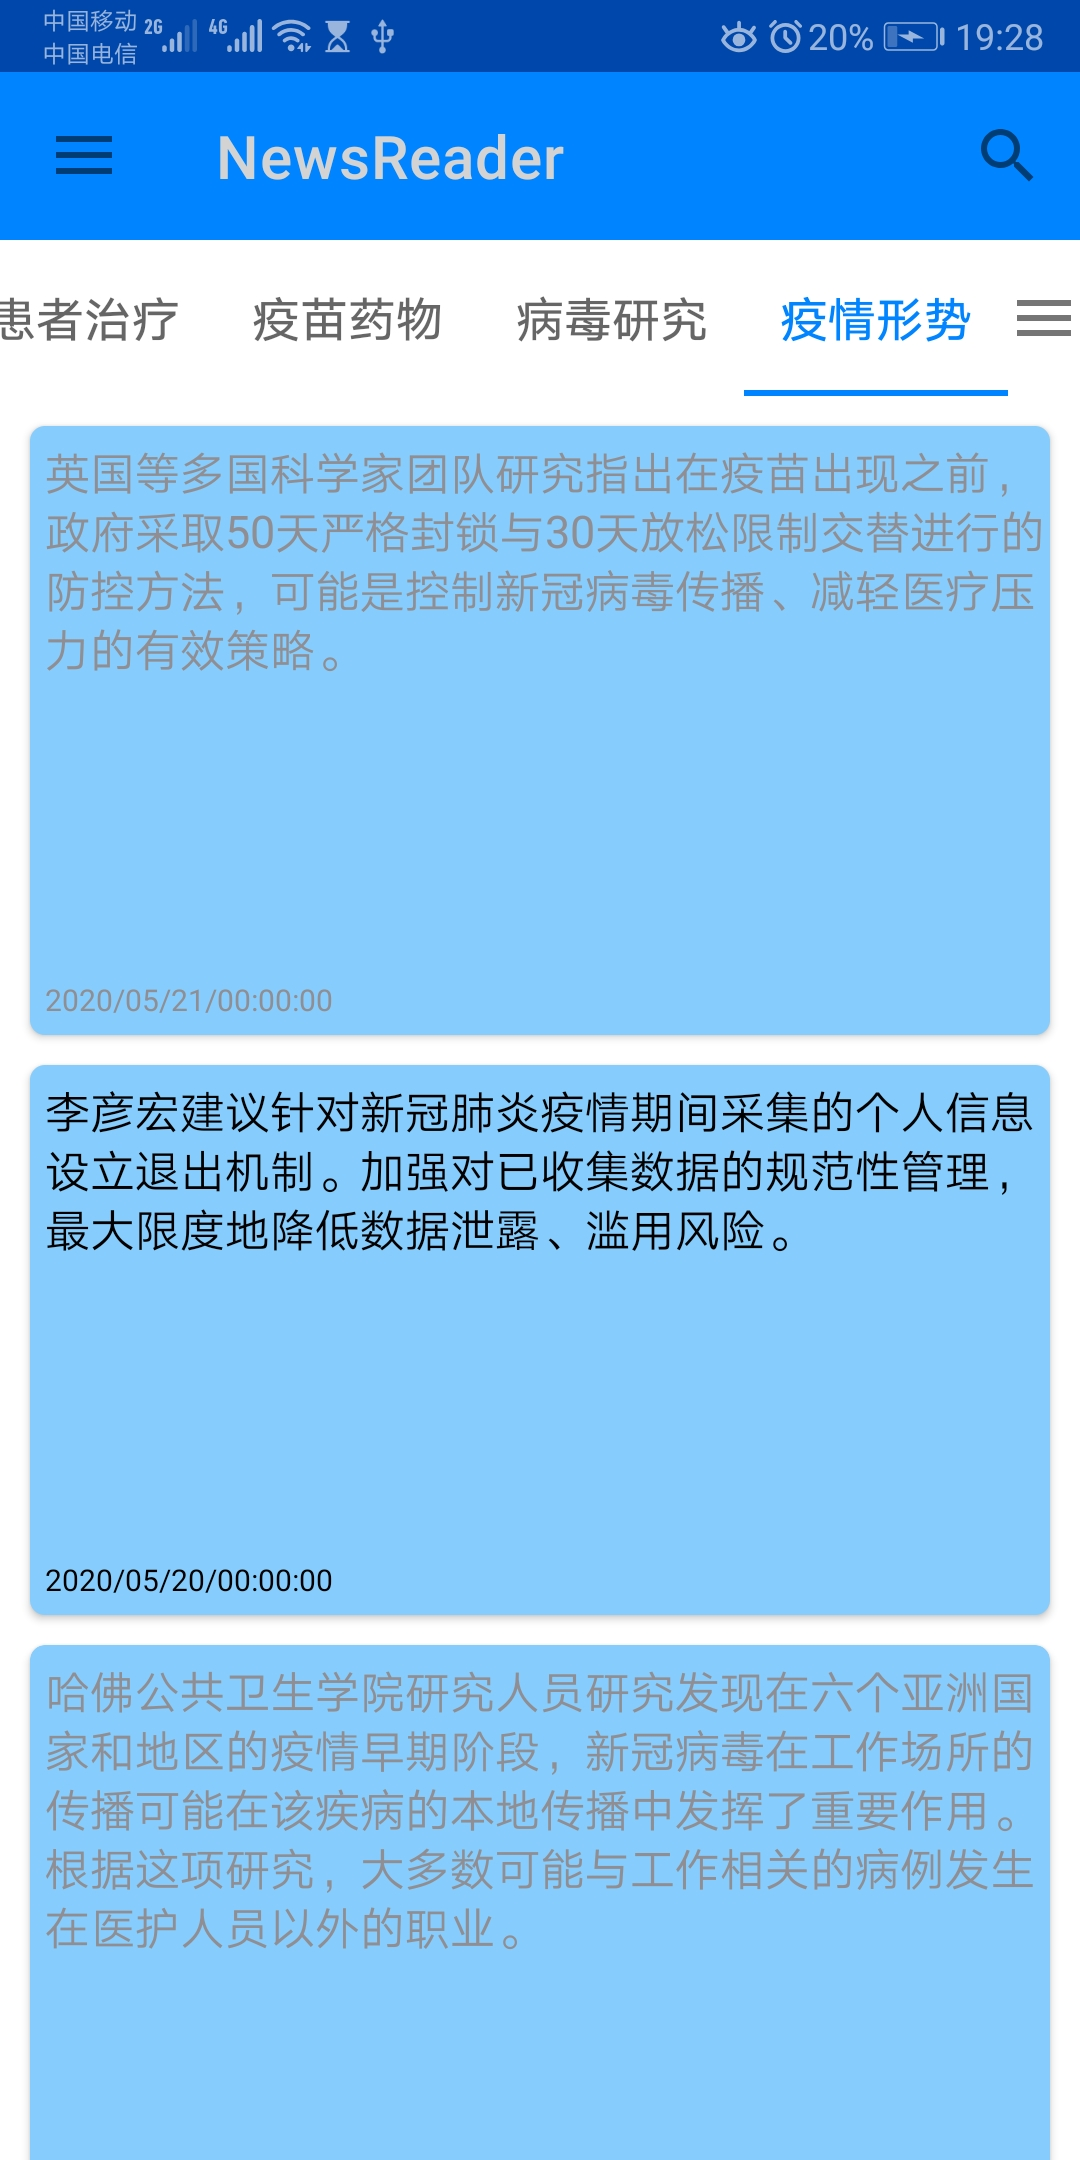
\includegraphics[width=0.8\textwidth]{cluster4}
    %\caption{fig2}
    \end{minipage}%
    }%

    \centering
    \caption{聚类展示页面}
    \end{figure}

% \begin{figure}[h]
%     \label{Ratio}
%     \centering
%         
\includegraphics[height=0.5\textwidth]{cluster}
%         \caption{聚类展示页面}
%     \end{figure}

\subsubsection{知疫学者展示}
知疫学者页面的实现逻辑和新闻列表页面类似。同样是通过RecyclerView实现了学者列表的展示、点击进入对应的学者详情页。
学者详情页展示了学者的姓名、照片、职位、简介、教育经历、工作经历等。

\begin{figure}[htbp]
    \centering
    \subfigure[高关注学者]{
        \begin{minipage}[t]{0.25\linewidth}
        \centering
        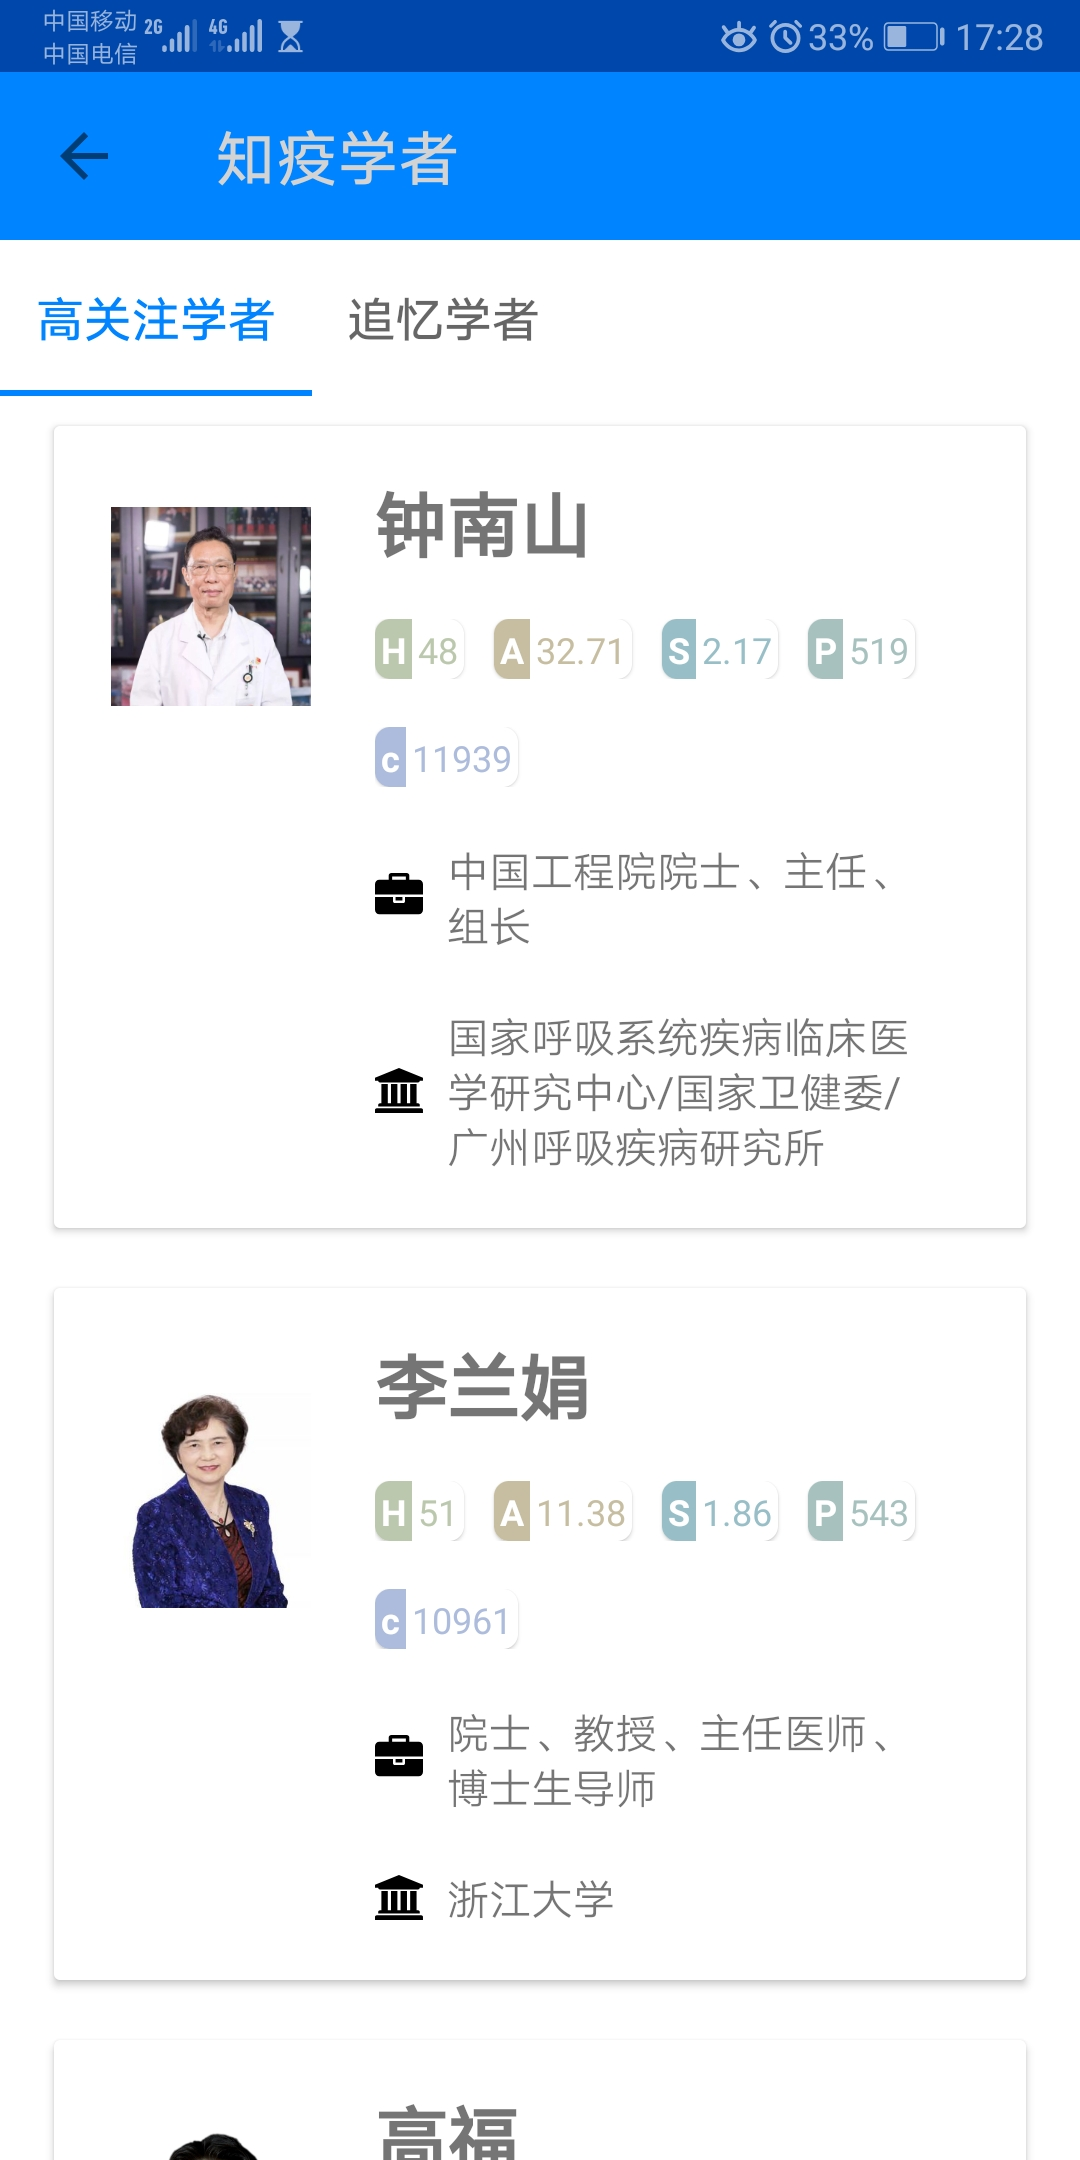
\includegraphics[width=0.8\textwidth]{scholar1}
        %\caption{fig2}
        \end{minipage}%
        }%
    \subfigure[追忆学者]{
        \begin{minipage}[t]{0.25\linewidth}
        \centering
        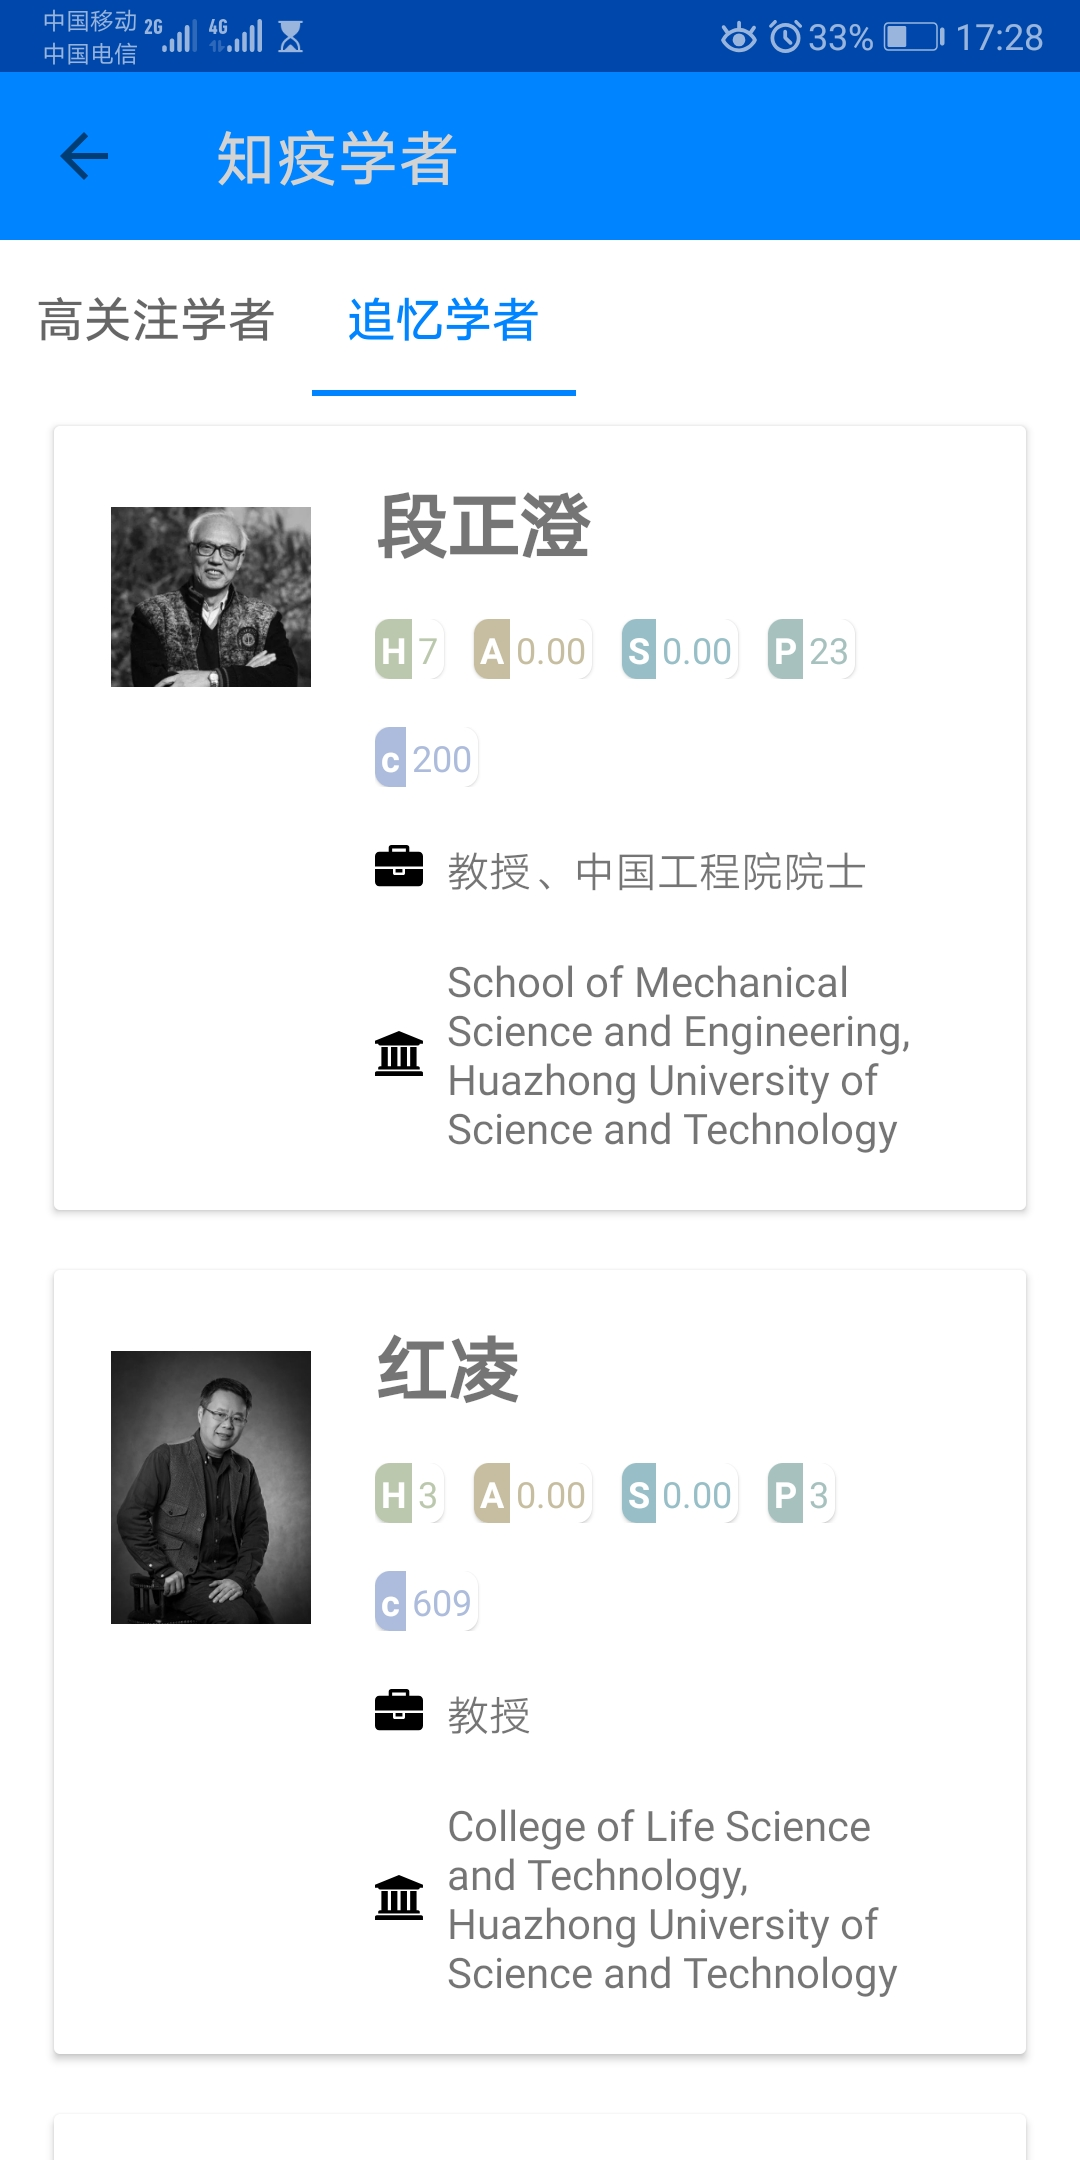
\includegraphics[width=0.8\textwidth]{scholar2}
        %\caption{fig2}
        \end{minipage}%
        }%
    \subfigure[高关注学者详情页]{
    \begin{minipage}[t]{0.25\linewidth}
    \centering
    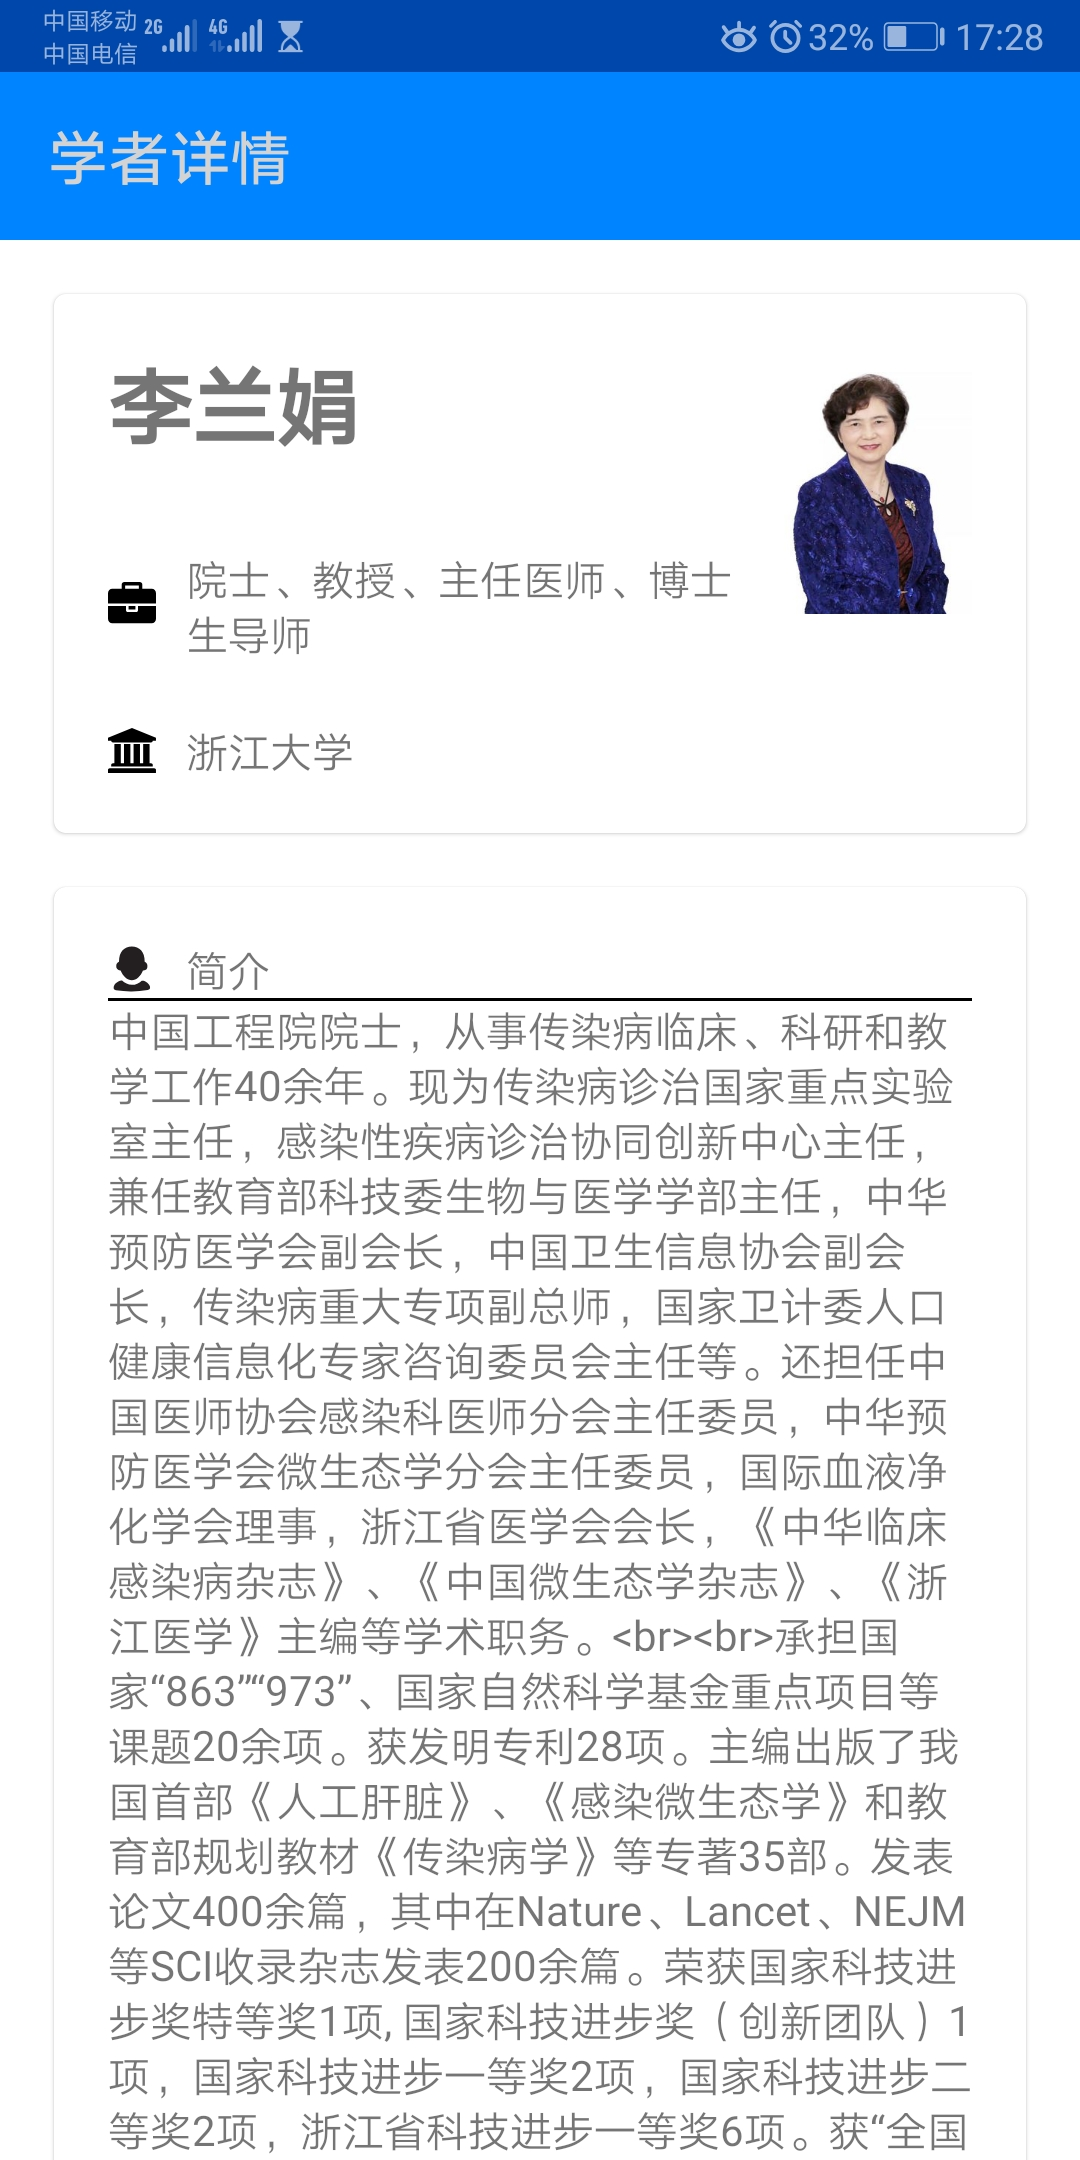
\includegraphics[width=0.8\textwidth]{scholar3}
    %\caption{fig1}
    \end{minipage}%
    }%
    \subfigure[追忆学者详情页]{
    \begin{minipage}[t]{0.25\linewidth}
    \centering
    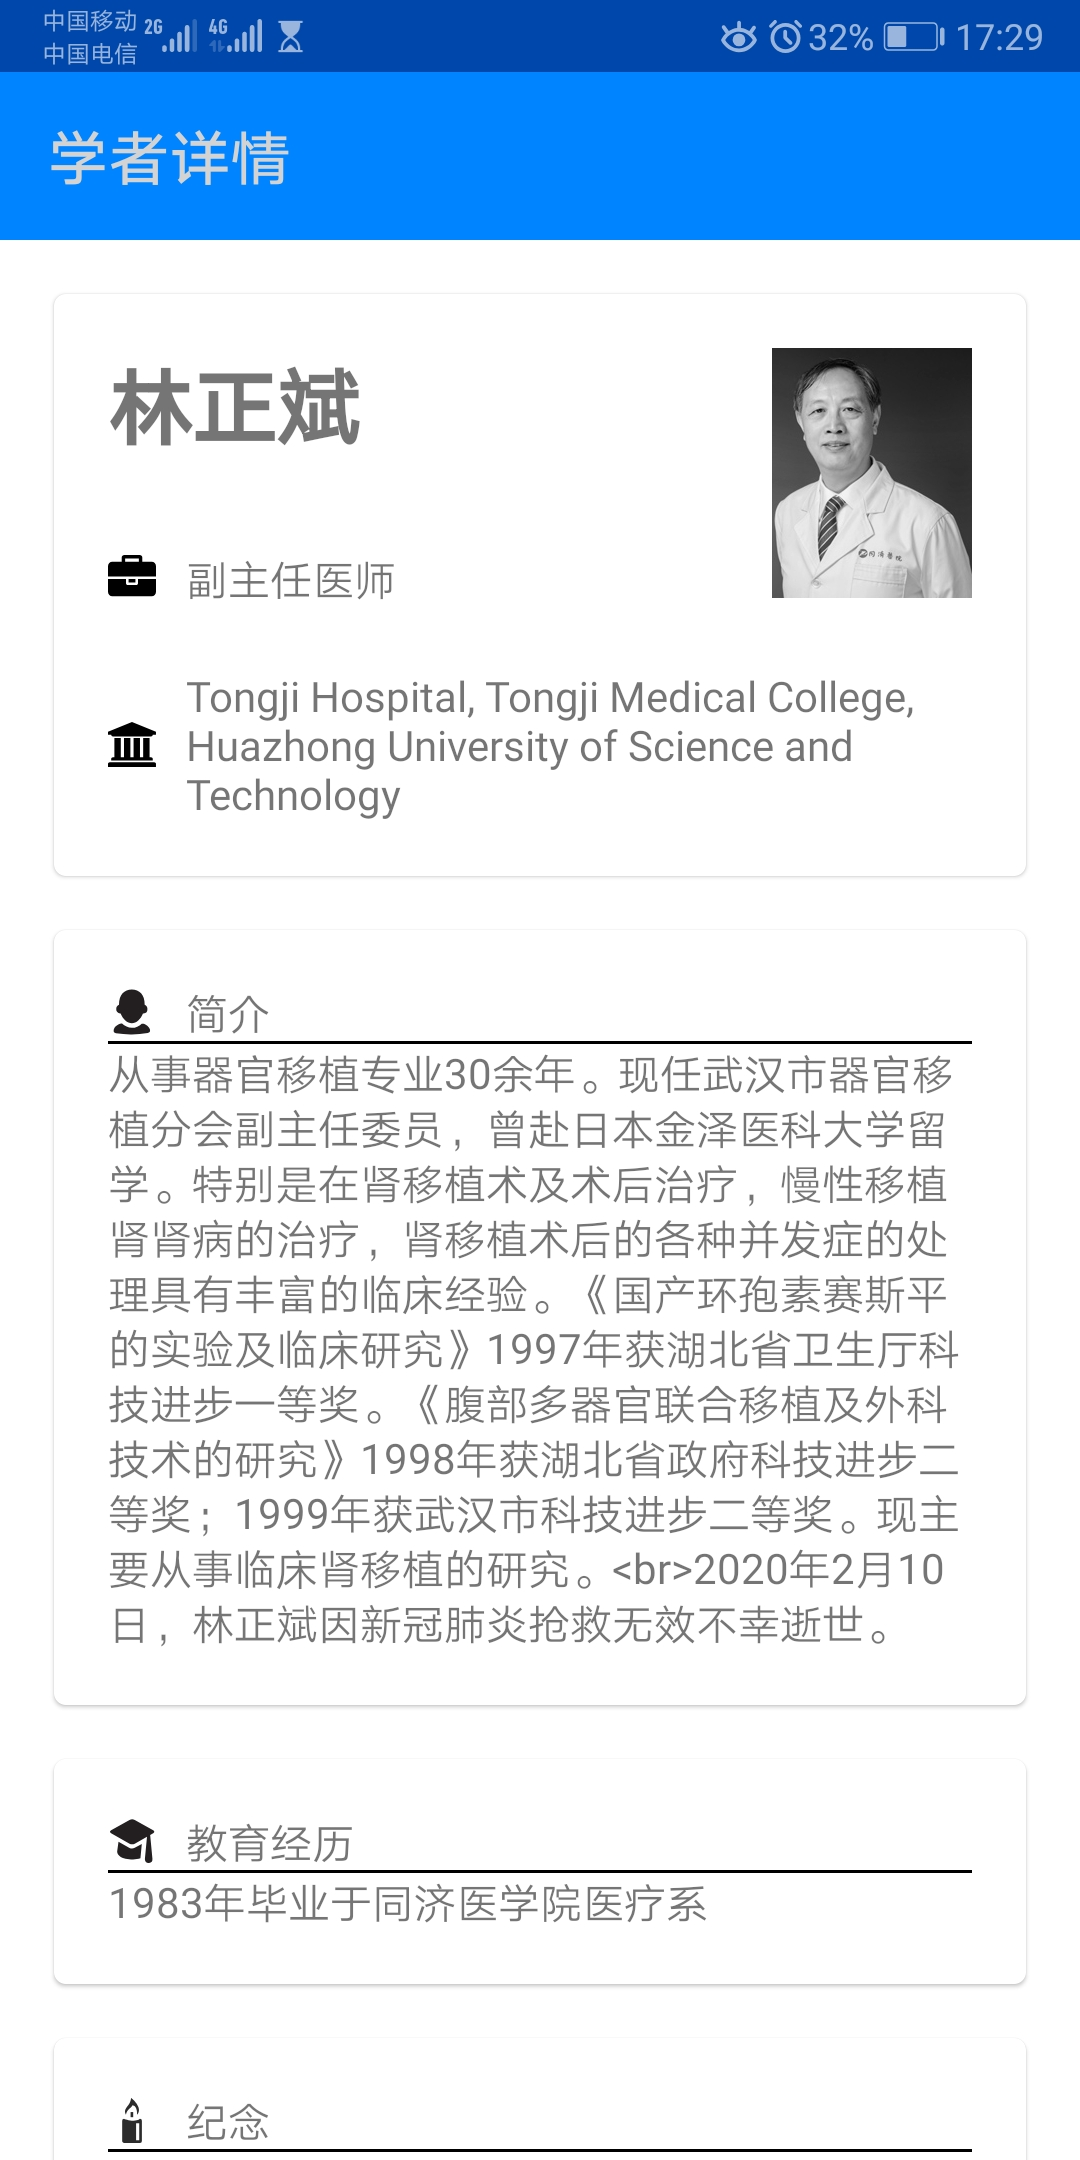
\includegraphics[width=0.8\textwidth]{scholar4}
    %\caption{fig2}
    \end{minipage}%
    }%

    \centering
    \caption{知疫学者页面}
    \end{figure}

% \begin{figure}[h]
%     \centering
%     \subfigure[高关注学者]{
%     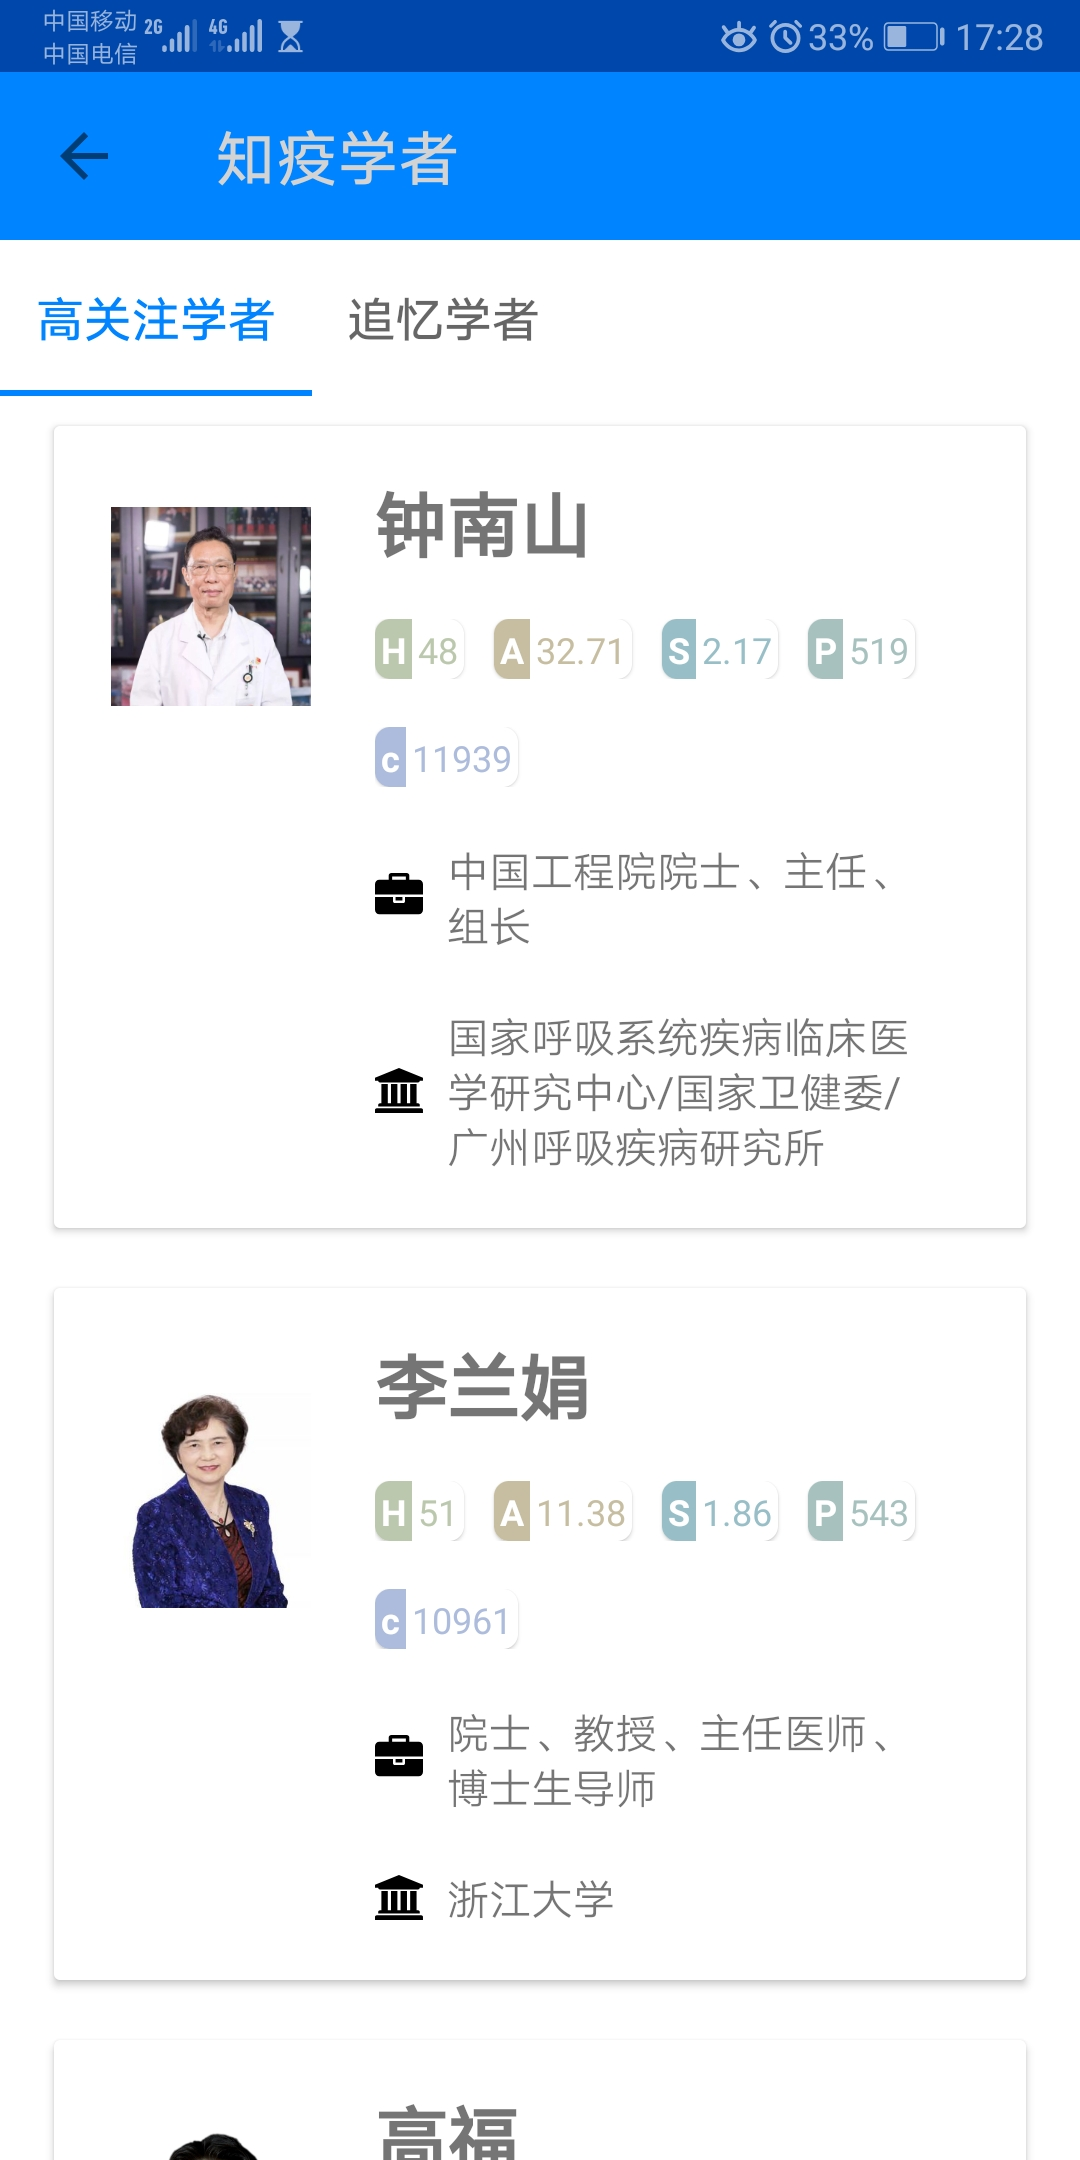
\includegraphics[width=5.5cm]{scholar1}
%     }
%     \quad
%     \subfigure[追忆学者]{
%     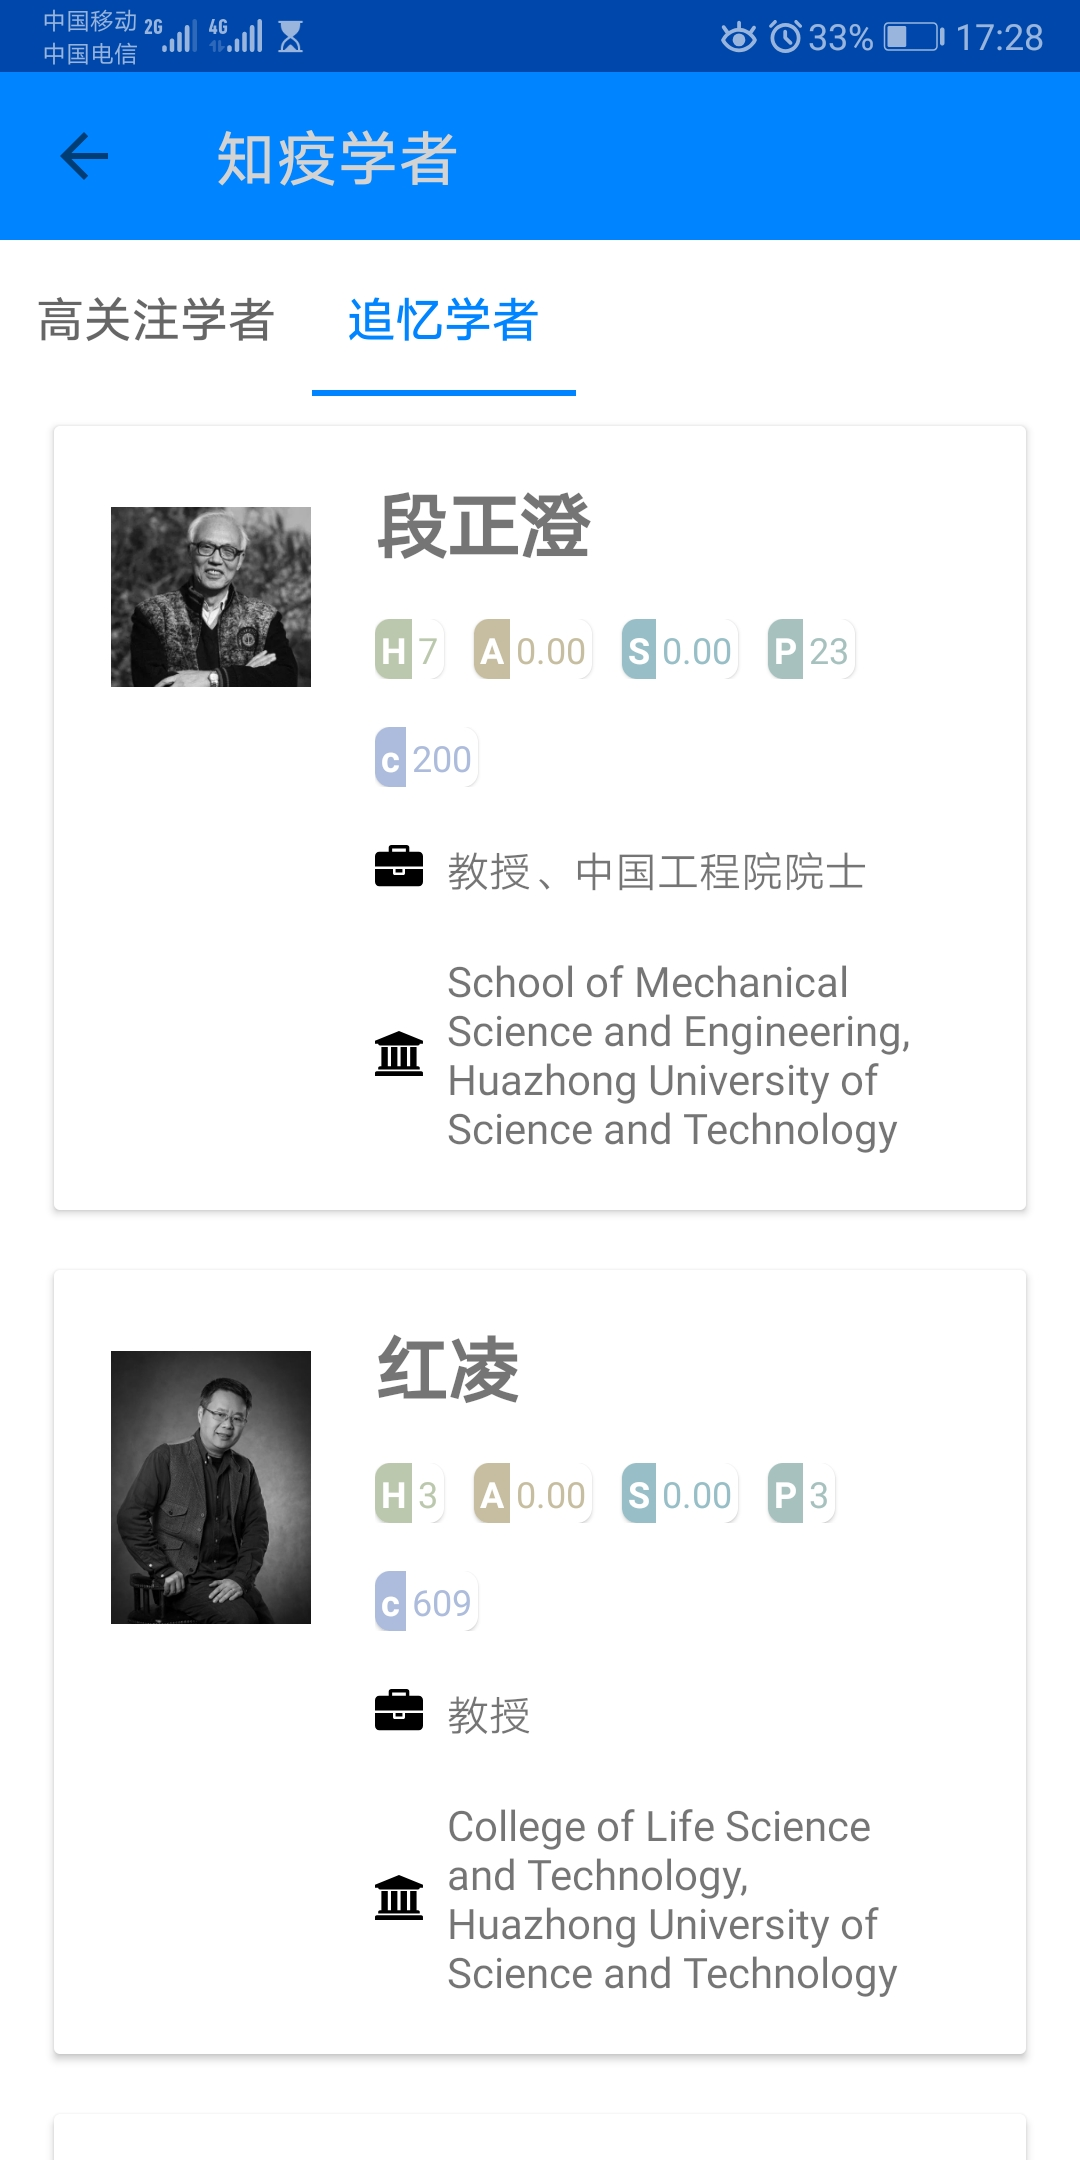
\includegraphics[width=5.5cm]{scholar2}
%     }
%     \quad
%     \subfigure[高关注学者详情页]{
%     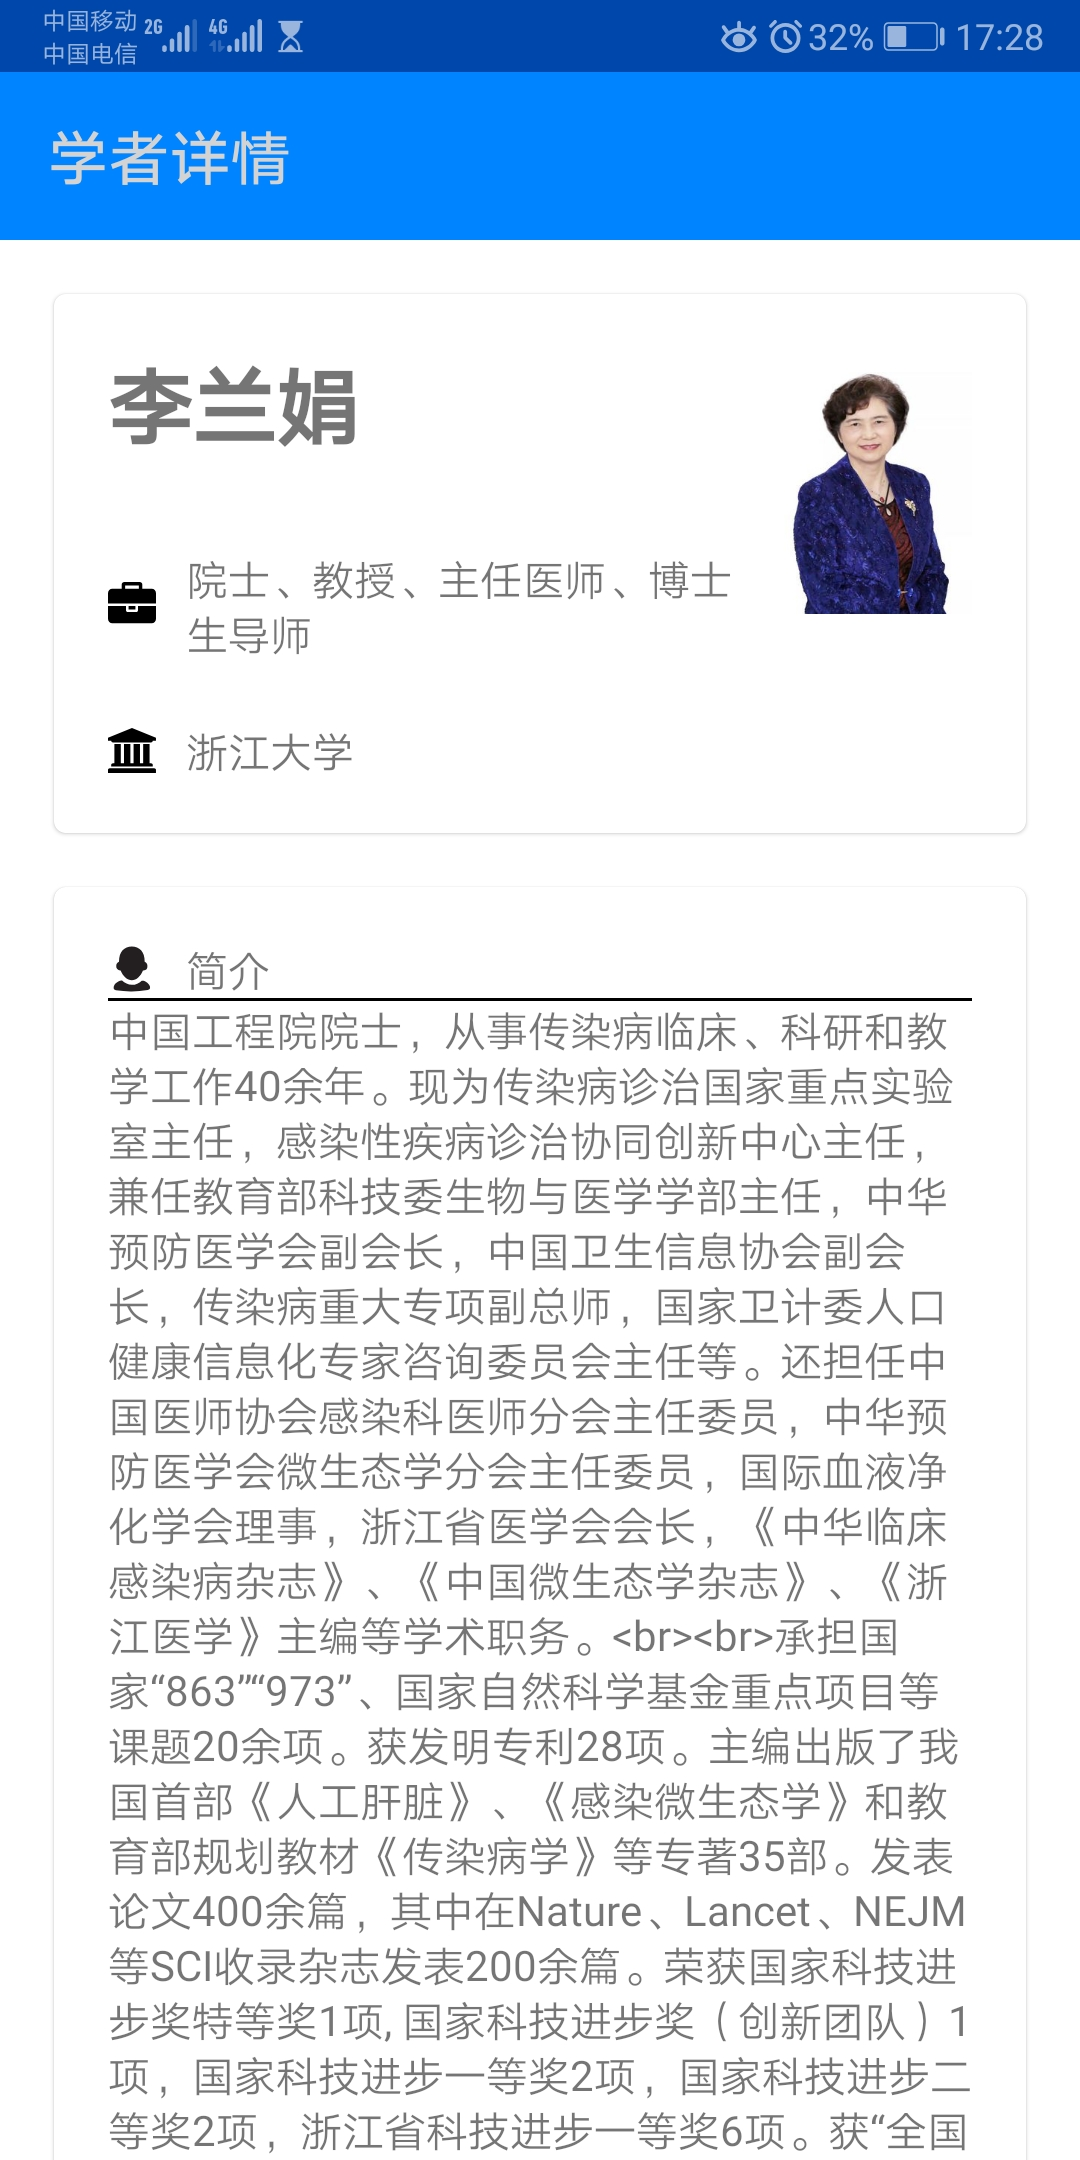
\includegraphics[width=5.5cm]{scholar3}
%     }
%     \quad
%     \subfigure[追忆学者详情页]{
%     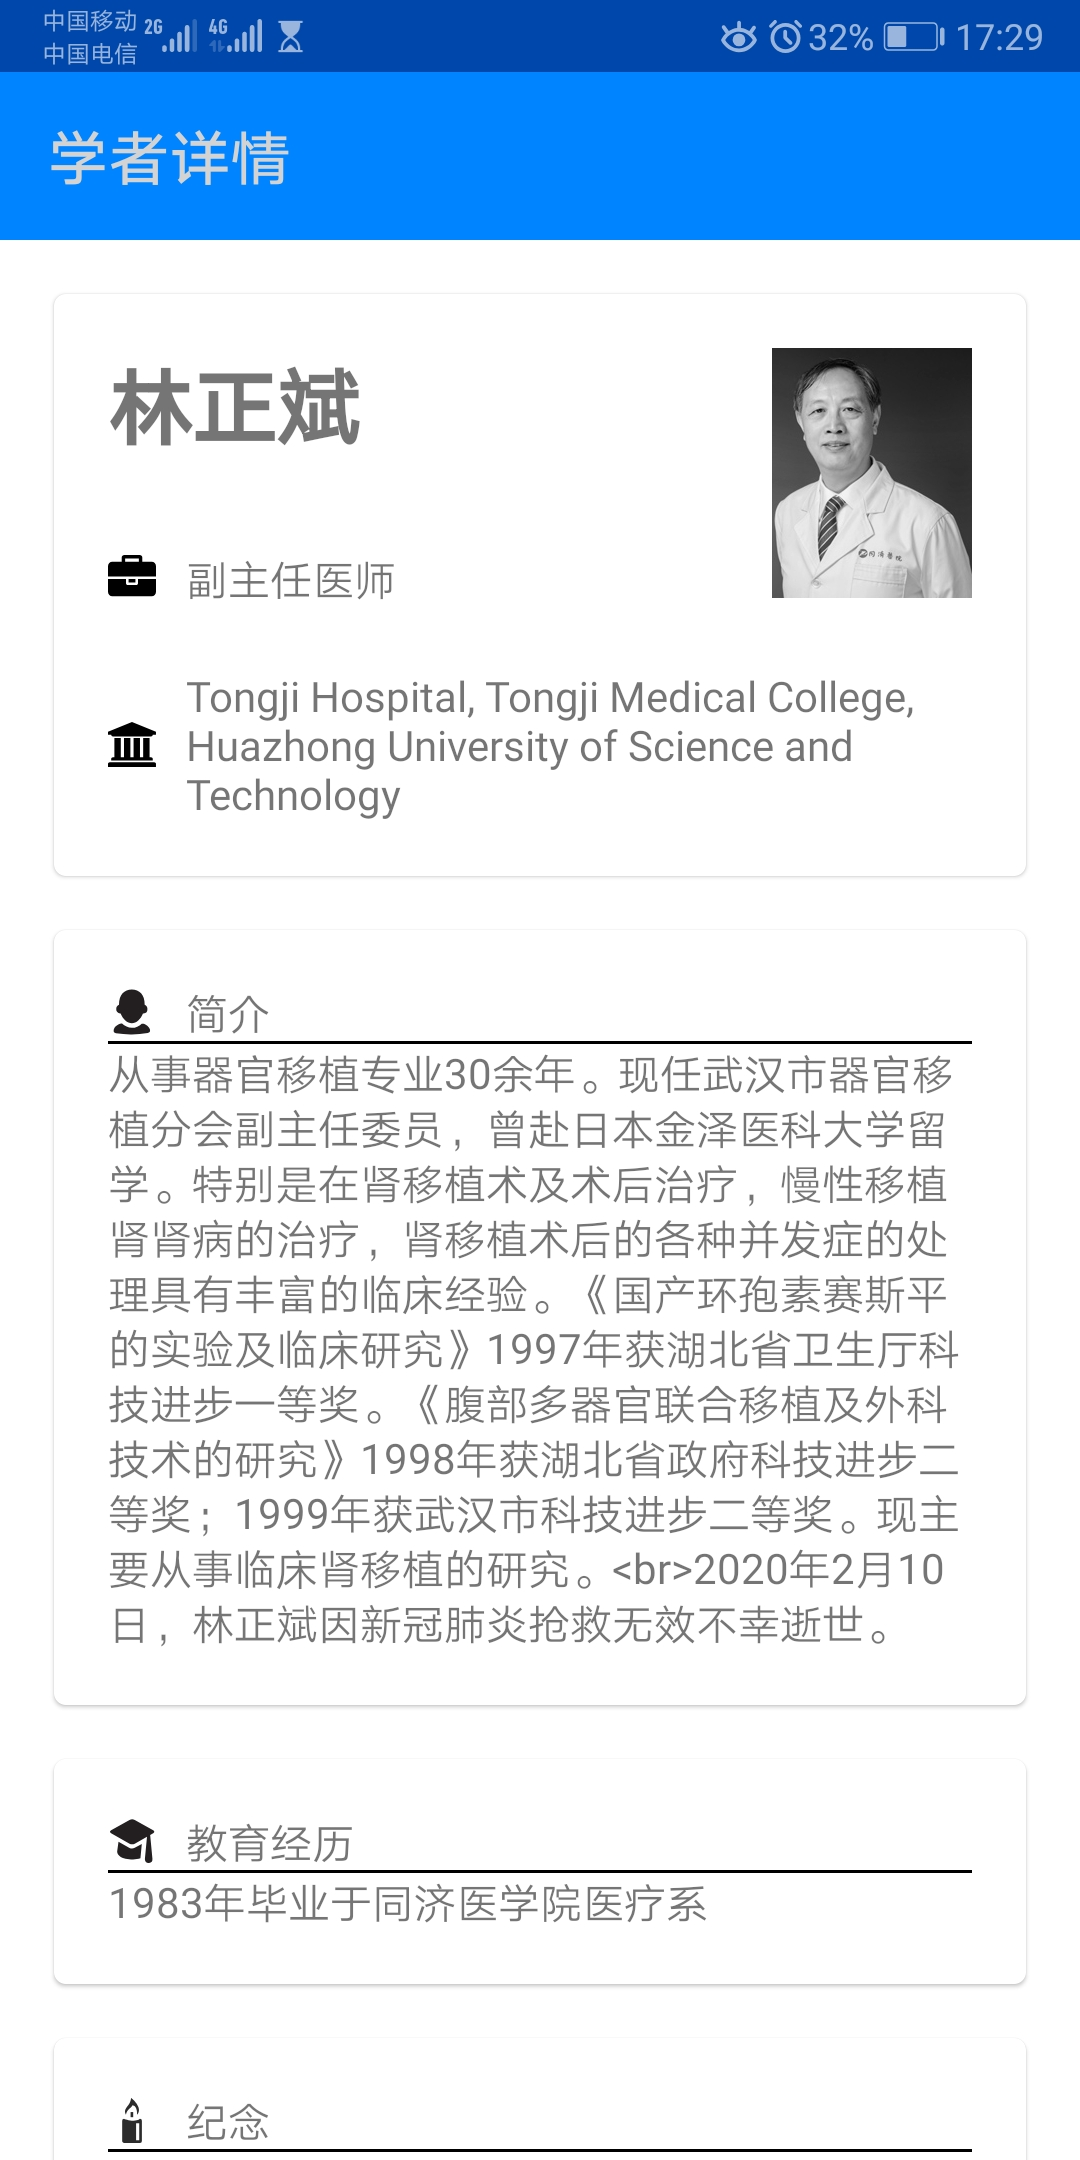
\includegraphics[width=5.5cm]{scholar4}
%     }
%     \caption{知疫学者页面}
%     \end{figure}


\subsubsection{夜间模式}
夜间模式并非本次作业的硬性要求,我在这里进行了一些简单的学习和尝试。对于非官方控件需要自行配置values文件夹下的color(night)文件,才能够实现夜间模式时的颜色变化。

通过AppCompatDelegate.setDefaultNightMode函数可以实现基础的夜间模式(会自动对不同色彩进行匹配)。
\begin{figure}[htbp]
    \centering
    \subfigure[夜间模式下侧边栏]{
        \begin{minipage}[t]{0.25\linewidth}
        \centering
        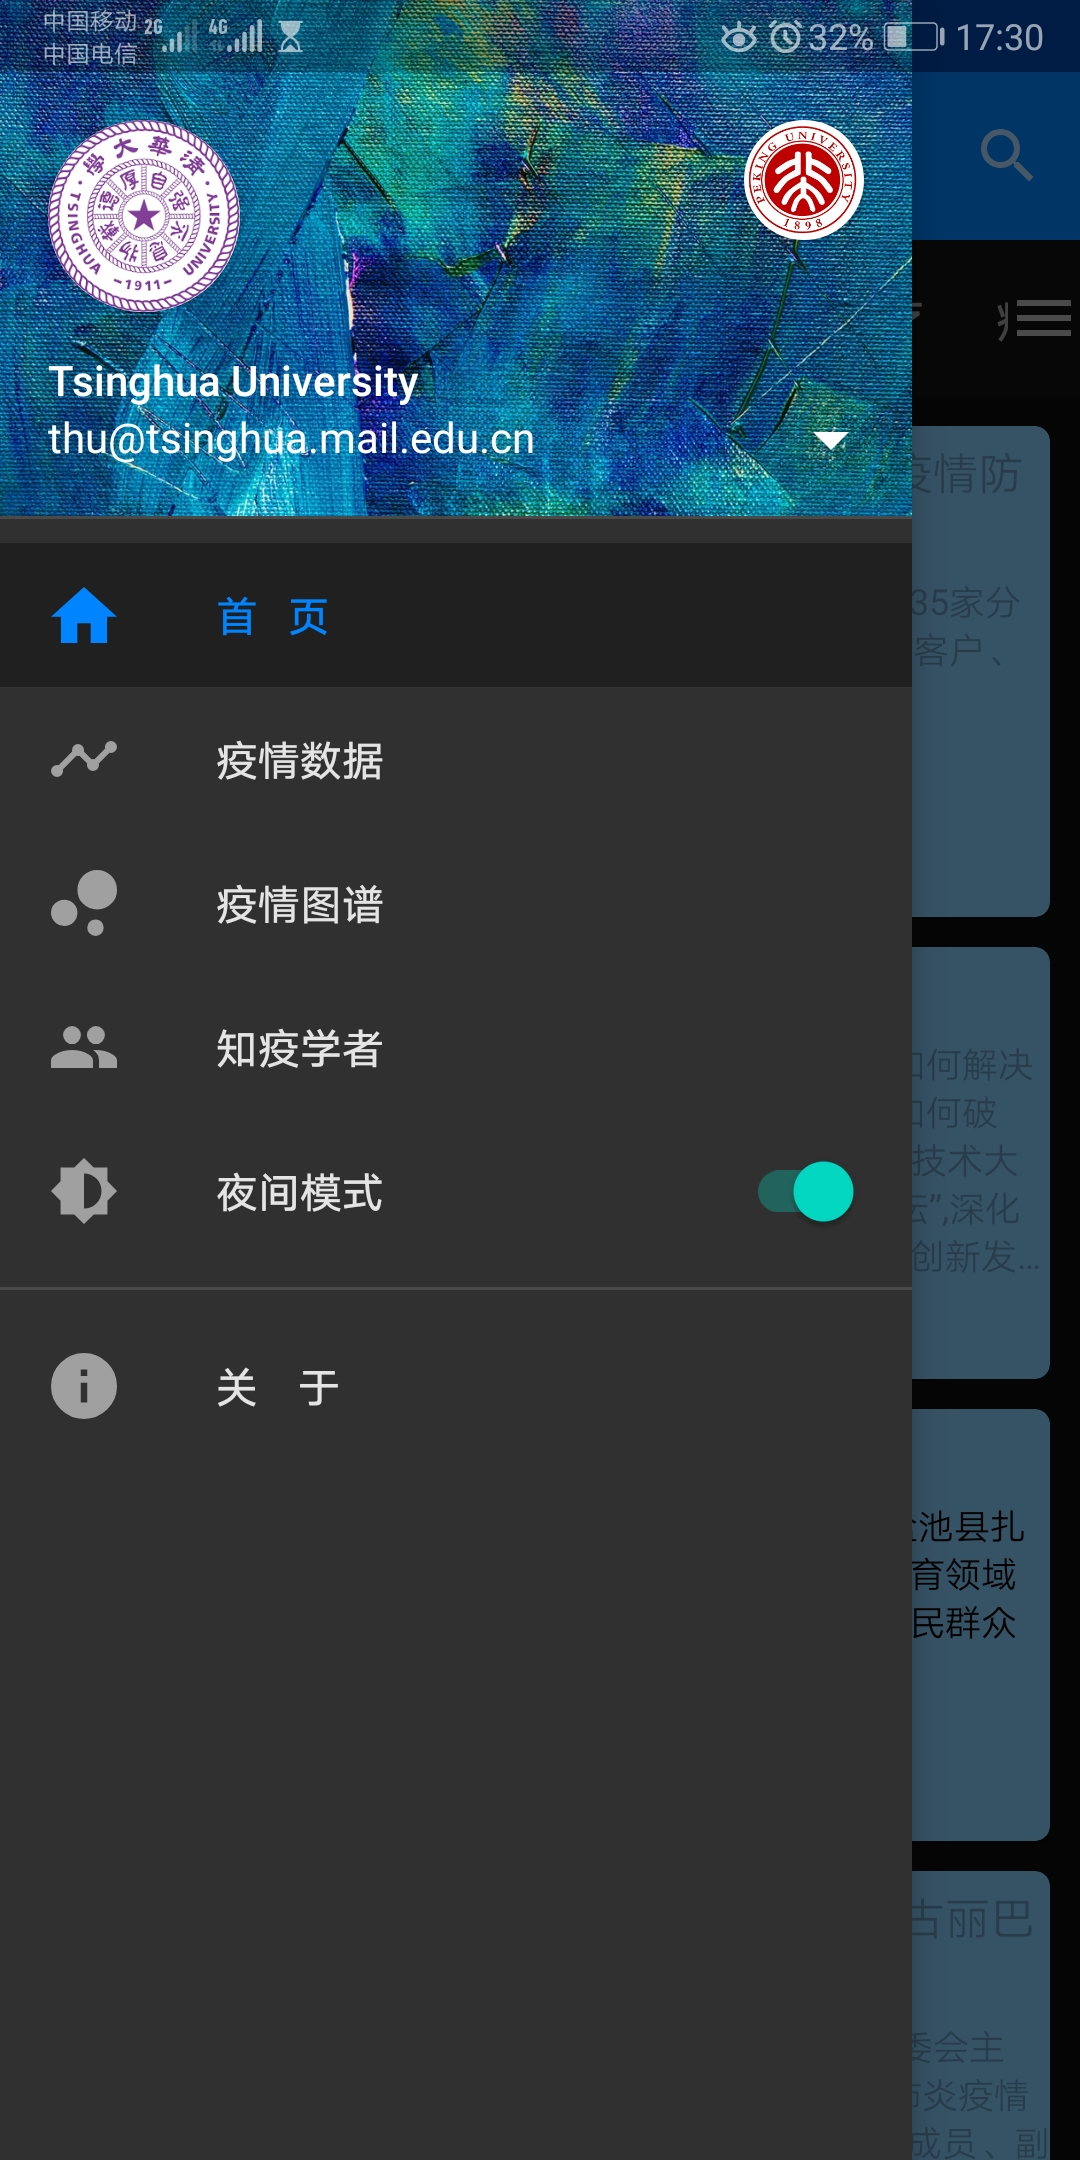
\includegraphics[width=0.8\textwidth]{nightmode1}
        %\caption{fig2}
        \end{minipage}%
        }%
    \subfigure[夜间模式下新闻列表]{
        \begin{minipage}[t]{0.25\linewidth}
        \centering
        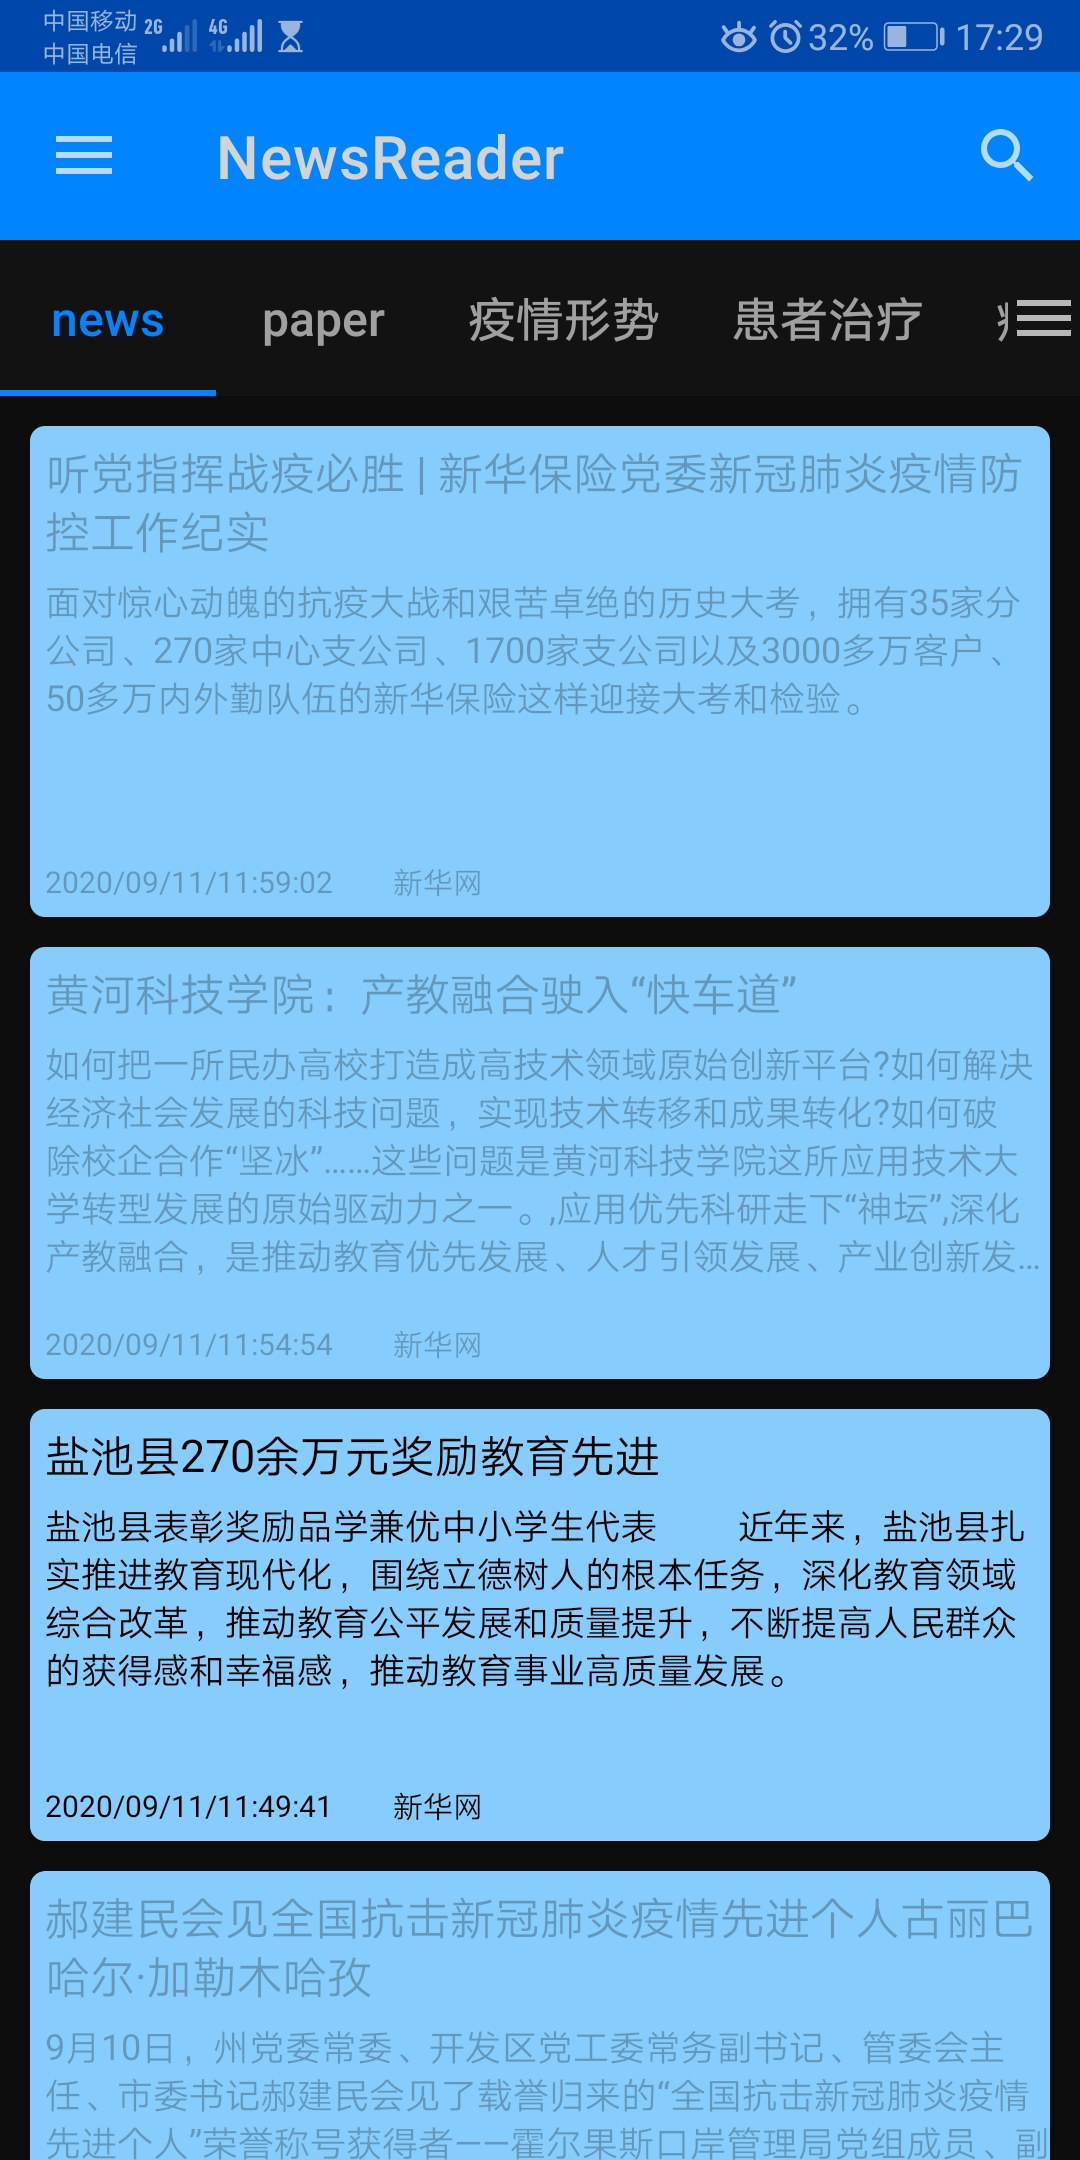
\includegraphics[width=0.8\textwidth]{nightmode2}
        %\caption{fig2}
        \end{minipage}%
        }%
    \subfigure[夜间模式下实体搜索]{
    \begin{minipage}[t]{0.25\linewidth}
    \centering
    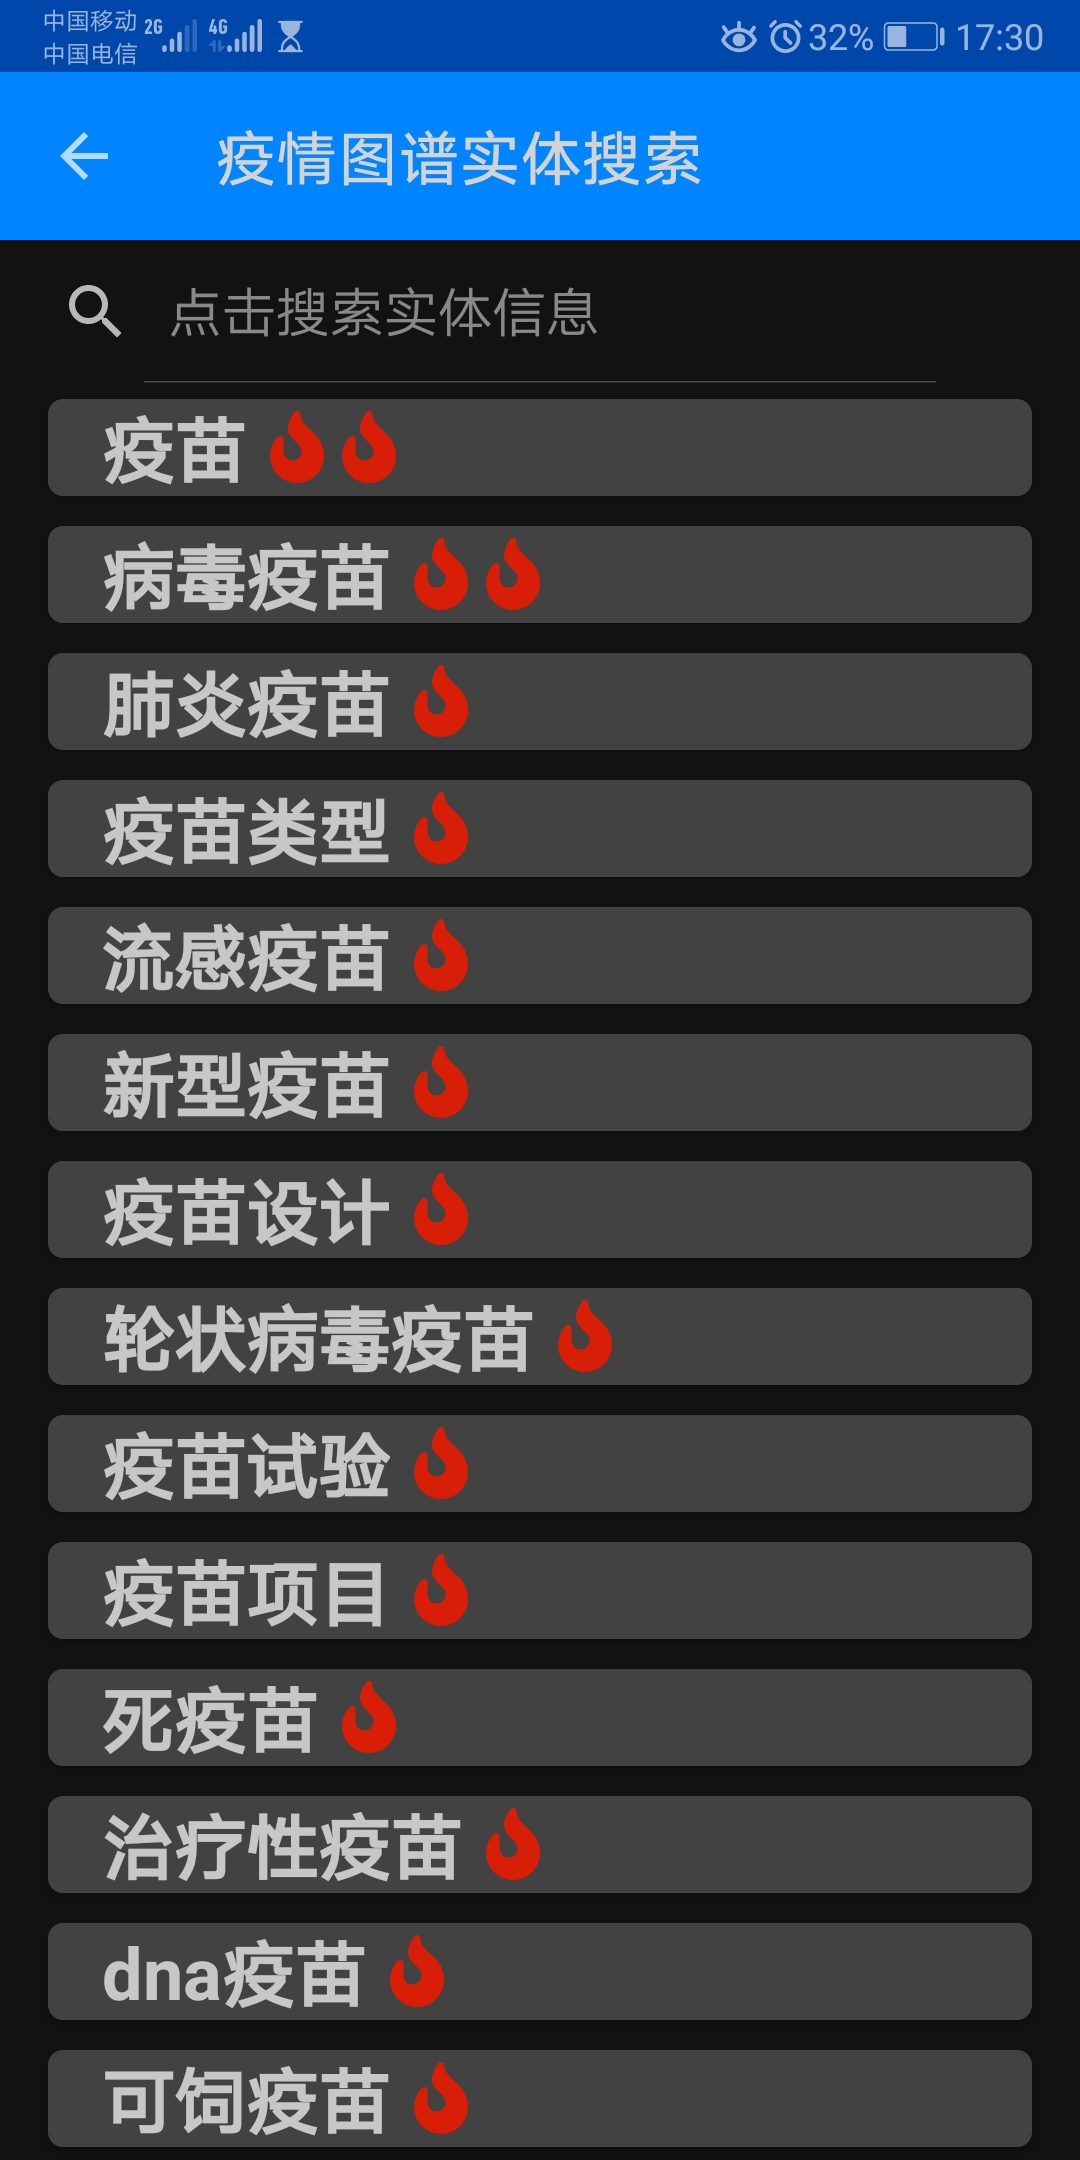
\includegraphics[width=0.8\textwidth]{nightmode3}
    %\caption{fig1}
    \end{minipage}%
    }%
    \subfigure[夜间模式下知疫学者]{
    \begin{minipage}[t]{0.25\linewidth}
    \centering
    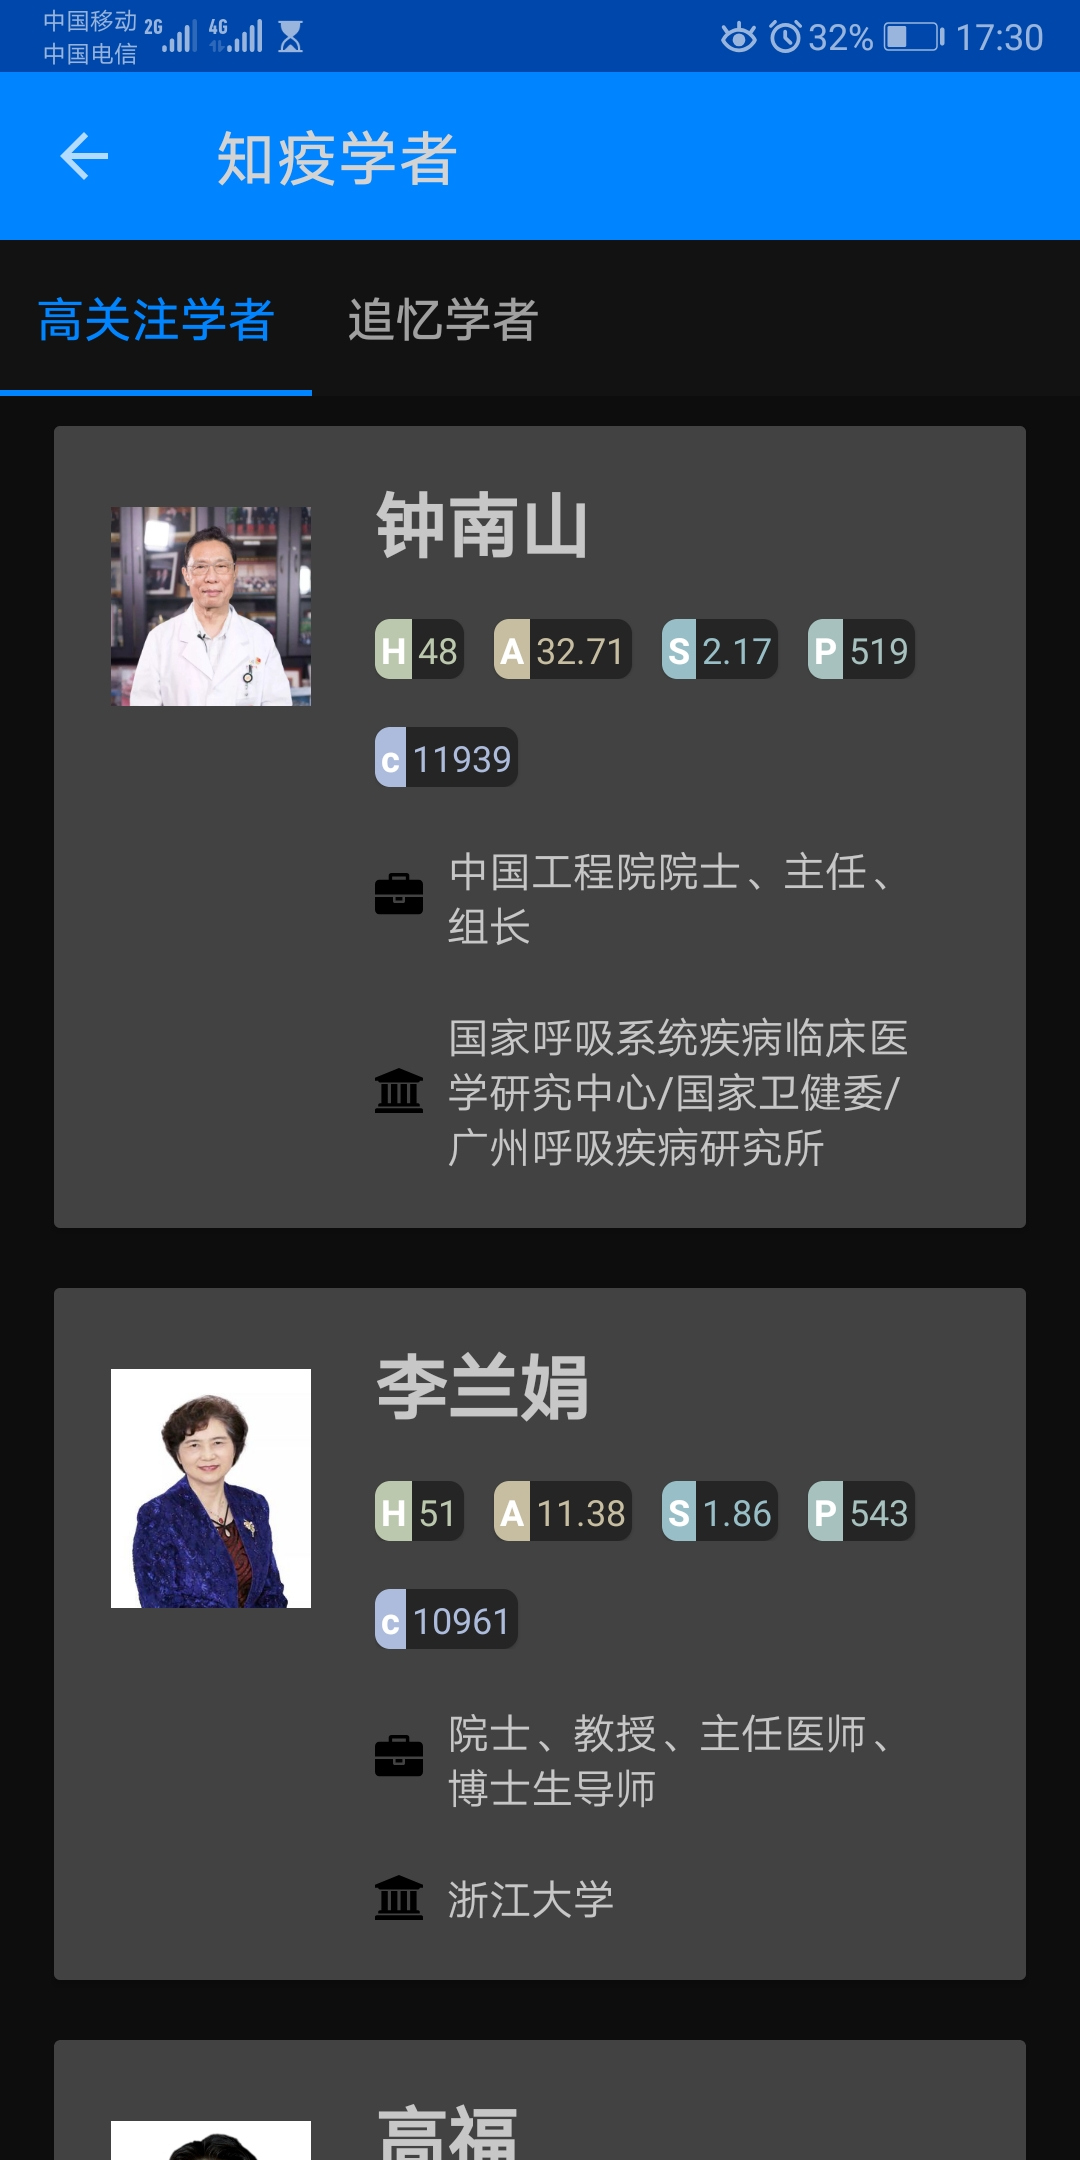
\includegraphics[width=0.8\textwidth]{nightmode4}
    %\caption{fig2}
    \end{minipage}%
    }%

    \centering
    \caption{夜间模式}
    \end{figure}

% \begin{figure}[h]
%     \centering
%     \subfigure[夜间模式下侧边栏]{
%     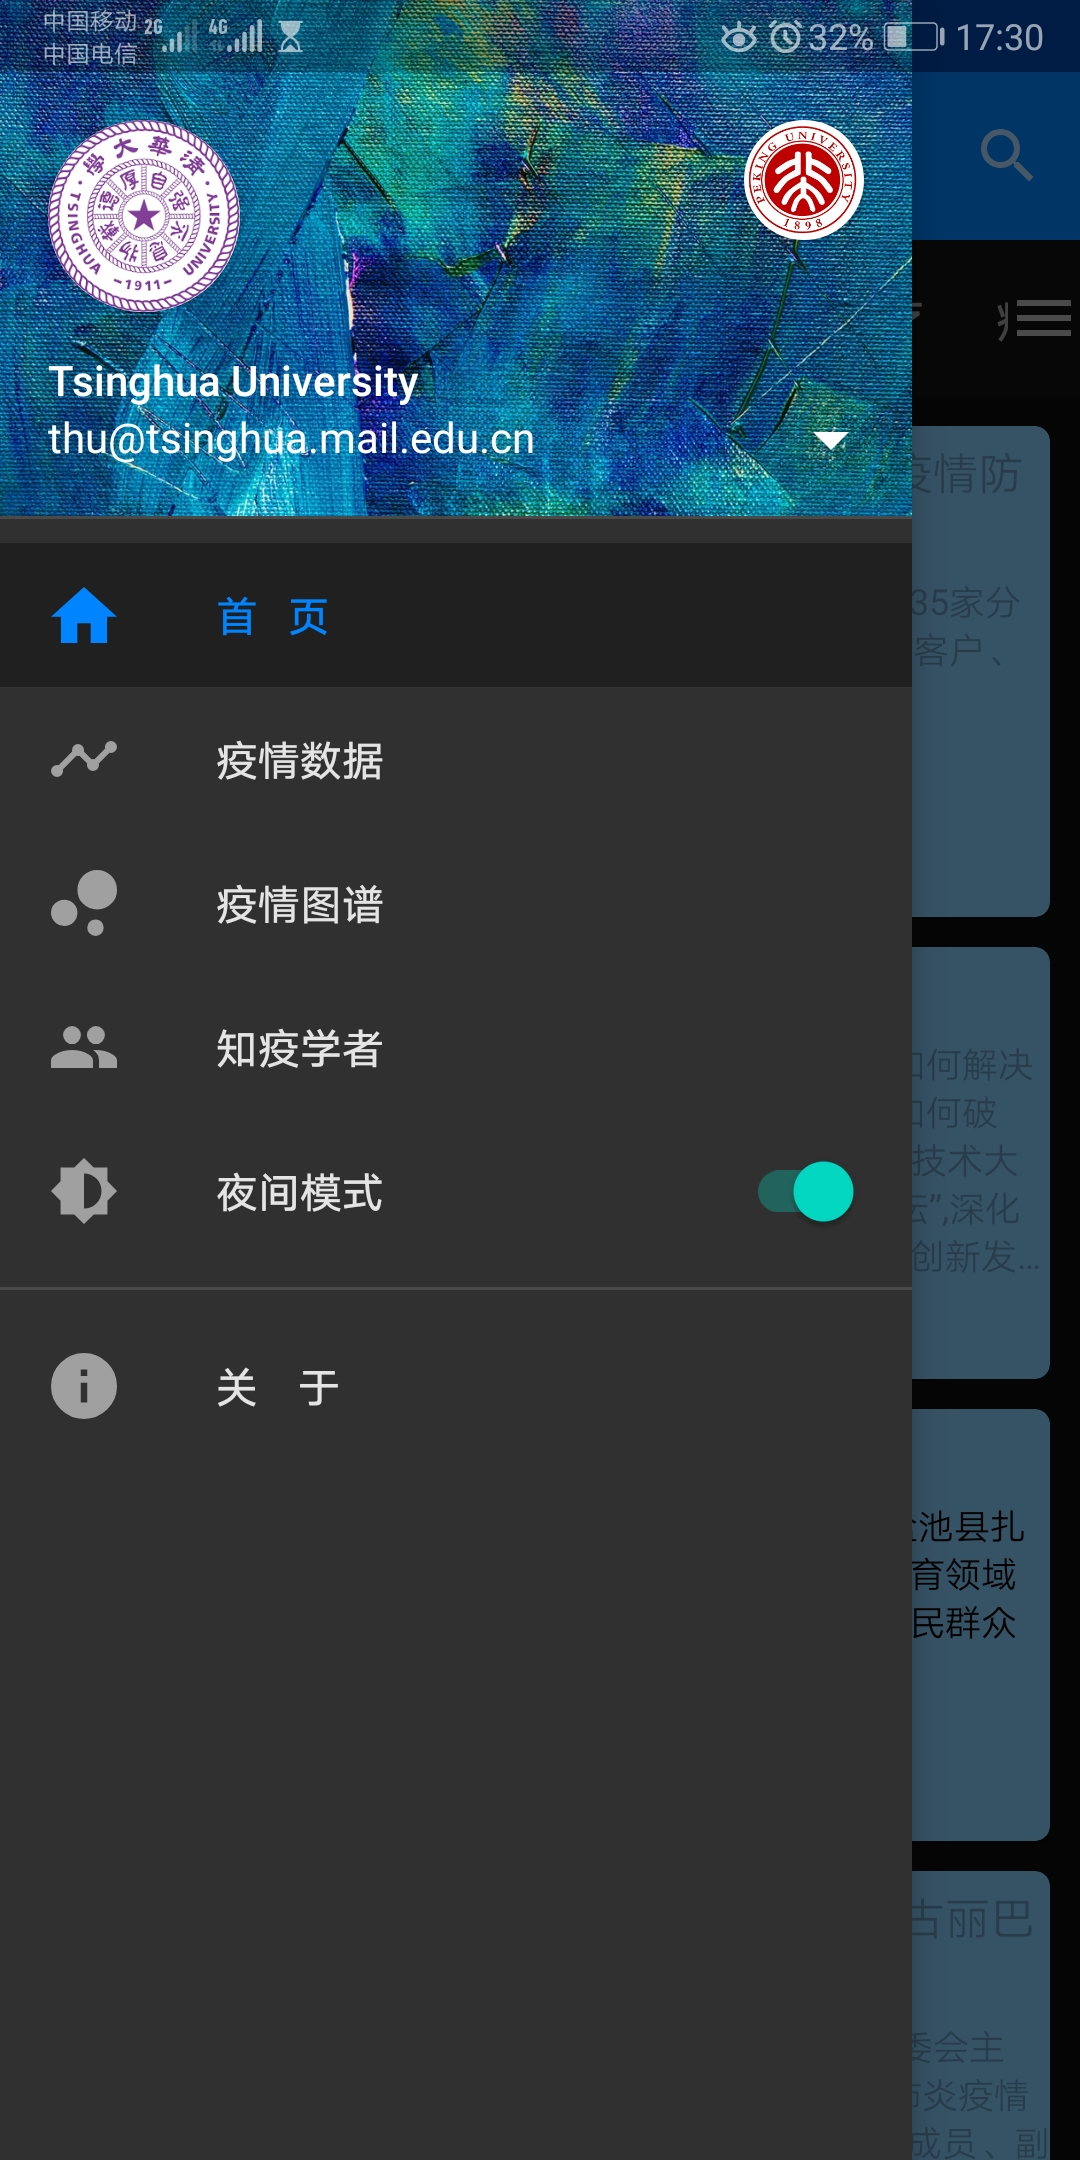
\includegraphics[width=5.5cm]{nightmode1}
%     }
%     \quad
%     \subfigure[夜间模式下新闻列表]{
%     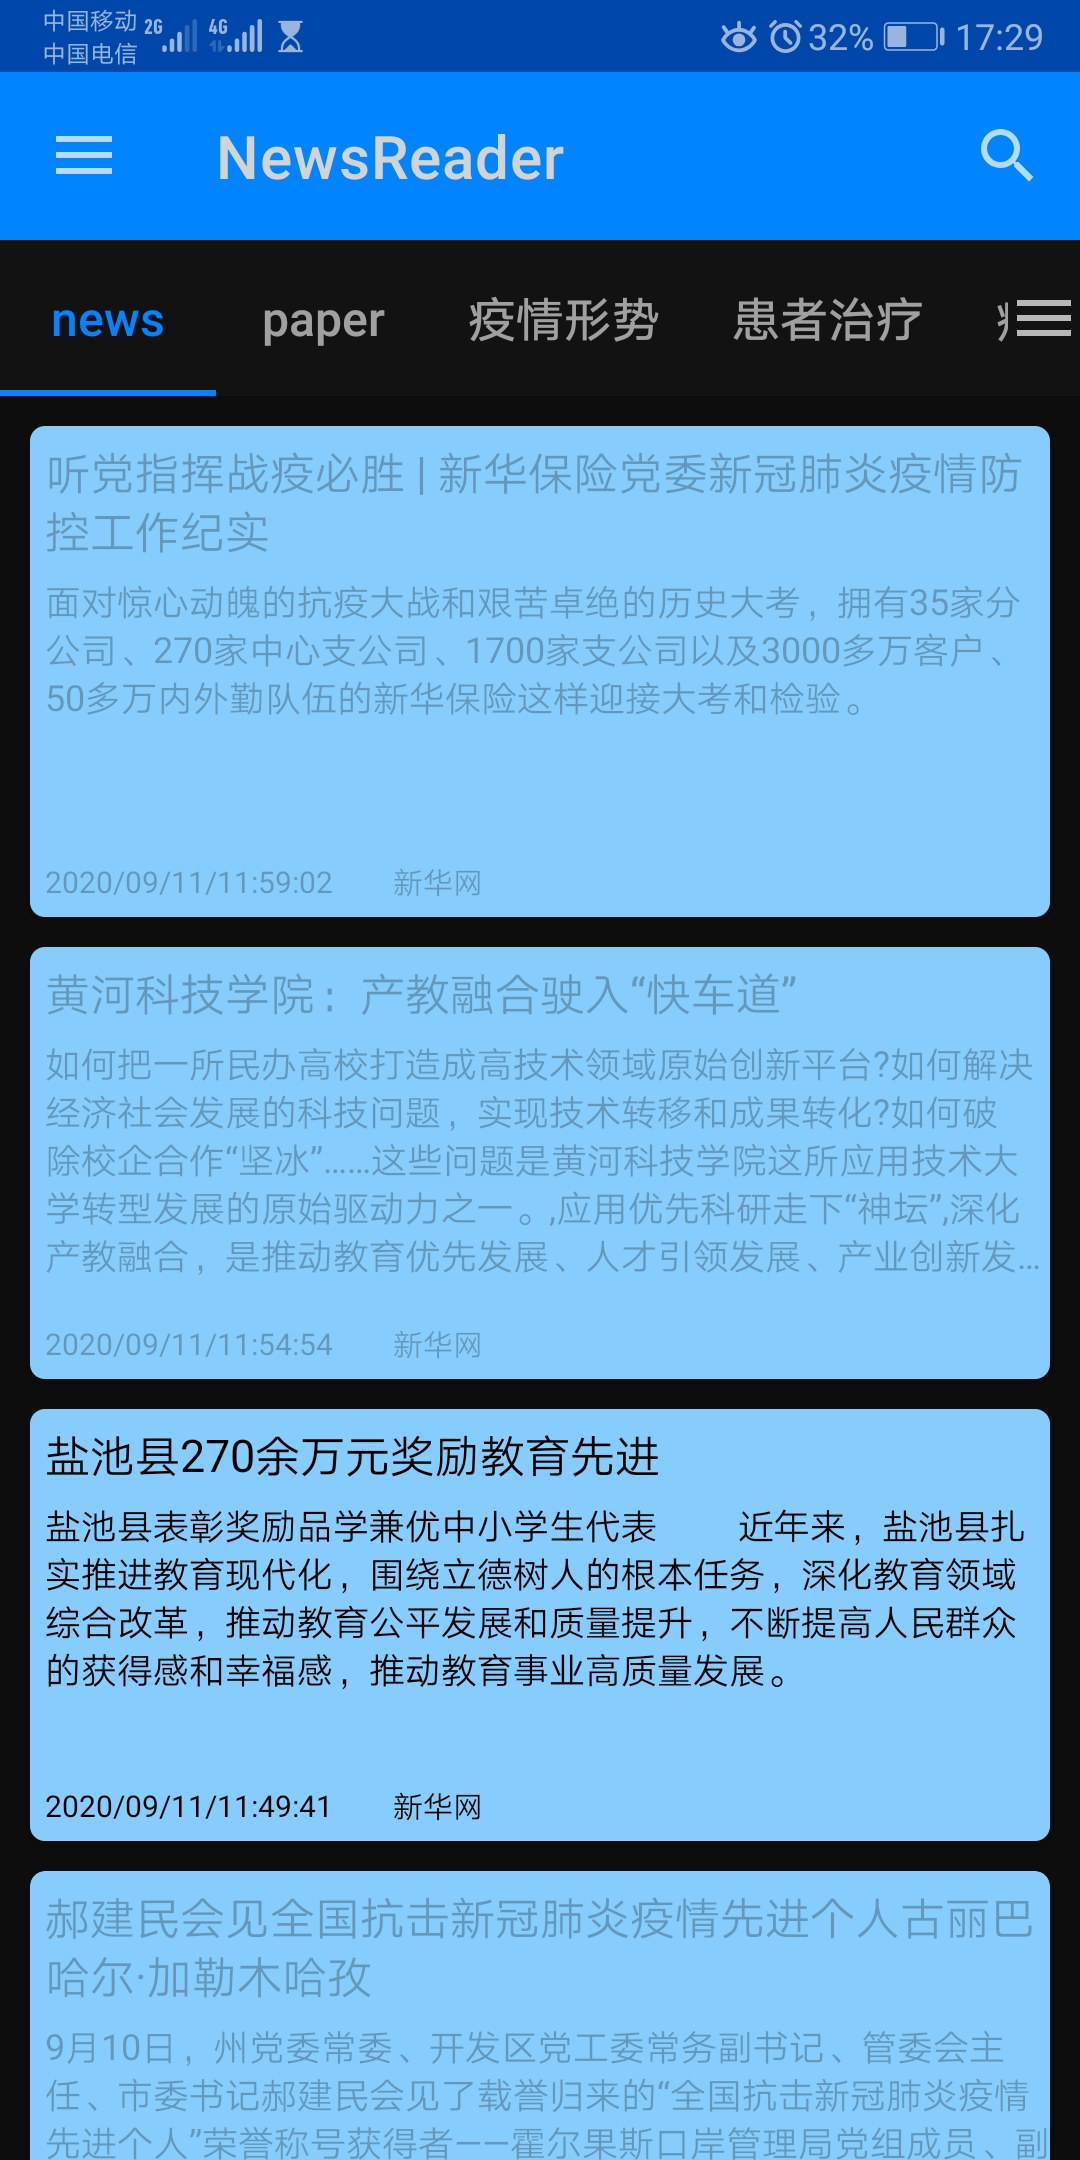
\includegraphics[width=5.5cm]{nightmode2}
%     }
%     \quad
%     \subfigure[夜间模式下实体搜索]{
%     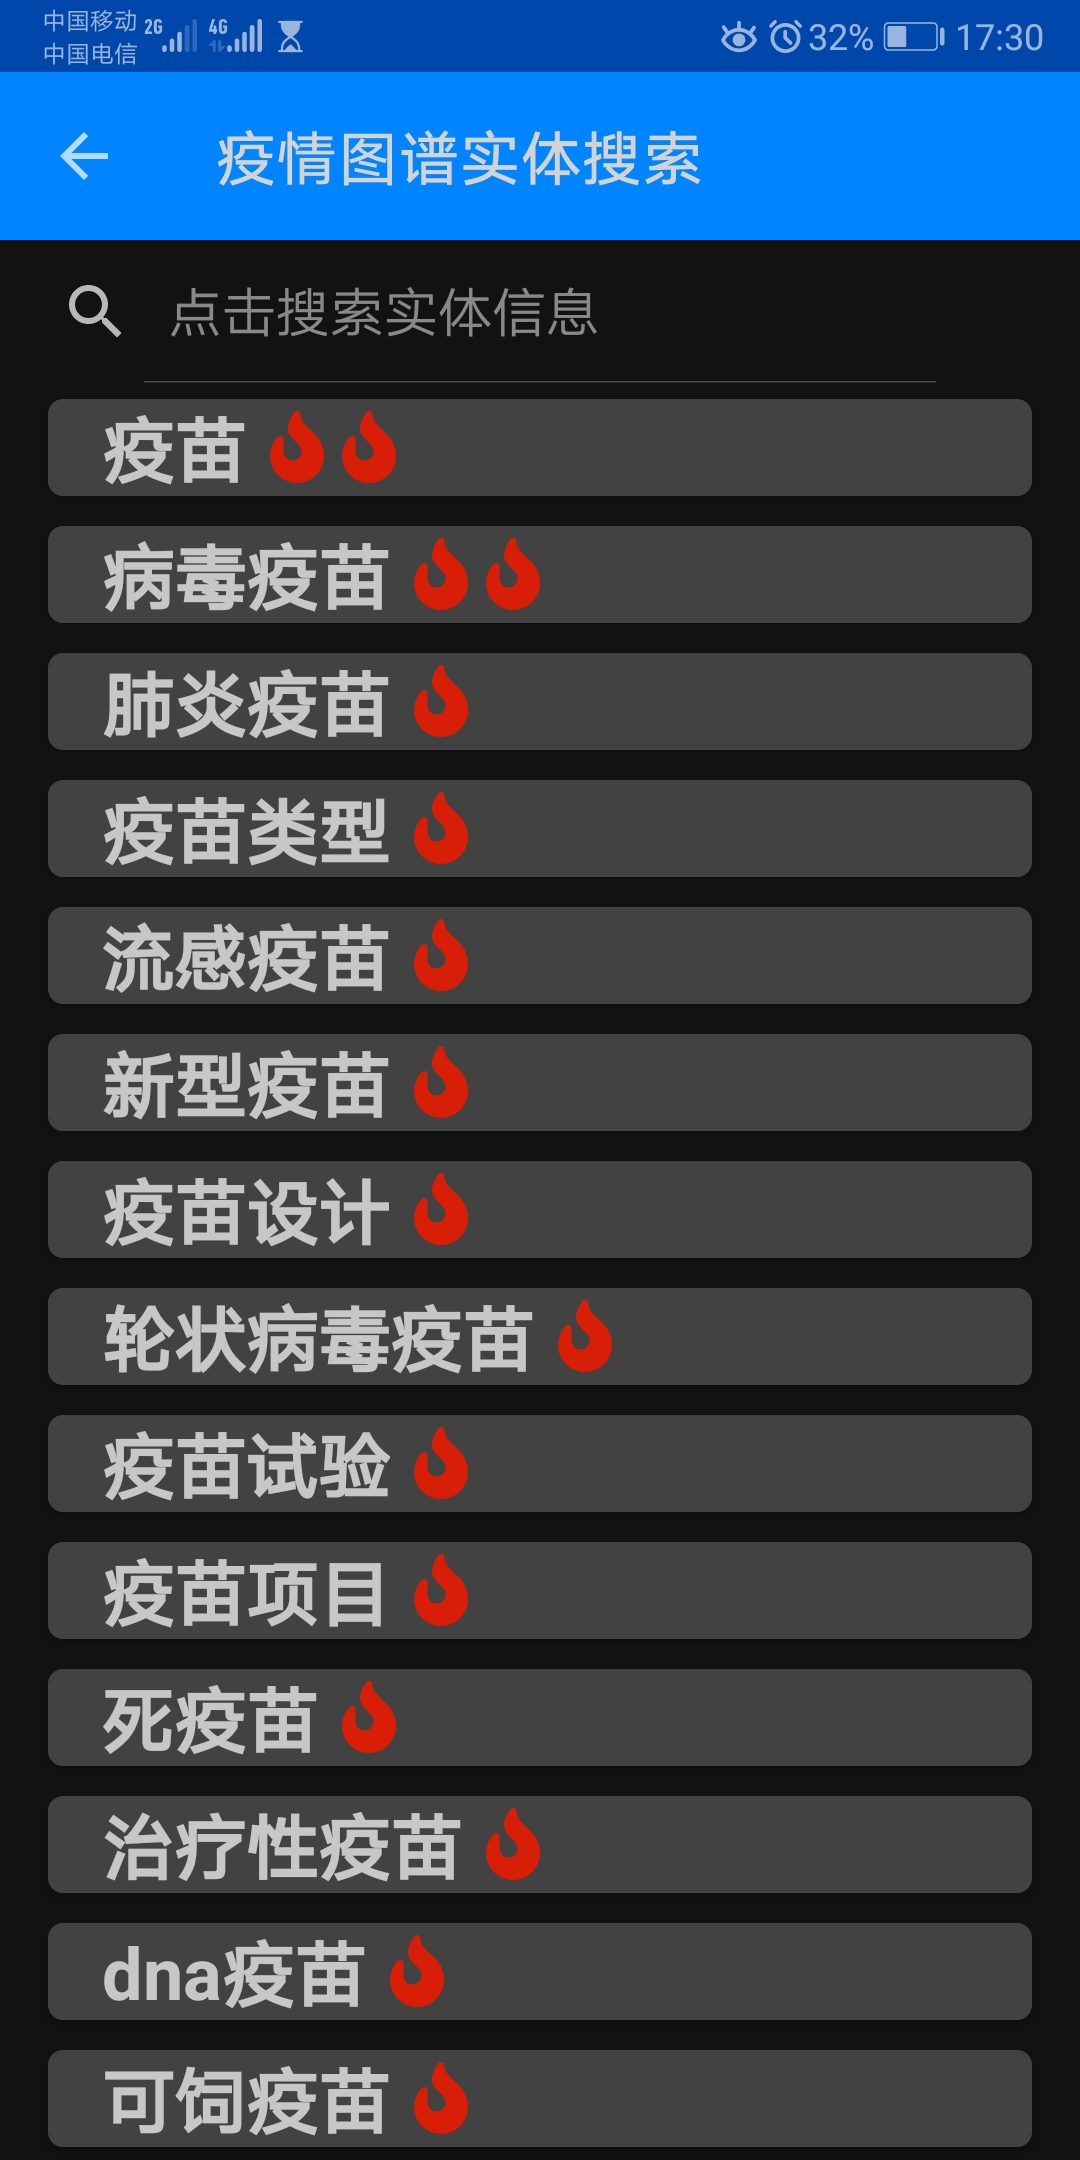
\includegraphics[width=5.5cm]{nightmode3}
%     }
%     \quad
%     \subfigure[夜间模式下知疫学者]{
%     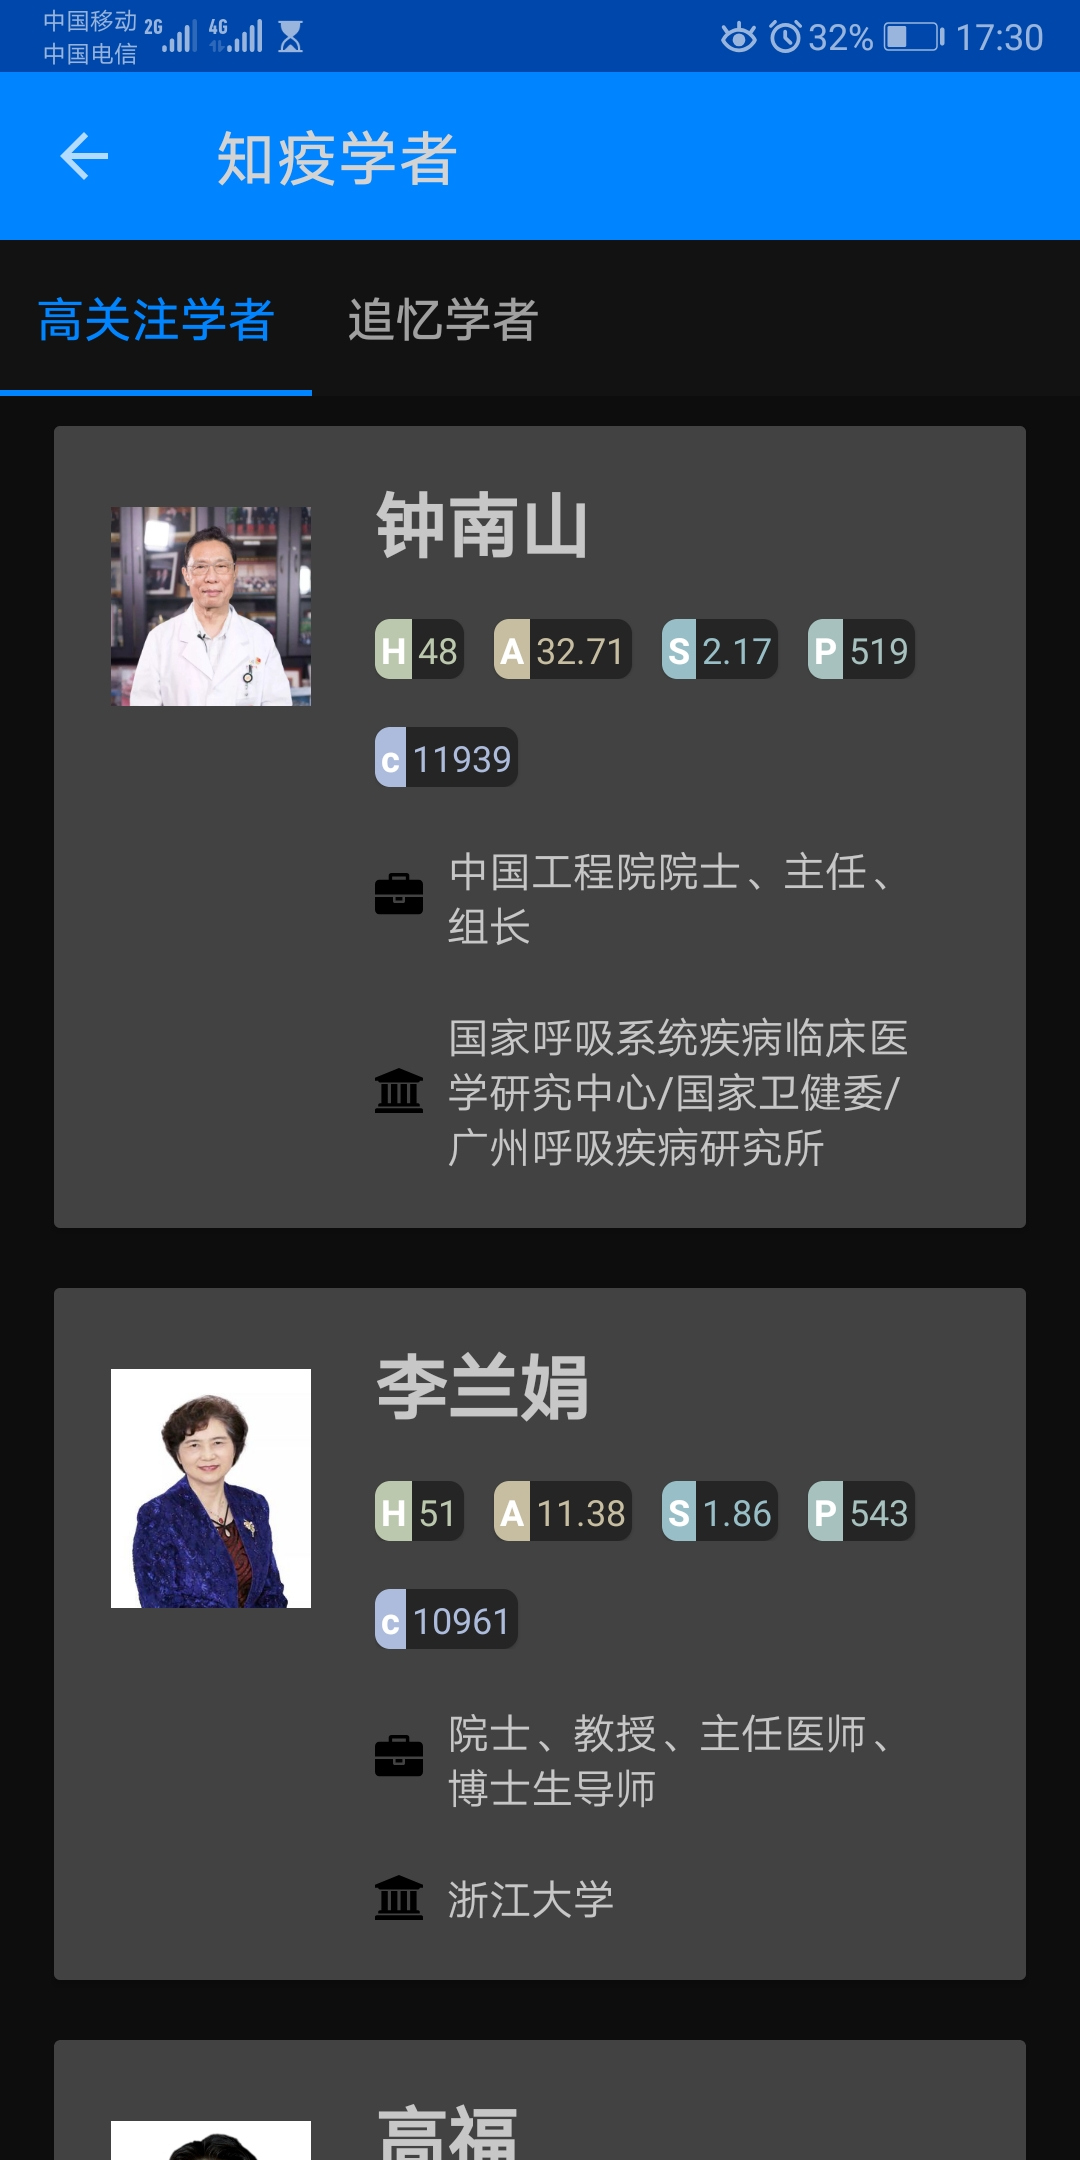
\includegraphics[width=5.5cm]{nightmode4}
%     }
%     \caption{夜间模式}
%     \end{figure}


\clearpage

\subsection{后端具体实现}
后端部分由任一完成,下面是后端的具体实现介绍。
\subsubsection{后端框架}
在对比Room, Realm等数据库之后,我们使用了Android官方推荐的Room作为后端数据库,
原因在于Google在Room数据库中,实现了很多针对Android APP开发的特性,这些特性可以简化APP的开发,同时保证数据库的高效。

\begin{figure}[htbp]
    \centering
    \label{arch}
    \subfigure[]{
    \begin{minipage}[t]{0.5\linewidth}
    \centering
    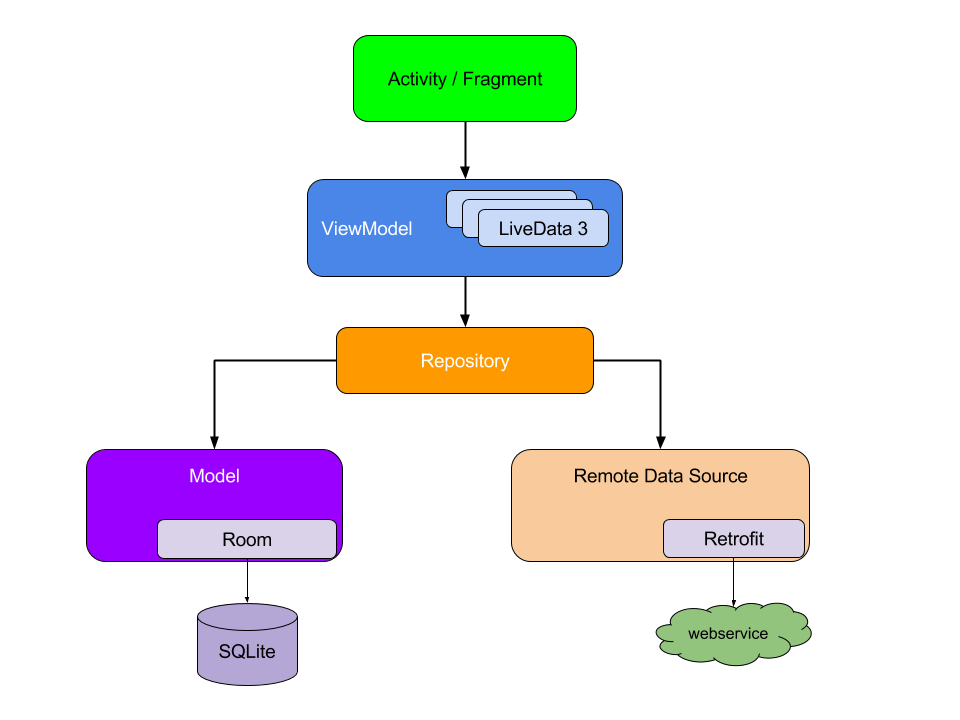
\includegraphics[width=0.8\textwidth]{archi.png}
    %\caption{fig1}
    \end{minipage}%
    }%
    \subfigure[]
    {
    \begin{minipage}[t]{0.5\linewidth}
    \centering
    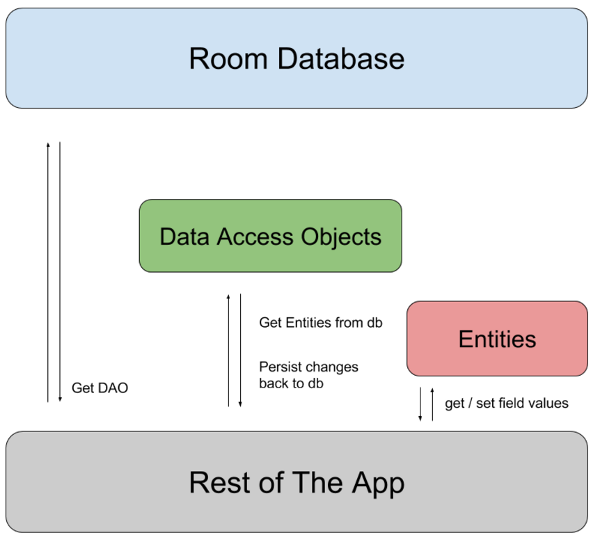
\includegraphics[width=0.8\textwidth]{archi2.png}
    %\caption{fig2}
    \end{minipage}%
    }%
    \centering
    \caption{Room数据库框架示意图}
    \end{figure}


上图展示了Room数据库的总体结构。\footnote{图源\url{https://developer.android.com/jetpack/guide}, \url{https://developer.android.google.cn/training/data-storage/room}}
在图10(a)中,我们可以看到Room数据库大体分为前端、ViewModel, Repository这几层。
前端的Activity和Fragment只需要调用ViewModel层的接口,即可通知后端对数据进行更新或
从后端获取更多内容。Repository层负责对数据进行访问,它可以通过图10(b)中的Data Access Objects(简称DAO)
对数据库进行访问,同时也可以选择从网络上请求更多数据加入数据库并显示。
这样的结构的优势在于,能够很大程度上实现前后端的解耦合。前端只调用ViewModel的接口即可获取数据,
后端复杂的逻辑全部在Repository中进行处理,降低了前后端对接的难度。

此外,这个框架中还有一个亮点,即LiveData. \footnote{关于LiveData的更多信息\url{https://developer.android.com/topic/libraries/architecture/livedata}}
LiveData很大的优点在于,能够方便地保持前端数据与后端数据的同步。例如,前端需要后端刷新新闻时,
在子线程后端数据库的确加入了最新的新闻,但前端如何知道后端数据已经更新了呢?
LiveData的作用在这里就是,在数据库层面随时监控后端的数据变化,当后端数据出现变化时,
可以立刻通知前端刷新页面,这样就保持了前后端数据的同步性。同时,LiveData在底层也处理了前端各组件生命周期、内存泄露等问题,
大大方便了开发。
\newpage
\subsubsection{数据库逻辑}
数据库主要储存了News, Paper和Events类的词条。这部分主要介绍对News和Paper词条的处理。

\begin{figure}[h]
    \label{Ratio}
    \centering
        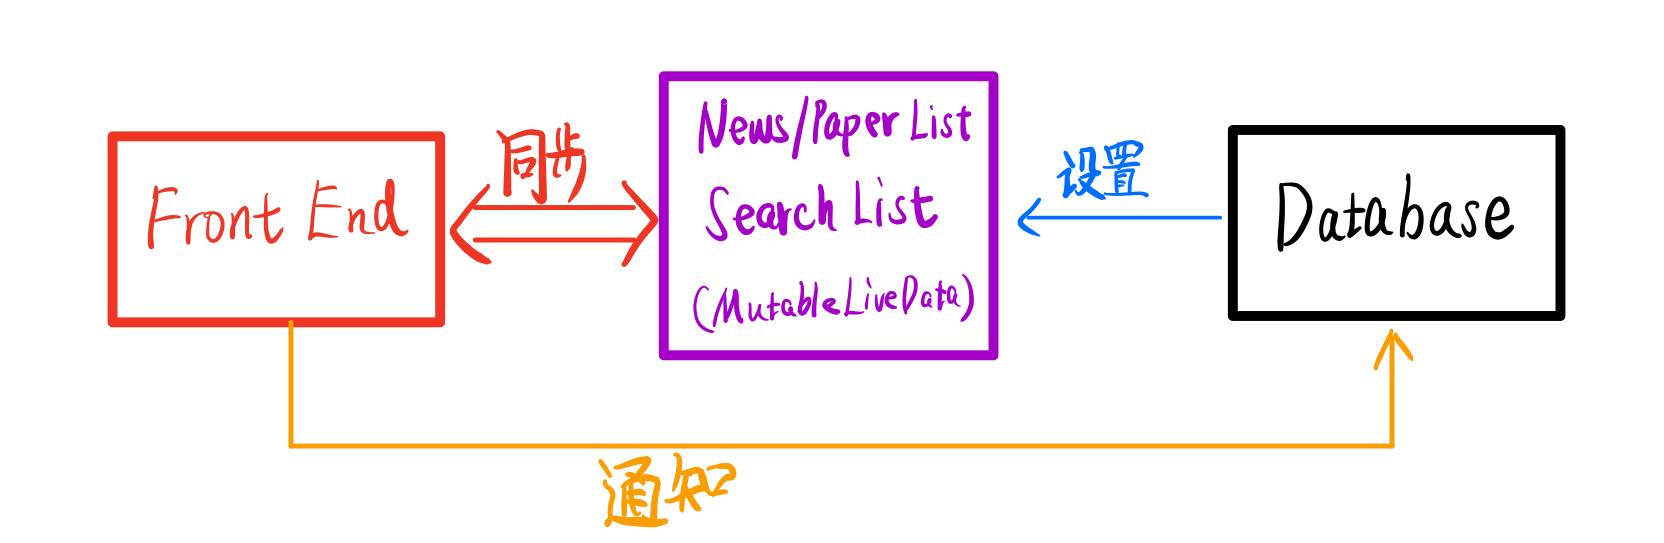
\includegraphics[width=0.8\textwidth]{db}
        \caption{News,Paper以及搜索后端处理逻辑示意图}
    \end{figure}


应用刚启动时,数据库会向API请求一个PAGE\_SIZE的news和paper数据\footnote{PAGE\_SIZE在APP中设置为100}
加入到本地的数据库中。这样应用刚启动时,数据库中就有PAGE\_SIZE数量的news和paper了。在此之后,
数据库将ADD\_SIZE条\footnote{ADD\_SIZE在APP中设置为10.}
的news和paper设置到NewsList和PaperList当中。由于NewsList和PaperList使用了
LiveData的机制,这两个List有了新的内容后,立即通知前端刷新界面,也就是说前端与LiveData就是完全同步的。

当前端上拉想要加载更多时,会告知后端。后端则会检查当前数据库中的新闻或论文是否足够给前端更多,如果仍有前端未显示的新闻,则
把尚未显示的部分加入NewsList或PaperList的LiveData中,LiveData负责与前端保持同步。若当前数据库中的新闻
不够给前端更多了,则数据库会向API请求更多的新闻或论文,加入数据库并设置LiveData,LiveData负责与前端保持同步。

当前端想要下拉刷新最新新闻时,同样会告知后端,后端则会直接向API请求最新的新闻加入数据库,并设置LiveData,LiveData负责与前端保持同步。

当前端设置想要搜索时,只需传给后端搜索关键词,后端调用SELECT语句以及LIKE子句,即可在数据库所有的news, paper和events中
匹配标题和内容,将含有相应关键词的词条设置到LiveData中,LiveData保证前端与后端返回的搜索结果同步。

当前端点击一条新闻时,会告知后端将其设置为已读状态,后端通过UPDATE语句即可设置该词条的已读状态,同样通过LiveData的机制
保证前端得到的该词条被标记为已读,以便将其显示为灰色。

这样的后端设计的优点在于:
\begin{enumerate}
    \item 简化了前端逻辑,有利于前后端解耦合。后端负责所有上拉加载更多、下拉刷新逻辑,前端只需要向后端发送请求即可。
    \item 加入LiveData作为前端与数据库中间的缓存,可实现本地新闻大量存储。如果没有LiveData作为中间的缓存,我们可能需要将数据库中的所有新闻都发给前端,这样既不必要,也会增加前端处理的难度。或者说前端每请求一次数据,后端都要到API去请求数据,这样会导致频繁的网络连接,降低APP响应速度。
            有了LiveData作为中间的缓存,我们的逻辑和实现都更为自然和简洁,APP的响应也更加快速。同时数据库可以储存大量的新闻在本地,方便离线浏览以及搜索。

\end{enumerate}

\newpage

\subsubsection{聚类逻辑}
在本APP中,我们实现了对Event类词条的在线聚类,即在APP中实时运行聚类并得到结果。
聚类用到的模型是隐含狄利克雷分布(Latent Dirichlet allocation, 简称LDA).
\footnote{感谢刘雪怡同学向我推荐了这个算法及该算法在Github上的开源代码,我使用的该算法开源代码链接为\url{https://github.com/jsksxs360/HanLDA}}

该算法的主要过程分为两个部分,训练和预测。在训练过程中,这个算法可以预先指定聚类的类个数k, 即训练出的模型可以从
训练集中学到k个类。训练集是由大量已经做好分词的文章组成的,这里对文本使用的模型是词袋模型(Bag of Words).
在训练时,该算法通过吉布斯采样的方法(或EM算法),对LDA模型的参数进行估计。训练的结果是得到k个类,每个类有20个关键词,
每个关键词都有与该类关联程度的系数。通过每个类的关键词,即可判断出该类的主题。在预测过程中,我们会计算每篇文档与模型中k个类的相似程度,选择相似程度最大的类,作为当前文档的类即可。

在我的实现中,我首先在电脑上下载了所有699条event,并对其进行分词和本地的训练。经过
我对聚类类数目的尝试,以及聚类结果的观察,设置聚类数目为5是一个合适的选择。聚类数目太多,
某些类就会太小或者与关键词的关联系数不够大,而聚类数目太少又会降低聚类的意义。

\begin{figure}[h]
    \label{Ratio}
    \centering
        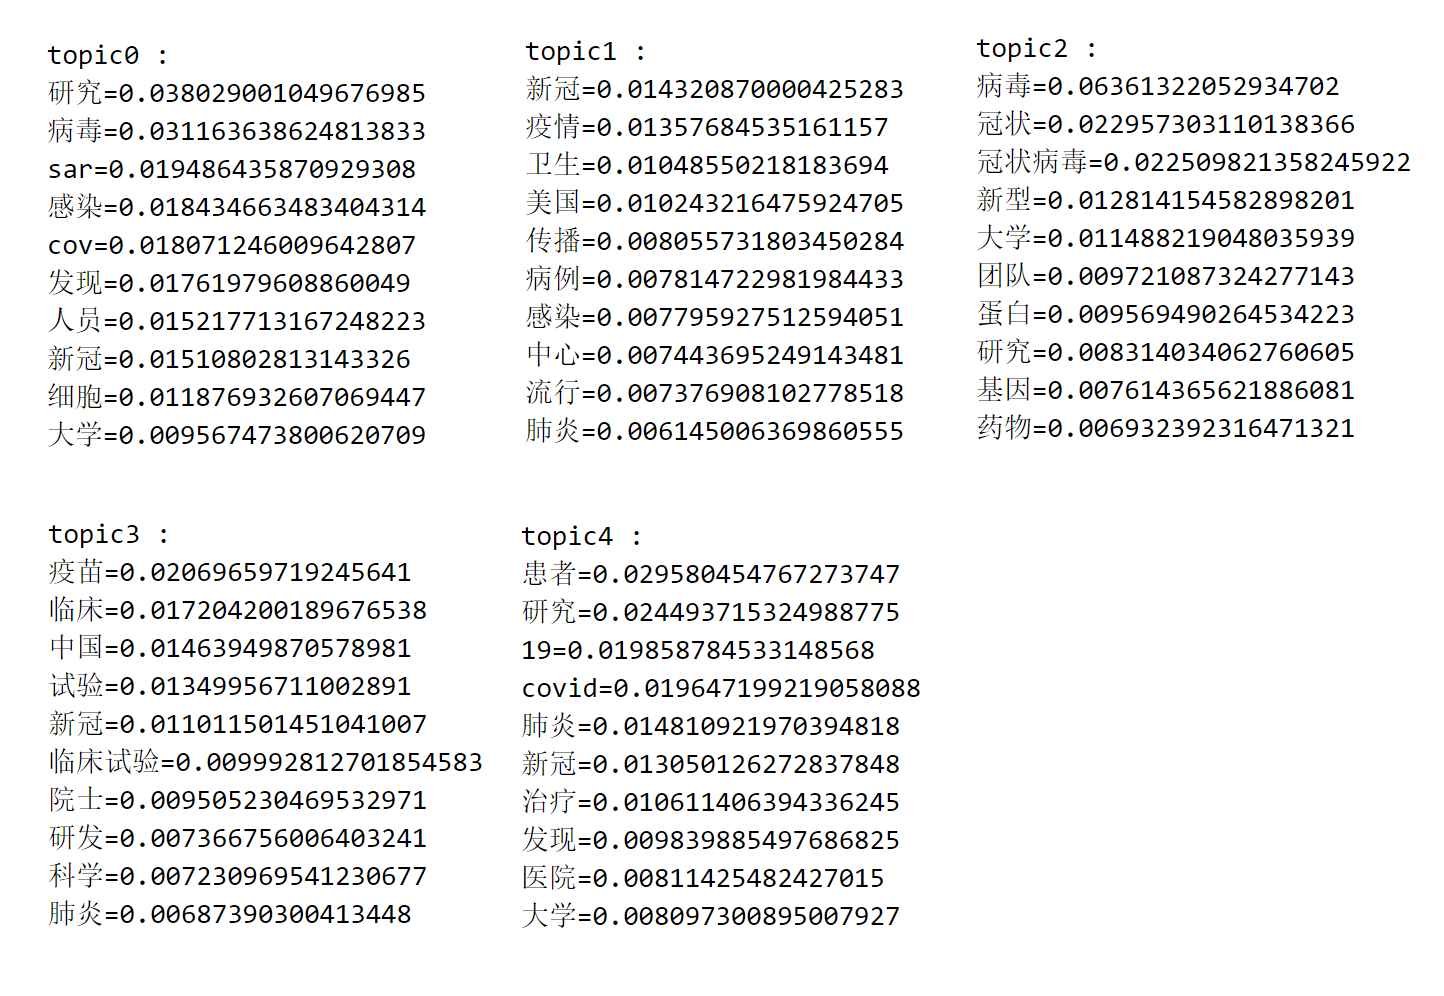
\includegraphics[width=0.6\textwidth]{cl}
        \caption{聚类训练得到各topic及topic关键词}
    \end{figure}


上图为我的聚类训练得到的topic以及topic的关键词,每个关键词后面的数字都是该关键词与这个topic的
关联系数,关联系数越大代表与topic联系越紧密。通过对这些topic关键词的观察,
我把topic0和topic2命名为"病毒研究"类,topic1命名为"疫情形势"类,topic3命名为"疫苗药物"类。
在预测时,对于一条event,我们选择其相关系数最大的topic所对应的类,作为这个event的聚类结果。


这样的聚类方法,实现了不错的结果。下表是这4类所对应的部分新闻,可以看出聚类效果很好。
\begin{table}[h]
    \caption{聚类结果分析}
    \label{tab:my-table}
    \centering
    % \resizebox{!}{4cm} {

    \begin{tabular}{|l|l|}
    \hline
                          & 内容                                                                                                                          \\ \hline
    \multirow{2}{*}{病毒研究} & \begin{tabular}[c]{@{}l@{}}杜兰大学医学院罗伯特・加里教授等研究发现新型病毒不是在实验室中构建的,\\      也不是有目的性的人为操控的病毒,而是是自然产生的。\end{tabular}                \\ \cline{2-2} 
                          & \begin{tabular}[c]{@{}l@{}}deCODE基因公司通过对冰岛确诊病例进行基因测序分析,发现40个新冠病毒的变体。\\      病毒学家认为新冠病毒最终可能会进化为更具传染性但低致病性的病毒\end{tabular}    \\ \hline
    \multirow{2}{*}{疫苗药物} & \begin{tabular}[c]{@{}l@{}}上海市科委主任张全称在疫苗研发方面,多路线部署推进的疫苗研发均取得良好进展。\\      mRNA疫苗,已启动灵长类动物毒理和药效预实验,预计4月中旬临床试验\end{tabular}    \\ \cline{2-2} 
                          & \begin{tabular}[c]{@{}l@{}}以色列科技部27日宣布,该国研究人员正在加快开发一种口服的新型冠状病毒疫苗,\\      研究人员希望能在8到10周内制造出疫苗,有望在90天内开始临床试验。\end{tabular}    \\ \hline
    \multirow{2}{*}{疫情形势} & \begin{tabular}[c]{@{}l@{}}国家卫健委新闻发言人米锋介绍,目前国内疫情防控形势持续向好,但是\\      境外疫情却在加速扩散,“外防输入”已经成为当前我国疫情防控的重中之重。\end{tabular}         \\ \cline{2-2} 
                          & \begin{tabular}[c]{@{}l@{}}首都机场设置处置专区,全部国际及来自港澳台地区进港航班,均停靠首都机场处置专区,\\      3月16日起所有境外进京人员均需转送至集中观察点隔离观察14天\end{tabular}     \\ \hline
    \multirow{2}{*}{患者治疗} & \begin{tabular}[c]{@{}l@{}}托珠单抗(Tocilizumab)对重症COVID-19患者临床验证有效果,其机制是\\      阻断IL-6抑制炎症因子风暴,由于病人数量有限,后续仍需大量研究。\end{tabular} \\ \cline{2-2} 
                          & \begin{tabular}[c]{@{}l@{}}首都医科大学附属北京同仁医院发表文章指出高龄和男性是COVID-19预后\\      较差的危险因素,男性更倾向于具有更高的疾病程度和死亡率。\end{tabular}            \\ \hline
    \end{tabular}
    % }
    \end{table}

聚类这部分实现的难点有以下两点:
\begin{enumerate}
    \item 弄懂LDA的聚类原理。\footnote{学习时主要参考了\url{https://en.wikipedia.org/wiki/Latent_Dirichlet_allocation}} LDA的数学原理较为复杂,需要详细的学习才能使用。
    \item 与开源代码做对接。我参考的开源LDA实现\footnote{参考了\url{https://github.com/jsksxs360/HanLDA}},是通过绝对路径访问文件中的内容作为输入进行预测的,此外该开源代码也只能从绝对路径加载训练好的模型,无法直接移植到Android APP中。
          因此,我对这份开源代码也进行了一定的学习,修改了文件的推断函数使之可以将字符串作为输入,并且学习在Android APP中加载本地文件,同时修改开源代码的构造函数使之成功适配Android APP.\footnote{此处参考了\url{https://stackoverflow.com/questions/34521349/asset-file-directory-giving-java-io-filenotfoundexception-eclipse}的第一个回答.}
\end{enumerate}

\subsubsection{其他逻辑}
其他后端的需求主要有疫情数据、疫情图谱和知疫学者的逻辑。
这部分的处理逻辑与news和paper的逻辑相仿。但由于疫情数据、疫情图谱、知疫学者具有较强的时效性和灵活性,
不便像news和paper一样,做本地的大量存储。因此每次调用这些功能,都会向API发送请求,API返回数据后设置LiveData,
LiveData保证前端同步显示。因此这部分在显示时,可能会先空白1-2s,然后再显示,这是后端在向API请求数据并解析数据的时间。
% \begin{figure}[h]
%     \label{Ratio}
%     \centering
%     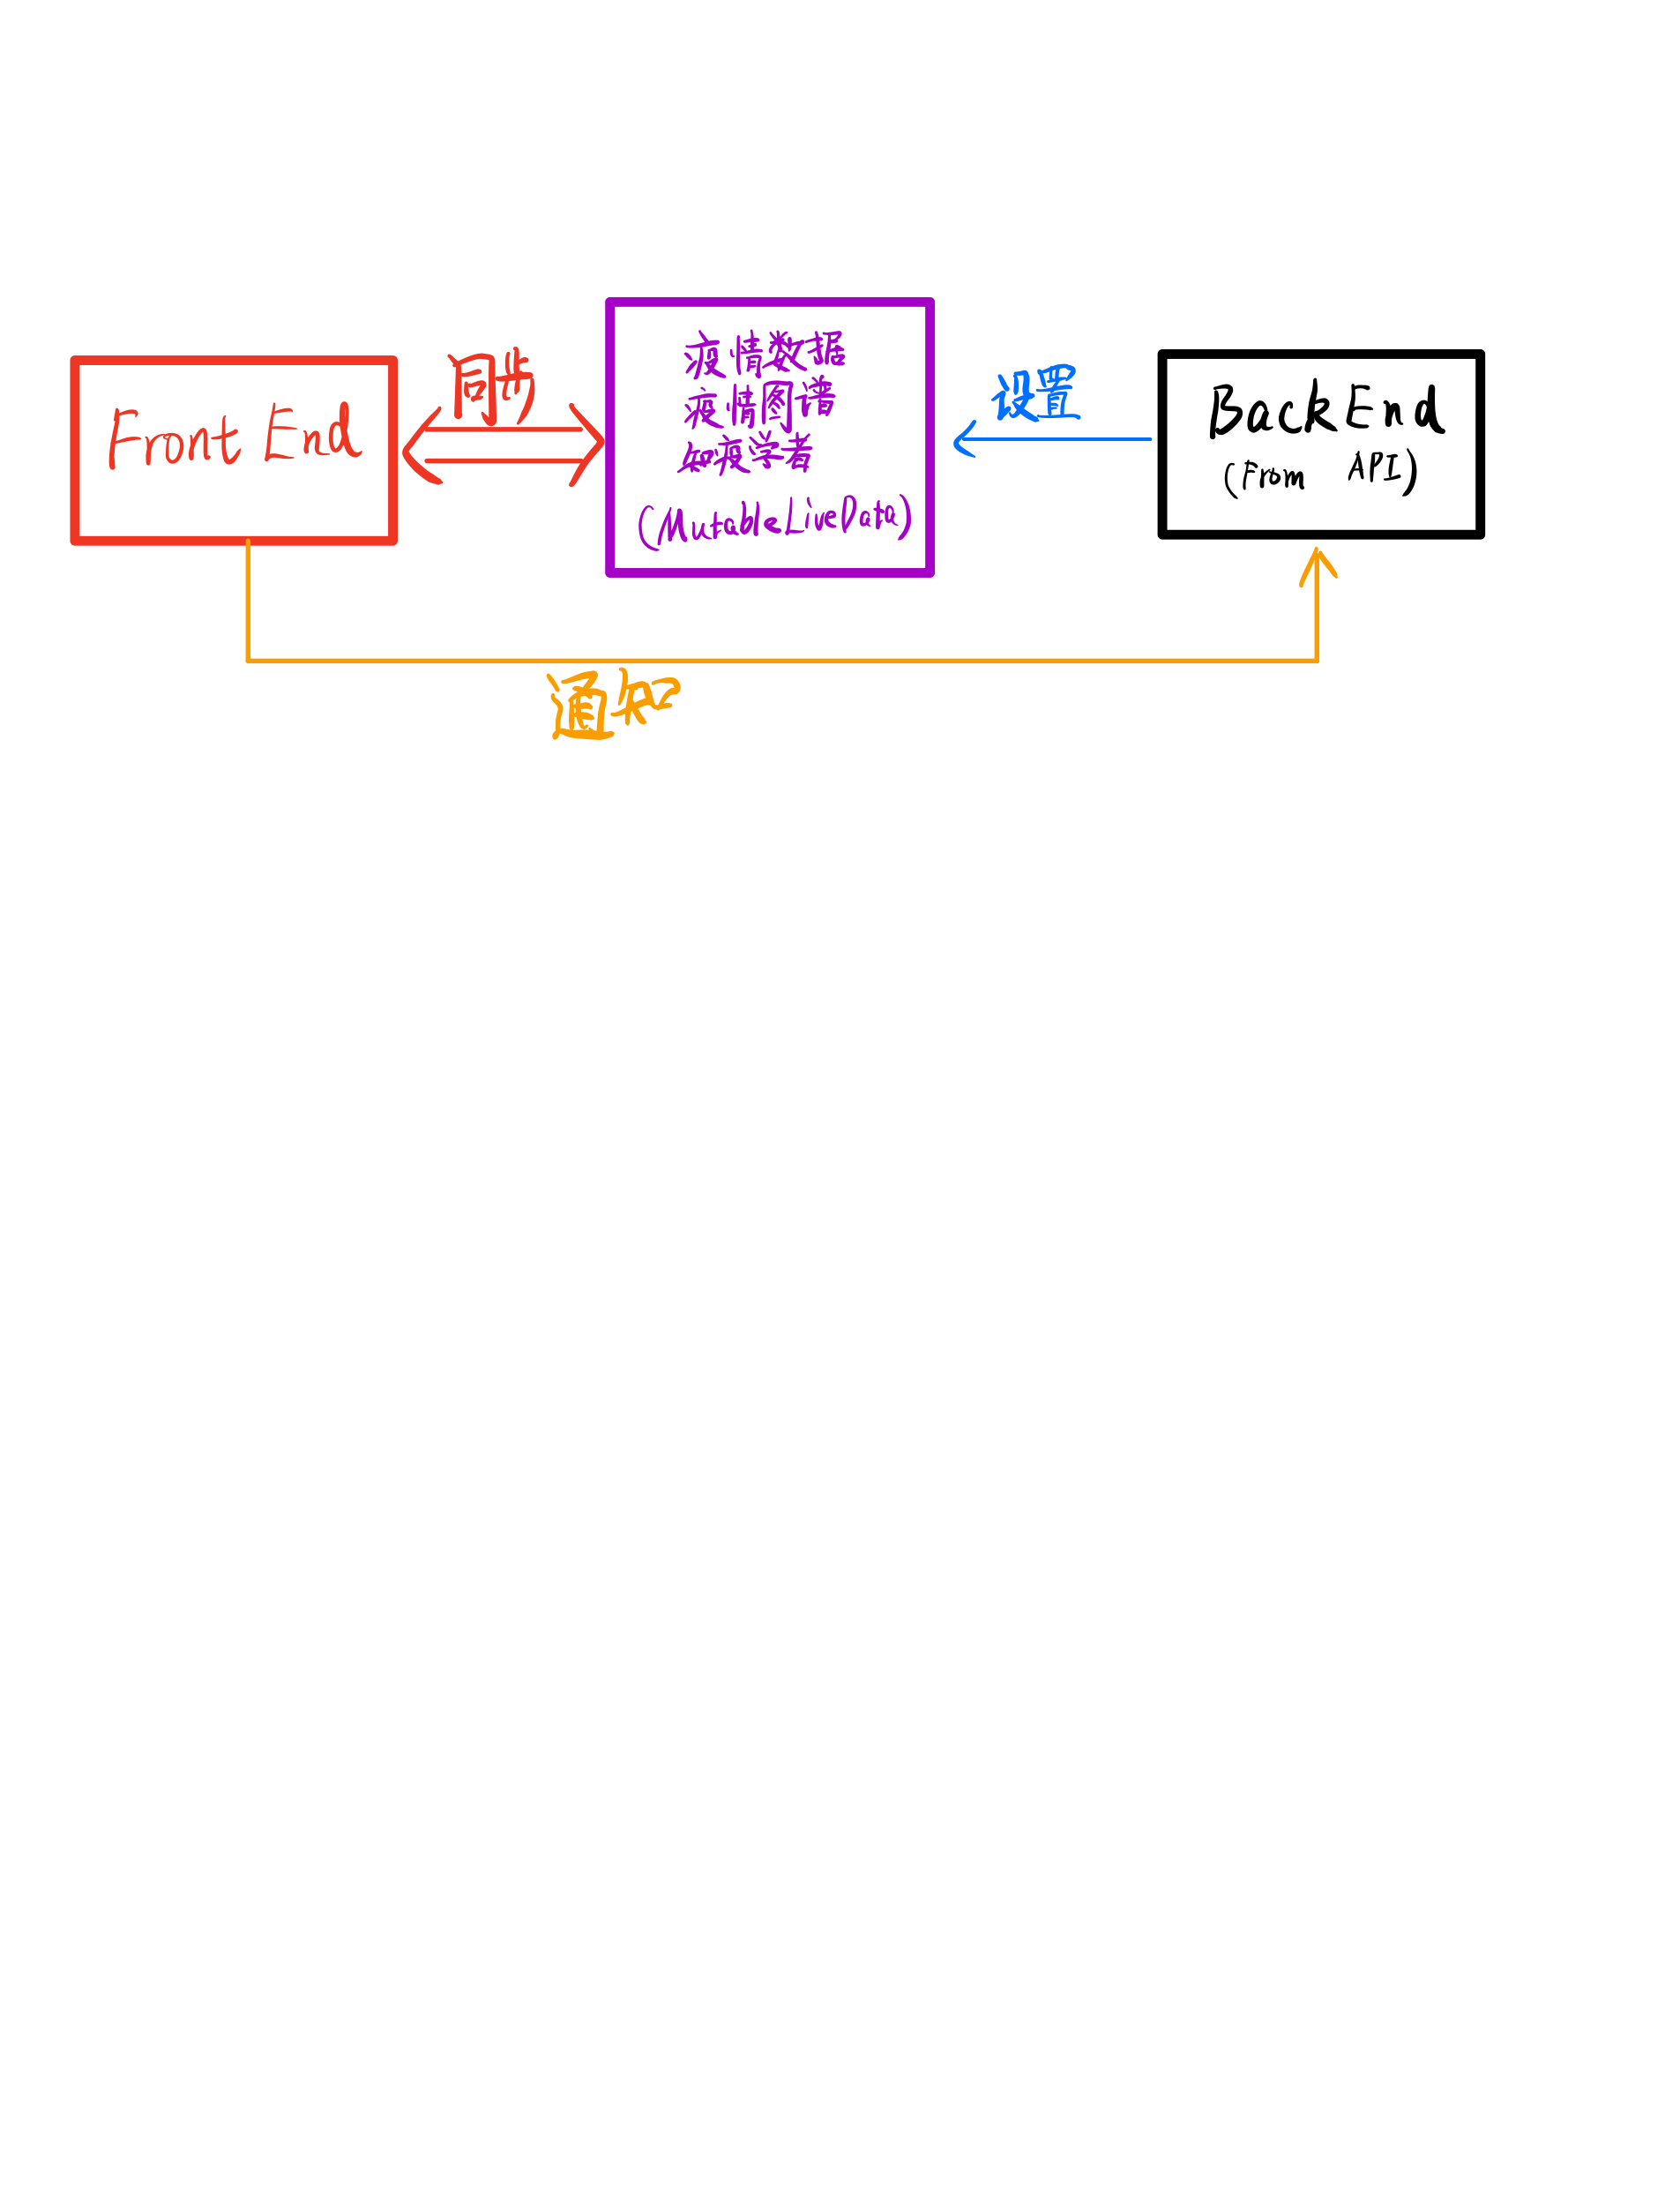
\includegraphics[width=0.5\textwidth]{other}
%     \caption{疫情数据, 疫情图谱, 知疫学者后端逻辑}
% \end{figure}

\newpage
\section{总结与心得}
\subsection{前端部分总结与心得-刘畅}
本次大作业中我负责前端部分,最大的收获是java编程能力和前端开发能力得到了一定的提高。
另外,快速获得所需要的学习资料、快速习得其中的要领、快速定位问题出现的位置是每一个开发者必备的能力。
我认为本次开发可以起到锻炼这些能力的效果。另外还要特别感谢后端队友精妙的框架设计,让我能够专注地进行前端开发,解决了前端开发的后顾之忧。
队友的出色和靠谱表现让我印象非常深刻。

\subsection{后端部分总结与心得-任一}
在本次项目中,我负责了后端的设计,主要内容是设计数据库的组织结构、设计后端与前端的交互方式。
得益于LiveData的功能,我们基本没有在前后端数据同步上花费过多精力,得益于Room数据库官方推荐的
组织结构,整个项目的前后端分离也做的非常完善。\footnote{参考了Room的组织架构教程\url{https://codelabs.developers.google.com/codelabs/android-room-with-a-view/#0}}
总体来说开发体验非常好!
虽然说由于这是我第一次设计后端,在一开始的结构选择上也有过犹豫和反复,但最后还是选择了
FrontEnd-LiveData-Database这样的逻辑来展示news和paper,这样的结构有着很好的性能。

整个项目的进度我们也把握得很合理。在小学期第4周刚开始,我们在正常小学期课业与考试的
压力中,从9月3日-9月6日进行了4天高强度的开发,每天工作时间在6-8小时,这段时间我们就基本完成了所有的
基础功能和一部分扩展功能。9月10日中午,我们就全面完成了基础功能和扩展功能,在当天下午进行了充分的测试和调优,保证了APP的稳定性。
9月11日提交当天,我们录制了展示视频、撰写实验报告,整个过程很艰辛,但进度非常稳健。

在这里我还想特别感谢我的队友刘畅。她是一位非常优秀、努力、认真并且可靠的合作伙伴。她在小学期开始第一周
就完成了简要的前端框架,在之后的时间里一直对前端进行调优和增加新功能,她对这个项目的投入让我十分敬佩。
此外也感谢老师和助教对我们的悉心指导和帮助。最后也感谢努力的自己,设计了一个不错的后端,让整个APP的效率和鲁棒性都很好,
也希望我自己之后继续努力,进一步增强自己的工程能力。


% \section{实验概述}
% 本次作业中,我通过所学的CUDA编程知识,结合对GPU架构的理解,实现了优于baseline的
% gemm算法,即计算$C=\alpha AB+\beta C$, 其中$A, B, C$的矩阵大小分别为$M\times K, K\times N, M\times N$.
% 我做的优化也主要集中于$AB$的矩阵乘法运算。
% 提交目录中的gemm\_2018011423.h即为我实现的gemm算法头文件。

% \section{实验思路}
% 本次实验中,我主要利用了GPU每个block中的shared memory,来减少从global memory中
% 读取数据,以加快矩阵乘法计算速度。

% 具体来说,我将每个block的形状设置为32 * 32,对于每个待计算的Block,令Block中的每个Thread都从
% 当前Block计算所涉及的
% A矩阵和B矩阵中的某一部分,
% 读取相应的一个元素到A\_shared和B\_shared这样的shared memory中的矩阵里面。
% 由于shared memory大小有限,我固定A\_shared和B\_shared矩阵的大小均为32 * 32.
% 这样就需要在一个Block的计算中,对涉及的A矩阵和B矩阵的某一部分进行循环遍历,每次遍历都需要更新A\_shared和
% B\_shared中的数据,以得到最终该Block内元素的计算结果。
% 实现示意图如图1(b)所示\footnote{图源\url{https://docs.nvidia.com/cuda/cuda-c-programming-guide/#shared-memory}}。

% \begin{figure}[htbp]
%     \centering
%     \subfigure[baseline的实现方法]{
%     \begin{minipage}[t]{0.5\linewidth}
%     \centering
%     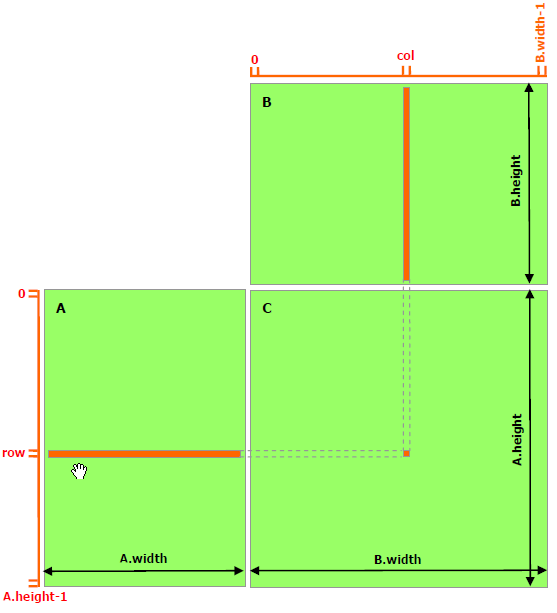
\includegraphics[width=0.8\textwidth]{base.png}
%     %\caption{fig1}
%     \end{minipage}%
%     }%
%     \subfigure[我的实现方法]{
%     \begin{minipage}[t]{0.5\linewidth}
%     \centering
%     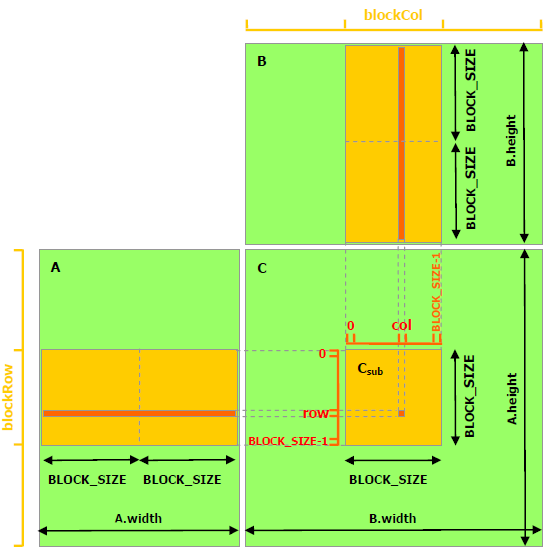
\includegraphics[width=0.8\textwidth]{my.png}
%     %\caption{fig2}
%     \end{minipage}%
%     }%
%     \centering
%     \caption{baseline实现方法与我的实现方法对比}
%     \end{figure}

%     \begin{figure}[h]
%         \label{Ratio}
%         \centering
%             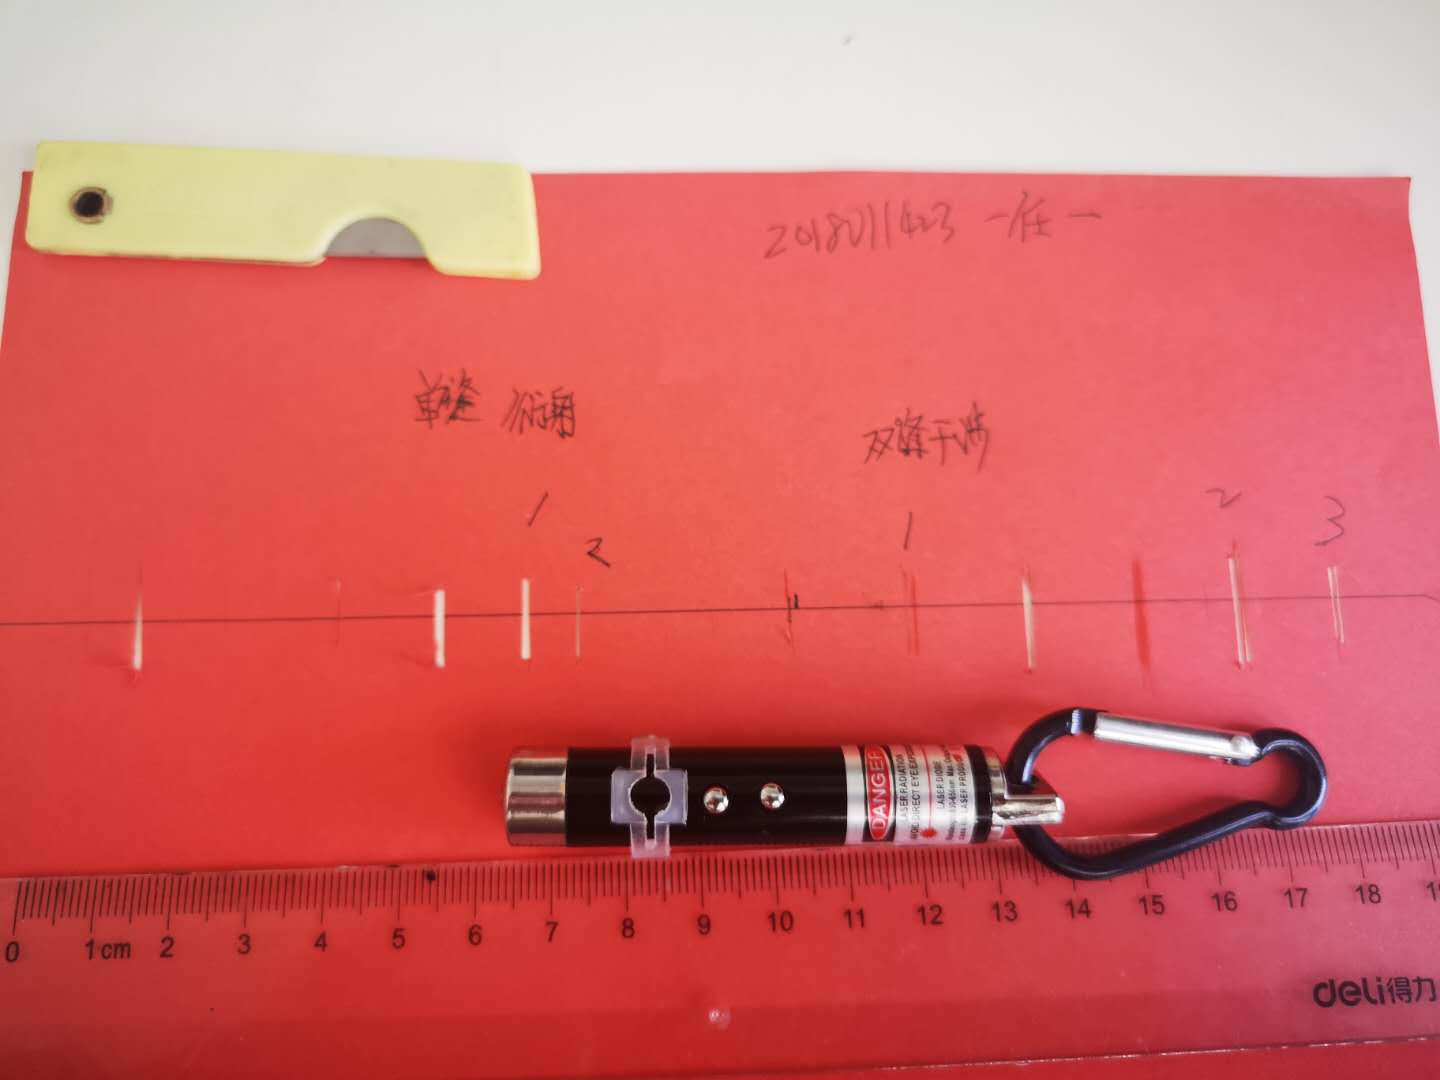
\includegraphics[width=0.7\textwidth]{fc.jpg}
%             \caption{主要实验器材一览}
%         \end{figure}
    
%         \begin{figure}[h]
%             \centering
%             \subfigure[激光照射单缝]{
%             \includegraphics[width=5.5cm]{fc1.jpg}
%             }
%             \quad
%             \subfigure[实验背面图]{
%             \includegraphics[width=5.5cm]{fc2.jpg}
%             }
%             \quad
%             \subfigure[用小刀刻出的单缝和双缝]{
%             \includegraphics[width=5.5cm]{fc3.jpg}
%             }
%             \quad
%             \subfigure[实验正面图]{
%             \includegraphics[width=5.5cm]{fc4.jpg}
%             }
%             \caption{实验装置图}
%             \end{figure}
%             \begin{figure}[h]
%                 \label{Ratio}
%                 \centering
%                     \includegraphics[width=0.5\textwidth]{feng.jpg}
%                     \caption{纸上各单缝与双缝展示图}
%                 \end{figure}
% \newpage
% \section{实验中的改进思路}
% 本部分中我将介绍在进行本实验的过程中,我的一些想法和改进思路。
% \subsection{使用动态分配的shared memory,难以突破shared memory大小的瓶颈}
% 当我对整个实验框架和baseline的实现思路进行学习后,我认为baseline
% 很慢的很大一部分原因在于,没有使用shared memory,每个线程只是从global memory当中读取数据,
% 这样就没有很好地利用GPU的体系结构。

% 一个最直观的改进想法是,将实验中用到的矩阵$A,B,C$都存在shared memory中.
% 但经过资料的查找,我发现实验平台上GPU的shared memory大小为48KB
% \footnote{资料来源于\url{https://devblogs.nvidia.com/using-shared-memory-cuda-cc/}},
% 这样小的存储空间难以
% 存下$A,B,C$这3个矩阵,同时也不利于任意大小矩阵的计算。

% 为了减少对shared memory大小的占用,我发现每个Block在计算的过程中,
% 只需要$A, B$矩阵的一部分内容,即可完成Block内的元素计算。
% 举例来说,使用框架最初默认的$32\times 8$的Block大小,
% $M=300, N=400, K=500$. 在这样的参数下,每个Block所需要矩阵$A$中$8\times K=4000$个元素,
% 需要矩阵$B$中$32\times K=16000$个元素,总计需要$20000$个元素。每个double型变量大小为8Byte,
% 因此该Block需要的元素所占的空间为160KB, 这比shared memory的48KB要大,因此不可行。
% 此外这个数字还依赖于$K$的大小,也不利于任意大小矩阵的计算。

% \subsection{固定所需的shared memory大小,效果较好}
% 为了解决该问题中,shared memory大小有限带来的瓶颈,我上网查阅了一些资料,在Nvidia官方文档中找到了
% 较为合适的解决方案
% \footnote{参考了Nvidia文档\url{https://docs.nvidia.com/cuda/cuda-c-programming-guide/#shared-memory}}
% ,并参考官方的解决方法,顺利完成了该实验,并得到了优于baseline的较好的结果。

% 具体来说,shared memory一次难以存下每个Block所需的矩阵元素,一个解决方法就是
% 固定每次shared memory存储的元素个数,分多次将所需的矩阵元素放入shared memory中进行计算。示意图如图1(b)所示。
% 使用这个方法可以充分利用GPU中的shared memory, 同时也巧妙地解决了shared memory大小有限的问题,并且该解决方案也不依赖于输入矩阵的大小,具有很强的灵活性。
% 不过该算法对于$M, N, K$不被Block大小整除的情况,需要一些特殊处理,
% 经过一定的调试,我也完成了对该情况的处理,从而能够处理任意大小矩阵的乘法运算,
% \clearpage
% 为了进一步优化该算法,我试图调整每个Block的大小,从$16\times 16$调整到了$32\times 32$.
% 在$M=978, N=782, K=633$的double型运算中,
% 得到的实验结果如下表:
% \begin{table}[h]
%     \caption{使用不同大小的BlockSize对性能的影响}
%     \label{tab:my-table}
%     \centering
%     \begin{tabular}{|l|c|c|c|}
%     \hline
%      & \multicolumn{1}{l|}{time(s)} & \multicolumn{1}{l|}{GFLOPS} & \multicolumn{1}{l|}{SpeedUp Ratio} \\ \hline
%     BlockSize=16 & 0.005441 & 177.94 & 2.50  \\ \hline
%     BlockSize=32 & 0.004417 & 219.20 & 3.09  \\ \hline
%     Cublas       & 0.001247 & 776.36 & 10.95 \\ \hline
%     Baseline     & 0.013540 & 70.91  & 1.00  \\ \hline
%     \end{tabular}
%     \end{table}
% 从表中可以看出,我实现的算法性能较baseline有很大的提升,此外BlockSize较大时性能相较BlockSize较小时的性能更好。
% 这让我思考上面两个现象的原因。我从对global memory读取次数角度,来看我的算法相较baseline算法的提升之处,以及BlockSize对算法性能的影响。

% 为了分析的简便起见,我们在分析时认为$M, N, K$都可以被BlockSize整除,且仅考虑矩阵乘法的部分(即$C=AB$两个矩阵的乘法).
% 对于baseline算法来说,$C$中每个元素的计算,都需要从global memory中读取所需的元素。
% $C$中每个元素的计算需要$A, B$两个矩阵中的$2\times K$个元素,$C$中共有$M\times N$个元素.
% 因此使用baseline算法,共需从global memory中读取$2MNK$个元素.

% 对于我的算法来说,$C$中每个Block需要从global memory中读取$2\times BlockSize\times K$个元素,
% $C$中共有$\frac{MN}{BlockSize^2}$个Block. 因此使用我的方法需要从global memory中读取
% $\frac{2MNK}{BlockSize}$个元素,需要从global memory中读取的元素少于Baseline算法。

% 由上面的分析,相较baseline算法,我的算法可以显著降低从global memory读取元素的次数,且从global memory中读取元素的个数与
% BlockSize成反比。这样就可以很好地解释在表1的实验中的两个实验现象,即我实现的算法性能较baseline有很大的提升,
% 以及BlockSize较大时性能相较BlockSize较小时的性能更好。


% \newpage
% \section{实验结果分析}
% 本部分中,我将通过不同尺寸的矩阵,对我的算法进行充分的性能测试,并与Cublas和Baseline算法进行对比分析。
% 在表格和图中,MyGemm-16和MyGemm-32分别表示BlockSize为16和32的我的算法。为了展示清晰,图中的横坐标均为以2为底的对数坐标。
% 在如下所有测试中,我的算法结果均与正确结果保持一致。

% \subsection{固定$K$, 改变$M, N$}
% 在本部分测试时,为了方便起见,我令$K=1024$, $M=N=Matrix Order$.得到性能分析图表如下:
% \begin{table}[h]
%     \centering
%     \caption{GFLOPS-矩阵阶数表}
%     \label{tab:my-table}
%     \begin{tabular}{|l|r|r|r|r|r|r|r|}
%     \hline
%     MatrixOrder & 4     & 32     & 128     & 512     & 2048     & 8192     & 16384    \\ \hline
%     Baseline    & 0.172 & 9.982  & 61.494  & 77.081  & 78.642   & 78.363   & 78.397   \\ \hline
%     MyGemm-16   & 0.253 & 14.306 & 132.436 & 193.081 & 204.026  & 203.275  & 203.108  \\ \hline
%     MyGemm-32   & 0.286 & 10.821 & 110.799 & 223.122 & 236.552  & 237.245  & 237.023  \\ \hline
%     Cublas      & 0.109 & 7.081  & 109.683 & 702.897 & 1044.848 & 1078.783 & 1079.668 \\ \hline
%     \end{tabular}
%     \end{table}
%     \begin{table}[h]
%         \caption{加速比-矩阵阶数表}
%         \label{tab:my-table}
%     \centering

%         \begin{tabular}{|l|r|r|r|r|r|r|r|}
%         \hline
%         MatrixOrder & 4        & 32       & 128      & 512      & 2048      & 8192      & 16384     \\ \hline
%         MyGemm-16   & 1.469 & 1.433 & 2.153 & 2.504 & 2.594 & 2.594 & 2.591 \\ \hline
%         MyGemm-32   & 1.660    & 1.084    & 1.802    & 2.895    & 3.008     & 3.028     & 3.023     \\ \hline
%         Cublas      & 0.631    & 0.709    & 1.784    & 9.119    & 13.286    & 13.767    & 13.772    \\ \hline
%         \end{tabular}
%         \end{table}
% \begin{figure}[htbp]
%     \centering
%     \subfigure[GFLOPS与矩阵阶数折线图]{
%     \begin{minipage}[t]{0.5\linewidth}
%     \centering
%     \includegraphics[width=\textwidth]{gm.png}
%     %\caption{fig1}
%     \end{minipage}%
%     }%
%     \subfigure[加速比与矩阵阶数折线图]{
%     \begin{minipage}[t]{0.5\linewidth}
%     \centering
%     \includegraphics[width=\textwidth]{sm.png}
%     %\caption{fig2}
%     \end{minipage}%
%     }%
%     \centering
%     \caption{固定$K$, 改变$M, N$时的性能分析}
%     \end{figure}


% 从图2中可以看出,随着矩阵阶数的增加,GFLOPS和加速比都在增加。
% 当矩阵阶数达到2048及更大的时候,GFLOPS和加速比在各算法中的变化都趋于平缓。
% 这样的现象可以解释为,当矩阵阶数增加时,并行计算的效率逐渐显现出来,当矩阵阶数达到一定值之后,
% 并行计算的效率就逐渐趋于饱和,不再有很大的增长。

% 此外,对比各算法,当矩阵阶数很大的时候(例如512及以上),Cublas能够表现出很好的性能,其次是MyGemm-32和MyGemm-16,
% 这也佐证了3.2中的分析,即BlockSize较大时,性能会更好一些。不过在矩阵阶数很小的时候(例如32及一下),Cublas的性能甚至比
% Baseline算法还要慢一些,MyGemm-16和MyGemm-32算法略优于Baseline算法。这可以理解为,Cublas对大型矩阵计算做了很多较为复杂的优化,
% 但当矩阵规模很小时,这些优化的开销相较优化带来的收益更大,因此矩阵规模小时Cublas的性能较低。而我实现的MyGemm算法没有过于复杂的优化技术,
% 因此对于较小规模的矩阵运算也能表现出一定的优势。

% \subsection{固定$M, N$, 改变$K$}
% 本部分测试中,我固定$M=N=1024$, 改变$K$, 得到性能分析图表如下:
% \begin{table}[h]
%     \caption{GFLOPS-K数据表}
%     \label{tab:my-table}
%     \centering

%     \begin{tabular}{|l|r|r|r|r|r|r|r|}
%     \hline
%     K         & 32      & 128     & 512     & 2048    & 8192    & 16384   & 32768   \\ \hline
%     Baseline  & 71.131  & 76.723  & 77.846  & 78.042  & 77.098  & 76.750  & 76.556  \\ \hline
%     MyGemm-16 & 165.632 & 192.100 & 199.415 & 201.285 & 201.376 & 201.115 & 201.118 \\ \hline
%     MyGemm-32 & 172.557 & 216.842 & 229.456 & 234.087 & 237.662 & 236.905 & 237.452 \\ \hline
%     Cublas    & 309.196 & 651.014 & 876.057 & 945.675 & 970.994 & 968.644 & 971.713 \\ \hline
%     \end{tabular}
%     \end{table}
%     \begin{table}[h]
%         \caption{加速比-K 数据表}
%     \centering

%         \label{tab:my-table}
%         \begin{tabular}{|l|r|r|r|r|r|r|r|}
%         \hline
%         K         & 32       & 128      & 512     & 2048     & 8192     & 16384    & 32768   \\ \hline
%         MyGemm-16 & 2.329 & 2.504 & 2.562 & 2.579 & 2.612 & 2.620 & 2.627 \\ \hline
%         MyGemm-32 & 2.426    & 2.826    & 2.948   & 3.000    & 3.083    & 3.087    & 3.102   \\ \hline
%         Cublas    & 4.347    & 8.485    & 11.254  & 12.118   & 12.594   & 12.621   & 12.693  \\ \hline
%         \end{tabular}
%         \end{table}


% \begin{figure}[htbp]
%     \centering
%     \subfigure[GFLOPS与$K$折线图]{
%     \begin{minipage}[t]{0.5\linewidth}
%     \centering
%     \includegraphics[width=\textwidth]{gk.png}
%     %\caption{fig1}
%     \end{minipage}%
%     }%
%     \subfigure[加速比与$K$折线图]{
%     \begin{minipage}[t]{0.5\linewidth}
%     \centering
%     \includegraphics[width=\textwidth]{sk.png}
%     %\caption{fig2}
%     \end{minipage}%
%     }%
%     \centering
%     \caption{固定$M, N$, 改变$K$时的性能分析}
%     \end{figure}
% 从图3中可以得到和4.1中类似的结论,即当$K$增加时,各个算法的GFLOPS和加速比
% 都有一定的提升,在矩阵规模很大时,这样的提升就趋于平缓。此外,Cublas展现出了优异的性能,
% 我实现的MyGemm算法相较Baseline算法也有较大的提升,并且BlockSize大的性能会更好一些。
% 这些现象和结论与4.1中的非常相似,由于我在4.1中已经进行了详细的分析,在此就不再赘述了。


% \section{总结}
% 在本次作业中,结合对GPU体系结构的理解,我尝试了CUDA编程。这让我加深了对于GPU的理解,
% 也体验到了GPU编程与CPU编程的显著差异,从中也收获了很多,感谢老师和助教的悉心指教!

% \bibliographystyle{plain}
% \bibliography{ref} %这里的这个ref就是对文件ref.bib的引用

\end{document}
